\documentclass[12pt, a4paper, openright, twoside]{report} % Use report or book for thesis style, default style was article
\usepackage{graphicx} % Required to import external graphics files
\graphicspath{ {./pics/} }
\usepackage[italian]{babel} % Set document language
\usepackage{xcolor} % Text color (use [dvipsnames] for additional colors, with different naming)
\usepackage{tabularx} % Tables with auto-sizing columns
\usepackage{multirow} % Tables with headers spanning multiple columns
\def\code#1{\texttt{#1}} % Monospace code font with a nicer name than the default texttt, which TBH just looks like a typo
\usepackage{float} % Makes you able to display a figure exactly where you place it, thanks to attribute [H]
\usepackage{enumitem} % Makes it possible to remove indentation from lists
\usepackage[utf8]{inputenc} % Set document encoding to UTF-8. You could also use \usepackage[T1]{fontenc}, but it would increase compile time
\definecolor{MaterialBlue}{HTML}{0843D8} % Material Design Blue, using it for hyperlinks
\usepackage{indentfirst} % Indent first line in chapters
\usepackage{titlesec}
\titleformat{\chapter}{}{}{0em}{\bf\Huge} % Remove "Chapter N" heading, leaving chapter title only at its default font size and style

\usepackage{fancyhdr}   % Set document
\usepackage{newlfont}   % Use specific fonts, such as \textsc{}

% Math libraries
\usepackage{amssymb}
\usepackage{amsmath} % Create matrices
\usepackage{latexsym}
\usepackage{amsthm}
\usepackage{cite}
\usepackage{listings}
\usepackage{hyperref} % Hyperlinks for websites
\usepackage[square, numbers, sort]{natbib}

\usepackage{fixltx2e}   % Subscript text
\usepackage{fancyvrb}	% For "\Verb" macro

\oddsidemargin = 30pt % Vertical margin
\evensidemargin = 20pt % Horizontal margin

\linespread{1.3} % Set line height

\lstset{
	frame=single,
	breaklines=true
}

\hyphenation{sil-la-ba-zio-ne pa-ren-te-si} % Hyphenation within parentheses: insert each word that LaTeX can't break correctly into a newline

% Page setup using fancyhdr library
\pagestyle{fancy}\addtolength{\headwidth}{20pt}
\renewcommand{\chaptermark}[1]{\markboth{\thechapter.\ #1}{}}
\renewcommand{\sectionmark}[1]{\markright{\thesection \ #1}{}}
\rhead[\fancyplain{}{\bfseries\leftmark}]{\fancyplain{}{\bfseries\thepage}}
\cfoot{}

% \maketitle

\newcommand{\xsupervisor}{Giovanni Delnevo}
\newcommand{\xcorrelatore}{Kelvin Olaiya}
\newcommand{\xstudent}{Francesco Valentini}


\begin{document}

% Choose page size
%\setlength{\textwidth}{13.5cm}
%\setlength{\textheight}{19cm}
%\setlength{\footskip}{3cm}

\oddsidemargin = 25pt

\begin{titlepage}
    \begin{center}
    {
        {\Large{\textsc{Alma Mater Studiorum}}} \\
        {\Large{\textsc{Università di Bologna}}} \\
        {\textsc{Campus di Cesena}}
        \vspace{-1mm}
    }
    \end{center}
    \begin{center}
    {
        % Rule width was formerly 14cm: a bit too large for this page
        \rule[0.1cm]{\textwidth}{0.1mm}
        \rule[0.5cm]{\textwidth}{0.6mm}
        DIPARTIMENTO DI INFORMATICA - SCIENZA E INGEGNERIA
        Corso di Laurea in Ingegneria e Scienze Informatiche
    }
    \end{center}

    \vspace{2.25cm} % Formerly 15mm, then became 25mm, then 3.236cm

    \begin{center}
        {\LARGE{\textbf{LOREM IPSUM}}} \\
        \vspace{0.4cm}
        {\LARGE{\textbf{DOLOR SIT AMET}}} \\
        \vspace{0.4cm}
        {\LARGE{\textbf{EXPECTO TITOLORUM}}} \\
        \vspace{0.4cm}
        {\LARGE{\textbf{(TODO: alla fine)}}}
    \end{center}

    \vspace{2.25cm} % Formerly 40mm, then became 30mm, then 3.236cm
    \par
    \noindent
    \begin{minipage}[t]{0.47\textwidth}
        {\large{\textbf{Relatore:}}} \\
        {\large{\textbf{Dott. \xsupervisor}}}
        % \vspace{0mm}
        % \hfill
        % {\large{\bf \\Correlatore:\\
        % Dr. \xcorrelatore}}
    \end{minipage}
    % \vspace{1cm}
    % \par
    % \noindent
    \hfill
    \begin{minipage}[t]{0.47\textwidth}\raggedleft
        {\large{\textbf{Presentata da:} \\
        {\large{\textbf{\xstudent}}}}}
    \end{minipage}
    % \begin{center}
    %     {\large{\textbf{\xstudent}}} \\
    %     \vspace{1mm}
    %     {\large{\textbf{Matr. \xstudentid}}}
    % \end{center}

    % \begin{flushright}
    %     \begin{minipage}
    %         {0.47\textwidth}
    %         \raggedleft
    %         \vspace{-2mm}
    %         {\large{\textbf{Matricola n° \xstudentid}}}
    %     \end{minipage}
    % \end{flushright}

    \vspace{1cm}

    \begin{center}
        {\large{\textbf{Sessione IV\\Anno Accademico 2023/2024}}}
    \end{center}
\end{titlepage}

\begin{titlepage}
\thispagestyle{empty}
\topmargin=6.5cm
\raggedleft
\large
\em
% Questa \`e la \textsc{Dedica}:\\
% ognuno pu\`o scrivere quello che vuole, \\
% anche nulla \ldots                      %\ldots lascia tre puntini

To the moments we never expected,\\
\vspace{1.4mm}
and the trails that time had connected.\\   % connected, directed, perfected
\vspace{1.4mm}
To the friends and family found along the way,\\
\vspace{1.4mm}
and my sister Anna, whose light will forever stay.
\newpage



\clearpage{\pagestyle{empty}\cleardoublepage}
\end{titlepage}
\pagenumbering{roman}
\chapter*{Introduzione}

\rhead[\fancyplain{}{\bfseries
INTRODUZIONE}]{\fancyplain{}{\bfseries\thepage}}
\lhead[\fancyplain{}{\bfseries\thepage}]{\fancyplain{}{\bfseries
INTRODUZIONE}}

\addcontentsline{toc}{chapter}{Introduzione}

Negli ultimi anni, il concetto di Open Data ha acquisito una sempre maggiore rilevanza, trasformandosi in un elemento chiave per l'innovazione, la trasparenza amministrativa e il miglioramento dei servizi pubblici. Le amministrazioni locali e nazionali, il settore privato e la ricerca accademica stanno investendo sempre più nell'analisi e nella gestione di questi dati per ottimizzare la pianificazione urbana e offrire ai cittadini servizi più efficienti e accessibili. In questo scenario, il progetto BolognaWiFi rappresenta un'iniziativa significativa, volta a fornire connettività pubblica gratuita e a raccogliere dati sull'uso della rete per comprendere le dinamiche della città e migliorare l'infrastruttura digitale.

L'importanza degli Open Data risiede nella loro capacità di trasformare il processo decisionale basandolo su dati concreti e aggiornati. Nel caso della rete BolognaWiFi, i dati raccolti permettono di analizzare l'affluenza in specifiche aree urbane, monitorare i flussi di connessione e identificare le esigenze degli utenti. Tuttavia, la grande quantità di dati raccolti presenta la sfida della loro interpretazione. Per questo motivo, è essenziale sviluppare strumenti di visualizzazione che consentano di trasformare i dati grezzi in informazioni facilmente comprensibili e fruibili.

\section*{Obiettivo della tesi}

Il presente lavoro di tesi si pone come obiettivo principale la progettazione e lo sviluppo di un'applicazione web interattiva per la visualizzazione dei dati relativi all'utilizzo della rete BolognaWiFi. L'intento è quello di rendere accessibili e interpretabili le informazioni raccolte, fornendo un'interfaccia intuitiva per utenti finali e amministratori pubblici. In particolare, l'applicazione permette di:

\begin{itemize}
    \item Visualizzare graficamente l'andamento dell'affluenza e dell'utilizzo della rete WiFi nelle diverse zone della città;
    \item Analizzare i dati in modo interattivo attraverso filtri temporali e geografici;
    \item Integrare tecnologie di visualizzazione avanzate, come Vue.js e Leaflet, per garantire un'esperienza utente fluida e accessibile;
    \item Supportare le decisioni strategiche per l'ottimizzazione dei servizi pubblici attraverso l'analisi dei dati di connessione.
\end{itemize}

\section*{Risultati raggiunti}

La realizzazione dell'applicazione ha consentito di dimostrare l'efficacia della visualizzazione dati nell'ambito della gestione urbana. Grazie all'implementazione di strumenti interattivi, l'applicazione sviluppata consente di identificare trend significativi e di migliorare la comprensione dei dati da parte degli utenti non esperti. Tra i principali risultati raggiunti si evidenziano:

\begin{itemize}
    \item La creazione di un'interfaccia dinamica e intuitiva che permette agli utenti di esplorare i dati relativi alla rete WiFi;
    \item L'ottimizzazione delle prestazioni del sistema attraverso l'utilizzo di tecnologie scalabili e performanti;
    \item L'integrazione di tecniche di analisi che facilitano la comprensione dei pattern di utilizzo e affluenza;
    \item Il supporto alla gestione delle risorse pubbliche grazie alla possibilità di monitorare in tempo reale il funzionamento della rete WiFi comunale.
\end{itemize}

Questi risultati dimostrano l'importanza di strumenti interattivi di visualizzazione dei dati per il miglioramento della gestione urbana, fornendo un modello replicabile per altre amministrazioni e contesti.

\section*{Struttura della tesi}

Il seguito della tesi è così organizzato:

\begin{itemize}
    \item \textbf{Capitolo 1}: Introduce il concetto di Open Data e il loro ruolo nella gestione urbana, con un approfondimento sul progetto BolognaWiFi e il contesto in cui si inserisce.
    \item \textbf{Capitolo 2}: Descrive le tecnologie utilizzate per lo sviluppo dell'applicazione, tra cui HTML, CSS, JavaScript, Vue.js, Leaflet e database SQL, evidenziandone le caratteristiche e i vantaggi.
    \item \textbf{Capitolo 3}: Presenta il processo di progettazione e implementazione della web app, con particolare attenzione alla struttura del database, all'architettura software e alla connessione tra frontend e backend.
    % \item \textbf{Conclusioni}: Sintetizza i risultati ottenuti e propone possibili sviluppi futuri, con particolare attenzione alle potenzialità dell'integrazione con altri dataset e alle prospettive di miglioramento dell'applicazione.
\end{itemize}

Questa organizzazione consente di offrire una panoramica completa del lavoro svolto, evidenziando il contributo originale del progetto e le sue implicazioni future nel contesto dell'uso degli Open Data per la gestione urbana.

% \newpage
\clearpage{\pagestyle{empty}\cleardoublepage}

\tableofcontents    % Create index of contents
\newpage
% Set page header
\rhead[\fancyplain{}{\bfseries\leftmark}]{\fancyplain{}{\bfseries\thepage}}
\lhead[\fancyplain{}{\bfseries\thepage}]{\fancyplain{}{\bfseries
INDICE}}
% No numbering on last page on left side
\clearpage{\pagestyle{empty}\cleardoublepage}
\listoffigures  % Create index of figures
\newpage
% No numbering on last page on left side
\clearpage{\pagestyle{empty}\cleardoublepage}
\listoftables   % List of tables
\newpage

\clearpage{\pagestyle{empty}\cleardoublepage}
\chapter{Contesto}
\lhead[\fancyplain{}{\bfseries\thepage}]{\fancyplain{}{\bfseries\rightmark}}
\pagenumbering{arabic}

TODO: descrizione di una pagina sugli argomenti che andremo a trattare in questo capitolo \newpage

\section{Open Data} % : definizione e contesto
Le nuove tecnologie permettono di creare servizi in grado di migliorare la vita dei cittadini e di far funzionare più efficientemente governi e società. Molti dei dati necessari a raggiungere questi obiettivi sono prodotti da organismi pubblici, tuttavia spesso tali dati non sono disponibili in formati che li rendano facili da manipolare. Per questo motivo, da diversi anni si utilizza la nozione di \textit{open data}, i cosiddetti dati aperti, e più specificamente gli \textit{open government data}, ovvero quelli riguardanti il settore pubblico del governo, intesi come informazione, pubblica o privata, accessibile e riutilizzabile da chiunque e per qualsiasi fine. Come possiamo vedere in Figura~\ref{fig:open_data_google_trends}, l'uso comune del termine inizia nel 2009, quando diversi governi hanno annunciato nuove iniziative per l'apertura della loro informazione pubblica, tra cui quelli di Stati Uniti, Regno Unito, Canada e Nuova Zelanda \cite{OpenDataHandbook_Introduction}.

\begin{figure}[H]
    \centering
    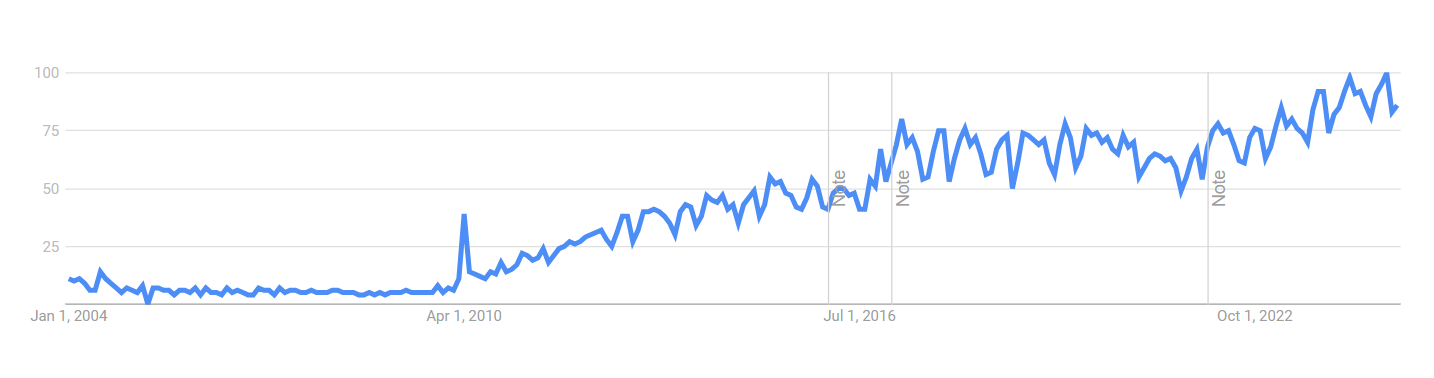
\includegraphics[width=\textwidth]{open_data_google_trends}
    \caption[Open Data su Google Trends]{Ricerche su Google relative al termine Open Data effettuate dal 2004 al 2025. Notare l'aumento successivo al 2009 e il trend in crescita \cite{Google_Trends}.}
    \label{fig:open_data_google_trends}
\end{figure}

\subsection{Concetto di Open Data}
%Definizione e principi fondamentali
Gli \textit{open data}, specialmente quelli della pubblica amministrazione, costituiscono una formidabile risorsa che ancora oggi rimane in larga parte inutilizzata. Molte persone e organizzazioni raccolgono una vasta gamma di svariati tipi di dati per svolgere le proprie attività. In questo ambito, il governo riveste particolare importanza, sia per la quantità e la centralità dei dati che raccoglie, sia perché la maggior parte dei dati del governo sono pubblici per legge, quindi potrebbero diventare aperti e resi disponibili per l'utilizzo da parte di chiunque. Questo riveste particolare interesse in quanto si ritiene che gli \textit{open data} possano apportare benefici in molti settori, ed esistono altrettanti esempi di come siano già stati usati con successo. Ci sono inoltre svariati gruppi di persone e organizzazioni che possono trarre vantaggi dalla disponibilità di \textit{open data}, incluso il governo stesso. Allo stesso tempo, è impossibile effettuare previsioni esatte su come e dove verranno apportati questi benefici in futuro, in quanto è nella stessa natura dell'innovazione che gli sviluppi spesso partano dai posti più inaspettati \cite{OpenDataHandbook_WhyOpenData}.

\subsection{Caratteristiche principali degli Open Data}
% Accessibilità, Interoperabilità, Riutilizzabilità
% Formati comuni: CSV, JSON, XML
In base a quanto stabilito dalla \textit{Open Definition}, gli \textit{open data} sono dati che possono essere utilizzati liberamente e ridistribuiti da chiunque e sono sottoposti, al massimo, al riconoscimento obbligatorio di una potenziale attribuzione o crediti in generale \cite{OpenDefinition}. Nella \textit{full Open Definition} vengono specificate in dettaglio le proprietà più importanti, ovvero:

\begin{itemize}
    \item \textbf{Disponibilità e Accesso:} i dati devono essere disponibili per intero, senza pagare più di un costo ragionevole di riproduzione, preferibilmente scaricandoli dalla rete Internet. I dati devono, inoltre, essere disponibili in un formato conveniente e modificabile.
    \item \textbf{Riutilizzo e Ridistribuzione:} i dati devono essere forniti sotto licenza che ne permetta liberamente il riutilizzo e la ridistribuzione, incluso specialmente il mescolamento con altri \textit{dataset}.
    \item \textbf{Partecipazione Universale:} tutti devono essere in grado di utilizzare, riutilizzare e ridistribuire i dati, senza discriminazioni contro campi di applicazione o contro persone o gruppi particolari. Ad esempio, non sono permesse le licenze ristrette ai soli scopi non-commerciali, che impedirebbero l'utilizzo commerciale, e nemmeno qualsiasi altra restrizione all'uso per certe finalità, come quella esclusivamente educativa.
\end{itemize}

Queste regole sono necessarie per garantire chiarezza sul significato di apertura e, soprattutto, per assicurarne l'\textit{interoperabilità}. Quest'ultima denota la capacità di lavorare insieme, ovvero interoperare, tra diversi sistemi e organizzazioni, che in questo caso si riferisce all'interoperabilità, detta anche mescolanza, tra dataset differenti. \`E una capacità molto importante perché permette a diversi componenti di collegarsi per lavorare insieme e questo è essenziale per realizzare sistemi grandi e complessi, la cui costruzione altrimenti sarebbe quasi impossibile senza interoperabilità \cite{OpenDefinition_Full}.

Il principio cardine di un \textit{commons} di dati o codice, ovvero una raccolta di essi, è che un qualunque pezzo di materiale aperto lì contenuto possa essere mescolato liberamente con altro materiale aperto. Questa interoperabilità è assolutamente necessaria a livello pratico per realizzare i principali benefici ottenibili dall'apertura dei dati, ovvero l'abilità notevolmente migliorata di combinare insieme diversi dataset e di conseguenza la capacità di sviluppare un numero maggiore di prodotti e servizi aventi qualità migliore. Questa definizione data riguardo all'apertura assicura che, dati due dataset aperti ottenuti da due fonti diverse, possiamo essere sempre in grado di combinarli insieme, evitando di trovarci di fronte a un numero enorme di dataset aventi scarsa o nulla capacità di essere mescolati insieme in sistemi di più larga scala, senza quindi avere la capacità di apportare valore aggiunto. Il punto chiave di aprire i dati deve essere il \textit{focus} su dati non-personali, ovvero i dati non devono contenere informazioni riguardanti persone specifiche. Inoltre, per alcuni tipi di dati ottenuti dal governo, potrebbero applicarsi restrizioni nazionali per motivi di sicurezza \cite{OpenDataHandbook_WhyOpenData}.

\subsection{Formati principali}
Gli open data possono essere utilizzati in svariati formati, di seguito vediamo quali.
\subsubsection{JSON}
Quello più utilizzato in ambito software è JSON, un semplice formato file che è molto facile da leggere per qualsiasi linguaggio di programmazione. La sua semplicità lo rende più veloce da processare per un computer rispetto ad altri formati come XML.
\subsubsection{XML}
XML è un formato molto utilizzato per lo scambio di dati, in quanto fornisce buone opportunità di mantenere la struttura dei dati e il modo in cui i file sono costruiti, permettendo agli sviluppatori di scrivere parti della documentazione insieme ai dati senza interferire con la loro lettura.
\subsubsection{RDF}
RDF è un formato raccomandato dal W3C e rende possibile rappresentare i dati in una forma in cui sono più facili da combinare con altri dati provenienti da più fonti. Dati RDF possono essere salvati in varie serializzazioni, tra cui XML e JSON. RDF incoraggia l'utilizzo di URL come identificatori, fornendo un modo conveniente di interconnettere direttamente iniziative open data già esistenti sul Web. Non è ancora molto diffuso, ma è diventato un trend tra le iniziative di Open Government, tra cui annoveriamo i progetti di Open Data collegati tra i governi di Regno Unito e Spagna. L'inventore di Internet, Tim Berners-Lee, ha recentemente proposto uno schema chiamato \textit{fivesstar} che include i dati RDF collegati, ponendolo come obiettivo da raggiungere per le iniziative di open data.
\subsubsection{\textit{Spreadsheet}}
Sono utilizzati da molte autorità, le quali hanno ancora delle informazioni rimaste in documenti come quelli di Microsoft Excel. Questi dati possono essere utilizzati immediatamente con la corretta descrizione del significato delle varie colonne. Tuttavia, in alcuni casi ci possono essere delle macro e delle formule nei fogli di calcolo, che possono diventare potenzialmente più complicate da gestire. Di conseguenza, è consigliabile documentare questo genere di calcoli di fianco allo \textit{spreadsheet}, dato che è generalmente più accessibile alla lettura da parte degli utenti.
\subsubsection{\textit{Comma-Separated Values}}
I file CSV possono essere un formato molto utile data la loro compattezza e possono quindi essere adatti al trasferimento di grandi quantità di dati all'interno della stessa struttura. Tuttavia, questo formato è talmente spartano che i dati sono spesso inutili senza appropriata documentazione, dato che può essere quasi impossibile indovinare il significato delle diverse colonne. Diventa quindi particolarmente importante che la documentazione dei singoli campi sia accurata. Inoltre, è essenziale rispettare la struttura del file, in quanto la singola omissione di un campo è in grado di disturbare la lettura di tutti i rimanenti dati del file senza avere una reale opportunità di aggiustamento, perché non si può determinare come vanno interpretati i dati rimanenti.
\subsubsection{Documento di testo}
I documenti classici in formati come Word, ODF, OOXML o PDF potrebbero bastare per mostrare alcuni tipi di dati, come delle \textit{mailing lists} relativamente stabili o equivalenti, senza richiedere un grande sforzo. Questo formato non offre alcun supporto per il mantenimento di una struttura coerente, il che spesso significa che diventa difficile inserire dati mediante strumenti automatizzati. Bisogna assicurarsi di utilizzare dei \textit{templates} come base dei documenti che mostreranno dati per il riuso, così da rendere possibile ottenere informazioni da tali documenti. Inoltre, per supportare ulteriormente l'utilizzo dei dati si potrebbero utilizzare dei \textit{markers} tipografici il più possibile, così da rendere più facile per una macchina la distinzione degli \textit{headings}, ovvero i titoli di qualsiasi tipo, dal contenuto, e così via. Generalmente è raccomandabile non esibirli in un formato di \textit{word processing}, se i dati esistono in formati differenti.
\subsubsection{Testo non formattato}
I documenti di testo non formattato (.txt) sono molto semplici da leggere per un computer, ma generalmente escludono metadati strutturali dall'interno del documento, quindi gli sviluppatori devono creare un \textit{parser} che possa interpretare ogni documento nell'ordine in cui appare. Possono verificarsi alcuni problemi dallo scambio di file \textit{plain text} tra diversi sistemi operativi, in quanto Windows, macOS e altre varianti Unix hanno ciascuno il loro modo di indicare al computer che si è raggiunta la fine della riga, quindi 3 diversi caratteri di \textit{newline}.
\subsubsection{Immagini scannerizzate}
Probabilmente questo è il metodo meno indicabile per la maggioranza dei dati, ma sia TIFF che JPEG-2000 sono in grado di dargli una documentazione di ciò che si trova nell'immagine, e possono addirittura indicare testualmente l'intero contenuto del documento all'interno di un'immagine dello stesso documento. Potrebbe essere rilevante mostrare dati come immagini i cui dati non sono stati creati elettronicamente, un esempio sono i materiali di archivio, per i quali avere un'immagine è sicuramente meglio di nulla.
\subsubsection{Formati proprietari}
Alcuni sistemi dedicati hanno i propri formati di dati con cui possono essere salvati o esportati. Talvolta può bastare esporre i dati in tale formato, specialmente se ci si aspetta che un ulteriore utilizzo avvenga in un sistema simile a quello da cui provengono. Va sempre indicato dove si possono trovare ulteriori informazioni su questi formati proprietari, per esempio fornendo un link al sito web del fornitore. Generalmente, se fattibile, è raccommandabile mostrare i dati in formati non-proprietari.
\subsubsection{HTML}
Al giorno d'oggi, molti dati sono disponibili in formato HTML su vari siti e questo potrebbe tranquillamente essere sufficiente se i dati sono molto stabili e con ambito limitato. In alcuni casi, però, potrebbe essere preferibile avere i dati in una forma più facile da scaricare e manipolare, ma dato che il riferimento a una pagina su un sito web è una modalità molto semplice ed economica, potrebbe costituire un buon punto di partenza nella visualizzazione di dati. Tipicamente, sarebbe più appropriato utilizzare delle tabelle in documenti HTML per contenere i dati, ed è importante che i vari campi di dati siano visualizzati e assegnati degli ID che li rendano facili da trovare e manipolare i loro dati. Per effettuare lo scraping, Yahoo ha sviluppato un \textit{tool} in grado di estrarre informazioni strutturate da un sito, e tali strumenti sono in grado di effettuare molte altre operazioni purché i dati siano accuratamente etichettati \cite{YahooDevelopers_YQL}.
\subsubsection{Formati Open File}
Anche se le informazioni sono fornite in formati elettronici, dettagliati e comprensibili da un computer (\textit{machine-readable}), potrebbero ugualmente verificarsi problemi relativi al formati del file stesso. I formati in cui le informazioni sono pubblicate, ossia la base digitale in cui le informazioni sono salvate, possono essere sia aperti che chiusi. Un formato aperto è uno in cui le specifiche per il software sono disponibili a tutti e in maniera gratuita, così che chiunque possa utilizzare queste specifiche nel loro software senza limitazioni al riuso imposte dai diritti sulla proprietà intellettuale. D'altro canto, se un formato file è chiuso, potrebbe essere sia perché è proprietario e le specifiche non sono disponibili al pubblico, o perché il formato file è proprietario ma il riuso è limitato, anche se le specifiche sono state rese pubbliche. Se le informazioni sono rilasciate in un formato chiuso, questo può causare ostacoli significativi al riuso delle informazioni in esso racchiuse, costringendo chi sia interessato a utilizzarle a comprare il software necessario. Il beneficio dei formati file aperti è che permettono agli sviluppatori di produrre più pacchetti software e servizi che utilizzano questi formati, minimizzando così gli ostacoli al riuso delle informazioni che contengono. Utilizzare formati file proprietari per i quali le specifiche non sono disponibili pubblicamente può generare una dipendenza su software di terze parti o sui detentori delle licenze del formato file, il che potrebbe significare, nello scenario peggiore, che sia possibile leggere le informazioni esclusivamente utilizzando certi pacchetti software, i quali potrebbero avere un costo proibitivo, o anche diventare obsoleti. Di conseguenza, per i dati aperti forniti dal governo vige la forte preferenza per cui le informazioni dovrebbero essere rilasciate in formati file aperti e \textit{machine-readable}, leggibili da un computer \cite{OpenDataHandbook_FileFormats}.

\subsection{Confronto con dati privati}
Differenze principali

Vantaggi e svantaggi rispetto agli Open Data

\subsection{Contesto italiano e internazionale}
Ad oggi, è già possibile indicare un cospicuo numero di settori nei quali i dati aperti del governo stanno già apportando un certo valore, tra cui:

\begin{itemize}
    \item Controllo di trasparenza e democrazia.
    \item Partecipazione.
    \item Autopotenziamento.
    \item Miglioramento o creazione di nuovi prodotti e servizi da parte di privati.
    \item Innovazione.
    \item Miglioramento dell'efficienza di servizi del governo.
    \item Miglioramento dell'efficacia di servizi governativi.
    \item Misuramento dell'impatto di certe politiche.
    \item Nuova conoscenza ottenuta dalla combinazione di fonti di dati e dalla ricerca di \textit{pattern} all'interno di grandi volumi di dati.
\end{itemize}

Riguardo alla trasparenza, esistono progetti come il finlandese \textit{tax tree}, l'albero delle tasse, e il britannico \textit{where does my money go}, dove vanno i miei soldi, per visualizzare in che modo i ricavi derivanti dalle tasse vengono spesi dal governo. Inoltre, possiamo ricordare come gli open data abbiano risparmiato al Canada \$3.2 miliardi in una frode fiscale relativa a un ente di beneficenza. Altri siti web includono il danese \textit{folketsting.dk} per tracciare l'attività in parlamento e i processi di creazione di leggi, così da poter vedere esattamente gli eventi che stanno accadendo, e quali parlamentari sono coinvolti.
Gli open data del governo possono anche aiutarci a prendere decisioni migliori nella nostra vita, o a diventare più attivi nella società. Una donna in Danimarca ha sviluppato \textit{findtoilet.dk}, che mostra tutti i bagni pubblici danesi così che le persone che conosceva con problemi alla vescica potessero diventare più sicuri di se stessi quando andavano nuovamente fuori. In Olanda è disponibile un servizio, \textit{vervuilingsalarm.nl}, che ci avvisa con un messaggio se domani la qualità dell'aria nelle vicinanze raggiungerà una soglia che abbiamo definito in precedenza. A New York possiamo facilmente capire dove possiamo portare il cane a passeggio, insieme a trovare altre persone che frequentano gli stessi parchi. Servizi come \textit{mapumental} nel Regno Unito e \textit{mapnificent} in Germania permettono di trovare dei posti in cui vivere, prendendo in considerazione la durata del tragitto per arrivare a lavoro, il prezzo delle case e la qualità di una certa zona. Tutti questi servizi, per funzionare, si appoggiano a dati forniti apertamente dal governo.
Economicamente, gli open data sono altrettanto importanti: diversi studi hanno stimato il valore economico degli open data in alcune decine di miliardi di Euro su base annua, e questo solamente nell'Unione Europea. Nuovi prodotti e aziende stanno riutilizzando dati aperti, come ad esempio il danese \textit{husetsweb.dk} che aiuta a trovare dei modi per migliorare l'efficienza energetica della propria casa, insieme alla pianificazione finanziaria e alla ricerca di costruttori che possano svolgere il lavoro. Tutto è basato sul riutilizzo delle informazioni catastali e informazioni sui sussidi da parte del governo, insieme al registro commerciale locale. Google Traduttore utilizza un enorme quantità di documenti dell'UE che compaiono in tutte le lingue europee per addestrare gli algoritmi di traduzione e quindi migliorare la sua qualità del servizio.
Gli open data offrono del valore anche al governo stesso, ad esempio per aumentarne l'efficienza. Il Ministero Olandese dell'Istruzione ha pubblicato online tutti i suoi dati relativi all'istruzione, permettendone il riuso. Da allora, il numero di domande che hanno ricevuto è crollato, riducendo il carico di lavoro e i relativi costi, mentre per i dipendenti pubblici è più facile rispondere alle rimanenti domande, in quanto diventa maggiormente chiaro dove possono essre trovate le informazioni rilevanti. Gli open data hanno anche reso più efficiente la pubblica amministrazione, il che porta a un'ulteriore riduzione dei costi. Il dipartimento olandese dei beni culturali sta rilasciando attivamente i loro dati e collabora con società amatoriali di storia e gruppi come la \textit{Wikimedia Foundation} per eseguire i loro compiti in maniera più efficiente. Questo non solo porta a miglioramenti nella qualità dei loro dati, ma contribuisce anche a rimpicciolire le dimensioni del dipartimento stesso.
Anche se ci sono già numerose istanze relative ai modi in cui gli open data stanno creando del valore aggiunto sia in ambito sociale che in quello economico, non sappiamo ancora nulla riguardo alle nuove cose che diventeranno possibili. Nuove combinazioni di dati possono creare ulteriore conoscenza, il che può potenzialmente portare a scoprire campi di applicazione completamente nuovi. Lo abbiamo già visto in passato, per esempio quando nel XIX secolo a Londra il Dott. Snow ha scoperto il legame tra inquinamento dell'acqua potabile e colera, combinando i dati delle morti attribuibili al colera con la posizione dei pozzi d'acqua. Questo portò alla costruzione dei sistemi fognari di Londra e migliorò notevolmente la salute pubblica della popolazione. Probabilmente potremmo vedere accadere nuovamente degli sviluppi simili, scaturiti dalla combinazione di diversi dataset aperti. Questo potenziale, ancora non sfruttato, può essere rilasciato se trasformiamo i dati pubblici del governo in open data, ma solo se sono davvero aperti, ovvero se non sottoposti ad alcun tipo di restrizione legale, finanziaria o tecnologica relativa al suo riutilizzo da parte di terzi. Ogni restrizione impedisce alle persone di riutilizzare i dati pubblici, o quantomeno lo rende più difficile. Per poter realizzare appieno il loro potenziale, i dati pubblici devono essere aperti, ovvero degli open data \cite{OpenDataHandbook_WhyOpenData}.

\subsubsection{Iniziative globali}
Open Government Partnership

\subsubsection{Normativa italiana}
CAD (Codice dell'Amministrazione Digitale)

\subsubsection{Portali di Open Data}
dati.gov.it

Open Data Bologna (https://opendata.comune.bologna.it/)

\subsubsection{Casi studio e iniziative significative}
INSPIRE

Copernicus


\section{Bologna e progetto BolognaWiFi}  %  e Comune di Bologna
\subsection{Bologna Smart City}
Il progetto di Bologna Smart City è iniziato il 30 luglio 2010, quando il Comune di Bologna, l'Alma Mater e Aster hanno firmato un Protocollo d'intesa per la realizzazione della relativa piattaforma, avente l'obiettivo di rispondere ai bisogni della comunità per migliorarne la qualità della vita e garantire i diritti fondamentali della socialità, dell'istruzione, dello sviluppo e della salute.
Le Smart Cities sono aree urbane intelligenti e sostenibili, in grado di pianificare in modo coerente l'integrazione delle diverse caratteristiche dell'identità del proprio territorio, siano esse economiche, produttive o ambientali, in un'ottica di innovazione.
Bologna ha scelto di intraprendere questo percorso per sviluppare soluzioni utili ad affrontare problematiche urbane e sociali, mettendo la tecnologia al servizio delle persone, attraverso un'alleanza tra mondo della ricerca, Università, imprese e pubblica amministrazione. Basandosi su questa definizione, la città di Bologna vuole essere pensata come un sistema intelligente e sostenibile dove si sfrutta l'ottimizzazione delle risorse per qualificare i servizi già esistenti e crearne di nuovi per costruire una città aperta alla partecipazione e al contributo creativo dei cittadini, ovvero il \textit{civic commons}, così come previsto dal Piano Strategico Metropolitano. Questo accordo sottoscritto ha anche lo scopo di implementare le attività svolte finora da Comune, Alma Mater e Aster sul tema delle Smart Cities ed è aperto all'adesione di altri enti e imprese.
Una città è intelligente se compie delle scelte nette e sostenibili, per cui bisogna investire con azioni strategiche nel campo di energia, servizi, digitale e valorizzazione dei beni ambientali e culturali. In questo ruolo, l'Università mette a disposizione i propri saperi, consapevole del suo legame storico con Bologna, figurandosi come un grande consulente sullo sviluppo della città, della società e dell'impresa. Bologna Smart City è un obiettivo prioritario affinché la regione Emilia-Romagna sia in grado di restare al passo con i tempi, in cui l'innovazione è fondamentale per la competitività imprenditoriale e per il sistema della ricerca, proprio a partire dalla rete di alta tecnologia.
In questo progetto, i tre partner (Comune, Università e Aster) hanno individuato un primo gruppo di 7 ambiti chiave su cui verteranno le azioni sui temi principali:
\begin{itemize}
    \item Beni Culturali: valorizza e riqualifica il centro storico e il suo patrimonio culturale, insieme ai portici e al turismo.
    \item Iperbole 2020 Cloud \& Crowd: riprogetta la Rete Civica Iperbole, basandosi sulla tecnologia cloud e un'identità digitale integrata, raccogliendo così l'offerta di contenuti e servizi di Pubblica Amministrazione, imprese e cittadini.
    \item Reti intelligenti: smart grid, banda ultralarga FTTH e smart lighting.
    \item Mobilità sostenibile: sviluppo di una rete della mobilità elettrica intelligente.
    \item Quartieri sicuri e sostenibili: ristruttura il patrimonio pubblico e privato per aumentare l'efficienza e la produzione di energia, monitora la sicurezza degli edifici, gestisce i rifiuti, configura il social housing, la domotica, il co-working, insieme a servizi e nuovi ambienti per lavoratori della conoscenza e ricercatori.
    \item Sanità e Welfare: e-care, e-health, ottimizzazione dei processi e business intelligence.
    \item Educazione e istruzione tecnica: sviluppo progetti in ambito educativo, promuove una nuova cultura tecnica e scientifica \cite{Bologna_Smart_City}.
\end{itemize}


Bologna è sempre di più una smart city e ha l'obiettivo di diventare una città sostenibile. Si trova già da anni ai primi posti delle classifiche delle smart city italiane. Una città che punta non solo ad essere inclusiva, sicura, attenta alla salute e all'ambiente, ma anche a fornire a tutti i suoi abitanti una serie di servizi tra cui in primis ci sono quelli della mobilità. Sappiamo che l'inquinamento atmosferico è un serio problema per la salute delle persone ed è legato alle emissioni, quindi una città smart sostenibile dovrebbe mettere a disposizione dei cittadini tutta una serie di sistemi volti a ridurre i livelli di CO\textsubscript{2}, particolato e altre sostanze pericolose. Nasce quindi il concetto di MaaS, Mobility as a Service, che consiste in una nuova idea di mobilità in cui si prevde l'integrazione dei vari servizi di trasporto pubblico e privato in un unico canale digitale, rendendoli più accessibili all'utente finale, e questa sharing mobility è già in sperimentazione a Milano. In questo modo, i cittadini possono scegliere tra varie soluzioni di mobilità sostenibile, configurandole come un'alternativa all'utilizzo dell'auto privata. A Bologna ne sono già un esempio il servizio di car-sharing elettrico e di bike-sharing, sia con biciclette classiche che con e-bike (biciclette a pedalata assistita): tutti questi servizi sono noleggiabili tramite una semplice app. Inoltre, a Bologna è attivo il servizio di Telepass Pay, che permette tramite app di pagare il parcheggio, prenotare un taxi, o prenotare la pulizia dell'auto e della moto nel punto in cui è parcheggiata. La tecnologia svolgerà sempre di più un ruolo fondamentale nella diffusione di questi servizi, sempre più diversificati e disponibili, permettendo al cittadino di scegliere il mezzo di trasporto più idoneo al tragitto da compiere e al contempo diminuendo il traffico in città, migliorando la qualità dell'aria e riducendo le emissioni \cite{Bolognatoday_Smart_City}.

\subsubsection{Digitalizzazione e innovazione urbana}
Progetti principali

\subsubsection{Politiche locali per gli Open Data}
Strategie e risultati

\subsubsection{Infrastrutture digitali recenti}
Implementazioni chiave

\subsection{Progetto BolognaWiFi}
Verso la fine degli anni '90, la rete Internet era sempre più diffusa e stava iniziando a diventare un'infrastruttura comunicativa, costituendo così una grande opportunità al servizio dei cittadini. Di conseguenza alcuni comuni italiani, tra cui quello di Bologna, riuscirono a comprenderne in maniera lungimirante le grandi potenzialità che offriva per costruire nuovi spazi di informazione, relazione e connessione civica.
Così nel 1995 il Comune di Bologna, in collaborazione con l'Alma Mater, creò la rete civica Iperbole, la quale venne pensata e sviluppata come una rete globale-locale. Questo progetto potè nascere proprio a Bologna in virtù di una rara situazione di privilegio riguardante l'innovazione amministrativa, molto più avanzata all'epoca rispetto alle altre città italiane.
La rete Iperbole offriva agli utenti la possibilità di avere accesso a Internet, fornendo anche un indirizzo email gratuito, e in questo modo ha saputo contribuire attivamente all'alfabetizzazione digitale dei cittadini bolognesi.
Iperbole è suddivisa in tre sezioni. Nella prima, quella del Comune, vengono riportate le iniziative e le attività svolte dal Comune di Bologna, così da permettere di rimanere aggiornati sulle tematiche correlate a Sindaco, Giunta, Consiglio Comunale, Elezioni, Turismo, Mobilità, Qualità dell'aria, Casa e Comunicati.
Nella seconda, quella dei Servizi Online, è possibile usufruire di tutti i servizi messi a disposizione dal Comune, come il pagamento di multe e bollettini MAV, la prenotazione per l'URP, la richiesta di un assegno familiare, la presentazione della dichiarazione ISEE e la segnalazione di problemi.
Nella sezione Partecipa, invece, il cittadino può impegnarsi e partecipare attivamente ai processi di collaborazione e cura dei beni comuni.
Negli ultimi anni il Comune di Bologna, in collaborazione con Lepida SpA, ha inaugurato la rete Iperbole Wireless, che offre a cittadini e visitatori un servizio di connessione a Internet tramite WiFi, che si configura come un'evoluzione \textit{mobile} della Rete Civica Iperbole. Tale rete wireless è aperta e non richiede autenticazione.
Dal 1995 ad oggi, Iperbole non è più solo una rete telematica di informazione costante e aggiornata per i cittadini, ma sta diventando un vero e proprio punto di riferimento grazie alla facilità di accesso e alle iniziative di partecipazione civica, rappresentando non solo una grande invenzione tecnologica, ma soprattutto un esempio di innovazione sociale grazie al quale si sono garantiti e messi in atto diritti digitali e di cittadinanza \cite{Iperbole_Citta_Connessa}.

Il Comune di Bologna, in collaborazione con Lepida spa, offre a cittadini e visitatori un servizio di connessione a internet in modalità Wi-Fi come evoluzione \textit{mobile} della Rete Civica Iperbole. Per navigare è sufficiente collegarsi alla rete BolognaWiFi, la quale è aperta e non richiede autenticazione. Nelle aree all'aperto è possibile accedere e navigare tutti i giorni 24 ore su 24, mentre nei luoghi all'interno di edifici si può navigare negli orari di apertura delle strutture che offrono il servizio. Ad oggi ci sono più di 300 hotspot attivi in città \cite{BolognaWiFi_Elenco_Hotspot}.


Già nel 2014, dopo un anno intero di operatività della connessione Wi-Fi pubblica a banda ultralarga, piazza Maggiore a Bologna era riuscita a ottenere il titolo di \textit{piazza più connessa d'Europa}, segno dell'importanza di questo progetto per la città felsinea \cite{Smart_City_Piazza_Connessa_Europa}.

BolognaWiFi è un servizio offerto dal Comune di Bologna e fornisce una connettività wireless gratuita a tutti i cittadini. Nato da una collaborazione con alcuni operatori nel settore delle telecomunicazioni, i primi test sono iniziati nel 2005 in Piazza Maggiore, insieme ad alcune ditte private che hanno aderito al progetto \cite{Bologna_WiFi_Bluetooth}.

\subsubsection{Obiettivi principali}
% Scopi e finalità del progetto
Tra gli obiettivi, Iperbole voleva garantire lo scambio di informazioni non soltanto tra le associazioni, ma anche tra individui, istituzioni e, in generale, con chiunque nel mondo avesse a disposizione un computer e un modem, favorendo forme di partecipazione e collaborazione civica.
Iperbole, tutt'oggi, rappresenta il tentativo di riprodurre in uno spazio digitale tutto quello che è lo spazio della città, creando situazioni di incontro e di confronto nella realtà più ampia che è quella di Internet. Queste realtà virtuali, dette anche agorà elettroniche con un riferimento alla piazza principale dell'antica Grecia, intendono rappresentare un punto di riferimento per il cittadino, una specie di mappa con cui orientarsi, informarsi e partecipare alle attività pubbliche della società \cite{Iperbole_Citta_Connessa}.


Lo scopo principale del progetto BolognaWiFi è quello di abbattere il \textit{digital divide}, agevolare la connettività mediante un servizio gratuito e, allo stesso tempo, favorire i cittadini nelle più svariate attività, a prescindere dal fatto che siano residenti, studenti, pendolari o turisti. L'idea originale era che si potesse navigare gratuitamente, sfruttando una miriade di utilità, tutto rimanendo seduti comodamente a uno dei bar del centro o all'ombra delle Due Torri \cite{Bologna_WiFi_Bluetooth}.


\subsubsection{Tipologie di dati raccolti}
Flussi utenti

Accessi WiFi

Affluenza in aree urbane

\subsubsection{Statistiche recenti}
Dati sull'uso del WiFi pubblico a Bologna

\subsubsection{Risorse utili}
Documentazione ufficiale del progetto

Report e analisi pubblicati dal Comune


\section{Visualizzazione dei dati}  % Analisi e
\subsection{Importanza della visualizzazione}
\subsubsection{Analisi dei dati urbani}
Esempi pratici e benefici

\subsubsection{Supporto decisionale}
Impatti sulle amministrazioni pubbliche

\subsection{Caratteristiche di una buona visualizzazione}
Chiarezza e semplicità

Interattività e Accessibilità

\subsection{Strumenti di visualizzazione}
\subsubsection{Panoramica degli strumenti comuni}
Tableau

D3.js

\subsubsection{Vantaggi e svantaggi degli strumenti}
Breve descrizione comparativa

\subsubsection{Applicazioni pratiche: dati sul traffico in Regno Unito}
% Esempi nelle smart cities
Andrew Nicolson è uno sviluppatore software che è stato coinvolto in una campagna di successo contro la costruzione di una nuova strada, la \textit{Westbury Eastern bypass}, nel Regno Unito. Nell'aprile 2010, Andrew era interessato a ottenere accesso e a utilizzare i dati sul traffico della strada che stavano venendo utilizzati per giustificare le proposte e così è riuscito a ottenere alcuni dei dati rilevanti mediante la libertà di richieste di informazioni, ma il governo locale gli ha fornito i dati in un formato proprietario che può essere letto solamente utilizzando software prodotto da un'azienda chiamata Saturn, che è specializzata in modellazione di traffico e sulle relative previsioni. Non esiste una versione del software di sola lettura, quindi il gruppo di Andrew non aveva altra scelta se non acquistare una licenza software, finendo per pagare £500 (€600) utilizzando uno sconto per studenti. Il pacchetto software principale veniva offerto da Saturn a partire da £13\ 000, oltre €15\ 000, un prezzo fuori misura per la maggioranza dei normali cittadini. Anche se nessuna legge nel diritto dell'informazione garantisce un diritto ad avere l'accesso ai dati in formati aperti, le iniziative open data del governo stanno iniziando ad essere accompagnate da documenti di \textit{policies} che stabiliscono che le informazioni ufficiali debbano essere rese disponibili in formati di file che siano aperti. L'amministrazione Obama ha definito il \textit{gold standard}, con la \textit{Open Government Directive} emessa nel dicembre 2009, la quale decreta che, nella misura praticabile e soggetta a restrizioni valide, le agenzie debbano pubblicare informazioni online in un formato aperto che possa essere recuperato, scaricato, indicizzato e ricercato da applicazioni di ricerca web di utilizzo comune. Un formato aperto è inteso come uno che sia indipendente dalla piattaforma, leggibile dalla macchina e reso disponibile al pubblico senza restrizioni che impediscano il riuso di tali informazioni \cite{OpenDataHandbook_FileFormats}.


\section{Sfide e opportunità}   % Benefici e potenziale degli Open Data
\subsection{Sfide tecniche}
\subsubsection{Gestione di dataset eterogenei}
Problemi e soluzioni

\subsubsection{Scalabilità e performance}
Tecnologie per ottimizzare

\subsection{Aspetti etici e legali}
Quando parliamo di database, dobbiamo innanzitutto effettuare una distinzione tra la struttura e il contenuto: utilizzando il termine \textit{dati} ci riferiamo al contenuto del database, mentre gli elementi strutturali fanno riferimento ad attributi come i nomi dei campi e il modello della struttura dati, ovvero l'organizzazione dei campi sopra citati e le loro interrelazioni. In molte giurisdizioni è probabile che gli elementi strutturali di un database siano coperti da copyright, anche se ciò dipende in una certa misura dal livello di creatività che è stato coinvolto nella creazione della struttura. Tuttavia, in questo caso siamo particolarmente interessati ai dati. Quando parliamo di dati dobbiamo prestare attenzione, in quanto tale parola non è particolarmente precisa e può riferirsi sia a un insieme che a un singolo elemento, ma può anche significare una grande raccolta di dati, come tutto il contenuto del database. Per evitare confusione, riserveremo il termine \textit{contenuto} per riferirci ai singoli elementi, mentre la parola \textit{dati} riguarderà l'intera raccolta. Diversamente da materiali multimediali come testi, musica o film, la situazione legale per i dati varia notevolmente tra diversi Paesi. Tuttavia, la maggior parte delle giurisdizioni gli garantisce alcuni diritti in qualità di raccolta dati. La distinzione tra il contenuto del database e l'intera raccolta diviene particolarmente cruciale per i database fattuali, dato che nessuna giurisdizione garantisce il diritto di monopolio sui fatti individuali, ovvero il contenuto, anche se potrebbe garantire loro dei diritti in qualità di raccolta dati. Per fare un esempio, consideriamo un semplice caso di un database che elenca i punti di fusione di varie sostanze. Mentre l'intero database potrebbe essere protetto dalla legge, così da non permettere a nessuno di accedere, riusare o ridistribuire i suoi dati senza averne il permesso, questo non impedirebbe mai a nessuno di affermare il fatto che la sostanza Y si scioglie alla temperatura Z. Le forme di protezione per le raccolte dati ricadono largamente in due casi: diritto d'autore e diritto \textit{sui generis}. Come abbiamo già sottolineato, non abbiamo nessuna regola generale e la situazione varia in base alla giurisdizione. Di conseguenza, bisogna procedere considerando singolarmente ciascun Paese per delineare, se applicabile, quale dei due approcci sia utilizzato in una particolare giurisdizione. Dobbiamo inoltre notare come, in assenza di protezione legale, molti fornitori di database chiusi, ovvero non aperti, possono utilizzare un semplice contratto combinato con disposizioni legali per proibire la violazione dei meccanismi di controllo dell'accesso e ottenere così dei risultati simili a quelli dati da un diritto formale sull'indirizzo IP. Ad esempio, il provider di un database di citazioni può raggiungere qualsiasi insieme di termini e condizioni che voglia implementare, semplicemente richiedendo agli utenti di autenticarsi tramite una password, o fornendo agli utenti un account e una password alla condizione che l'utente accetti i termini e le condizioni del servizio \cite{OpenDataHandbook_LegalRights}.


\subsubsection{Privacy e anonimizzazione dei dati}
Strumenti e tecniche utilizzate

\subsubsection{Licenze e diritti d'uso}
Regolamenti e pratiche comuni

\subsubsection{Casi noti di violazioni}
Esempi significativi e lezioni apprese


\subsection{Opportunità}
\subsubsection{Trasparenza e coinvolgimento}
Benefici per cittadini e istituzioni

\subsubsection{Pianificazione urbana}
Utilizzo dei dati per migliorare i servizi

\subsubsection{Collaborazioni pubblico-privato}
Partnership per sfruttare al meglio gli Open Data

% \subsection{Fonti per approfondire}
% \subsubsection{Linee guida GDPR}
% Applicazioni rilevanti per i dati urbani

% \subsubsection{Studi accademici}
% Temi su etica e Open Data
\clearpage{\pagestyle{empty}\cleardoublepage}
\chapter{Tecnologie Utilizzate}
In questo capitolo presenteremo le varie tecnologie utilizzate per la realizzazione del progetto, descrivendole in modo da fornire una conoscenza di base abbastanza solida da permettere la comprensione dell'ambiente.

\section{HTML}
HTML, acronimo che significa \textit{HyperText Markup Language}, è un linguaggio di markup che permette di impaginare e formattare pagine web collegate tra loro tramite link. Un ipertesto non è altro che l'albero di navigazione che collega le pagine web, ovvero un flusso infinito di pagine collegate tra loro attraverso dei link che permettono di spostarsi da un contenuto all'altro.

HTML risponde all'esigenza di riuscire a pubblicare del testo online, mantenendo la formattazione e il significato di ciascuna delle sue parti, utilizzando dei marcatori detti \Verb_<tag>_. Il browser legge il tag e il suo contenuto, quindi traduce a schermo il codice usando i criteri specificati da HTML. Questo ha permesso di costruire pagine con  una struttura simile fra di loro e soprattutto replicabile seguendo uno standard. Nel giro di pochi anni furono aggiunti via via sempre più tag ed elementi per consentire la creazione di pagine contenenti immagini, elementi interattivi, form, pulsanti, tabelle e altri ancora. Pertanto, HTML si è trasformato in un linguaggio molto completo ma in continuo mutamento, che oggi viene mantenuto dal World Wide Web Consortium (W3C), una associazione non governativa che si occupa di implementare nuove funzioni per rendere il web sempre più libero e accessibile.

Riguardo ai tag, sono alla base dell'HTML e ciascuno di essi corrisponde a un determinato tipo di contenuto. Ogni tag può avere degli attributi specifici, cosa che permette di costruire pagine diverse tra di loro e in modo tale che rispondano alle necessità di chi le scrive. Le pagine in HTML hanno una struttura ad albero: proseguendo lungo la ramificazione, si possono trovare più o meno elementi che costruiscono la pagina stessa seguendo una precisa gerarchia. Ad esempio, nel seguente frammento di codice:
\begin{verbatim}
    <html>
        <head>
            <title>Titolo</title>
        </head>
        <body>
            <p>Paragrafo</p>
        </body>
    </html>
\end{verbatim}
\Verb_<html>_ indica l'inizio della parte di codice che verrà espressa utilizzando il linguaggio HTML. Tranne alcuni tag detti \textit{self-closing tags}, tutti vanno chiusi mediante il rispettivo tag di chiusura, che in questo caso è \Verb_</html>_.
\Verb_<head>_ specifica l'header della pagina, il quale racchiude delle informazioni importanti per il suo funzionamento, ma invisibili dal nostro dispositivo. Contiene a sua volta un \Verb_<title>_, ovvero un titolo che è quello rappresentativo della pagina stessa e del suo contenuto. Una volta chiusa l'intestazione, si passa al \Verb_<body>_, cioè il contenuto della pagina. Al suo interno troviamo il tag \Verb_<p>_, utilizzato per scrivere paragrafi di testo, al cui interno viene scritto il rispettivo contenuto. Tutti i vari browser web sono pensati per interpretare i tag più o meno ugualmente ogni volta, ma ci possono essere eccezioni in quanto ogni browser implementa un proprio rendering della pagina web.

HTMl non è un linguaggio di programmazione, bensì un linguaggio di markup: descrive al browser com'è fatta la struttura di una pagina, e niente più. Un linguaggio di programmazine, invece, ha un ruolo funzionale: risolve cicli di codice seguendo una struttura fatta di \Verb_if_ e \Verb_else_, può svolgere calcoli matematici, può manipolare dati e variabili. Quindi, è il browser web che è programmato per capire la struttura delle pagine scritte in HTML, mentre quest'ultimo descrive soltanto la struttura della pagina e del suo contenuto. Di conseguenza, HTML non è un linguaggio di programmazione, mentre lo sono ad esempio JavaScript e PHP.

Ad oggi non è più sufficiente utilizzare solo HTML per realizzare contenuti web, in quanto le esigenze sono da tempo cambiate: ai siti web serve più di soli contenuti testuali, quindi vengono usati anche altri linguaggi, tra cui CSS e JavaScript, che consentono di scrivere pagine ricche e complete, sia nell'aspetto di grafica che nel comportamento \cite{HTML}.

\section{CSS}
CSS, acronimo di \textit{Cascading Style Sheets}, è un linguaggio di stile per i documenti web. I CSS forniscono istruzioni a un browser o a un altro programma utente su come il documento debba essere presentato all'utente, definendone proprietà come il font, i colori, le immagini di sfondo, il layout, il posizionamento delle colonne o di altri elementi della pagina.

CSS è un linguaggio nato per essere il complemento ideale di HTML, per questo i due linguaggi hanno sempre proceduto parallelamente: nelle intenzioni del W3C, HTML è un semplice linguaggio strutturale, estraneo a qualunque scopo che riguardi la presentazione di un documento. Invece, CSS è lo strumento designato proprio per arricchire l'aspetto visuale e la presentazione di una pagina, nato per separare il contenuto dalla presentazione \cite{CSS_Introduzione}.

Anche CSS è un \textit{living standard} come HTML e per questo viene regolarmente sviluppato dal W3C. Il suo compito principale è definire il design di un sito web e per questo scopo vengono assegnati determinati valori agli elementi HTML con l'aiuto delle proprietà del linguaggio di stile. Queste regole hanno una struttura di base che corrisponde allo schema \Verb_selettore { dichiarazione }_. Un selettore non è altro che una rappresentazione dell'elemento HTML al quale fa riferimento la regola, mentre la dichiarazione consiste dalla combinazione tra proprietà e valore che viene annotata tra due parentesi graffe. Ogni dichiarazione finisce con un punto e virgola, come ad esempio \Verb_h2 { color: #ff0000; }_, nel quale il selettore \Verb_h2_ rappresenta le intestazioni di secondo ordine, ovvero i sottotitoli. La dichiarazione, invece, utilizza la proprietà \Verb_color_ per colorare tali sottotitoli di rosso, in questo caso utilizzando un colore espresso in esadecimale per definire impostazioni di colore precise.

CSS supporta diversi selettori in grado di dare istruzioni di regole:
\begin{itemize}
    \item \Verb_selettore_ corrisponde al nome dell'elemento HTML a cui fa riferimento: lo stile viene applicato su tutti gli elementi HTML dello stesso tipo.
    \item \Verb_.selettore_ si rivolge a tutti gli elementi di una classe specifica e si scrive con un punto davanti al nome della classe HTML corrispondente.
    \item \Verb_#selettore_ si riferisce a un unico elemento con un ID specifico. L'integrazione nel codice sorgente HTML avviene grazie all'attributo id, ovvero \Verb_id="identificatore"_.
    \item \Verb_*_ è il selettore universale e si rivolge a tutti gli elementi HTML di un documento.
\end{itemize}

Il CSS può essere dichiarato in vari modi nell'HTML:
\begin{itemize}
    \item Inline: viene definito direttamente sul tag dell'elemento HTML utilizzando l'attributo \Verb_style_. Ha il vantaggio che non è necessario configurare un foglio di stile apposito e ha la priorità elevata, ma nel momento in cui deve essere applicato un blocco di dichiarazioni questo metodo di stile diventa poco chiaro e ridondante.
    \item Interno: viene definito all'interno del tag \Verb_<style>_ nella \Verb_<head>_ del documento HTML.
    \item Esterno: viene definito in un foglio di stile separato, il quale verrà collegato al documento HTML di base utilizzando l'elemento HTML \Verb_<link>_, sempre nella \Verb_<head>_. Può essere riutilizzato in più pagine HTML, semplicemente importandolo ove necessario.
\end{itemize}

\section{SCSS}
SCSS, acronimo di \textit{Sassy Cascading Style Sheets}, è un'estensione di CSS molto popolare che aggiunge funzionalità potenti che aumentano le capacità standard di CSS.

In qualità di linguaggio di script preprocessing, SCSS permette agli sviluppatori di utilizzare variabili, regole annidate (\textit{nested}), \textit{mixins} e funzioni, che semplificano il processo di scrittura e mantenimento di stylesheets complessi. Essendo un superset di CSS, SCSS è pienamente compatibile con CSS e rende più facile creare codice pulito, organizzato e riutilizzabile, migliorando l'efficienza e la scalabilità dei progetti di web development.


SCSS è una delle due possibili sintassi per il preprocessore SASS, o \textit{Syntactically Awesome Style Sheets}. Come ogni preprocessore, SASS viene compilato in codice CSS nativo che funziona su ogni web browser. La vera potenzialità di questo linguaggio si vede sul lato sviluppatore, in quanto permette di scrivere codice SCSS conciso che verrà compilato in un codice CSS più lungo. Per questo, gli sviluppatori possono riuscire a fare di più scrivendo meno, senza compromettere la compatibilità col web.

La differenza principale tra SCSS e CSS è che SCSS è una sintassi per il preprocessore SASS, mentre CSS è un linguaggio di stile che descrive come un browser debba visualizzare gli elementi HTML. SCSS supporta da molto tempo l'utilizzo di variabili in qualsiasi punto dello stylesheet, mentre CSS offre un supporto nativo per le variabili che è relativamente recente e può essere usato solo per salvare valori e tokens della UI. In SCSS, la sintassi può essere annidata, permettendo di effettuare il nesting sia delle proprietà che di altri selettori, mentre in CSS un singolo selettore può annidare proprietà ma non altri selettori. Inoltre, SCSS supporta i mixins, che sono gruppi di dichiarazioni CSS che possono essere riutilizzate all'interno dello stylesheet, il che può essere utile quando utilizziamo prefissi vendor (come -webkit- per Chrome o -moz- per Firefox), animazioni complesse, o altro codice che potrebbe essere riutilizzato in più posti.

La sintassi SCSS e CSS hanno delle somiglianze in comune, ma quella SCSS permette l'utilizzo di funzionalità più avanzate. SCSS utilizza i punti e virgola e l'indentazione per mantenere la formattazione, mentre il normale CSS potrebbe essere più flessibile senza tuttavia offrire le funzionalità avanzate di SCSS. L'utilizzo di SCSS permette di mantenere una codebase più pulita e più facilmente mantenibile.

Per compilare SCSS in CSS si utilizza un compiler SASS, che funziona con entrambe le sintassi SASS e SCSS \cite{SCSS}. Queste due sintassi sono equivalenti, l'unica differenza è che in SASS si elimina l'utilizzo di punti e virgola e parentesi graffe mediante una sintassi \textit{whitespace-sensitive}, rendendolo però incompatibile con CSS \cite{SASS}.

\section{JavaScript}
JavaScript è un linguaggio di scripting, o di programmazione, che permette di implementare funzionalità complesse all'interno delle pagine web, ad esempio ogni volta che un sito debba essere dinamico e non statico, per creare contenuti aggiornati automaticamente, mappe interattive, controllare elementi multimediali, oppure grafiche animate in 2D o 3D. Costituisce il terzo strato dello stack delle tecnologie web standard.

Lato client, il linguaggio JavaScript consiste delle solite funzionalità di programmazione come il salvataggio di valori in variabili, le operazioni su stringhe, e l'esecuzione di codice in risposta a certi eventi che avvengono su una pagina web, come quello di \Verb_click_. Ma ancora più importante, ci permette di utilizzare le funzionalità costruite su altro codice JavaScript client-side, mediante le \textit{Application Programming Interfaces}, o APIs. Queste sono blocchi di codice già pronto che consentono a uno sviluppatore di implementare progammi che altrimenti sarebbero difficili o impossibili da implementare, rendendo questi compiti più semplici da realizzare. Le API possono essere built-in nel browser o di terze parti. Queste ultime verranno approfondite in una sezione successiva. Le API del browser permettono di esporre dati dall'ambiente del computer, o effettuare compiti complessi. Per esempio:
\begin{itemize}
    \item DOM (\textit{Document Object Model}) API: permettono di manipolare HTML e CSS, creando, rimuovendo e cambiando l'HTML, applicando nuovi stili dinamicamente alla pagina, ecc. Per esempio, vengono utilizzate ogni volta che vediamo aprirsi una finestra popup su una pagina, o quando viene visualizzato del nuovo contenuto.
    \item Geolocation API: permettono di recuperare informazioni geografiche, come la posizione GPS corrente.
    \item Canvas e WebGL API: permettono di creare animazioni 2D e 3D.
    \item Audio e Video API: permettono di riprodurre audio e video direttamente in una pagina web, o filmare un video dalla webcam e visualizzarlo su un altro computer.
\end{itemize}

JavaScript è un linguaggio leggermente interpretato: il browser riceve il codice JS originale e lancia lo script, e nei browser moderni viene utilizzata una tecnica di compilazione detta \textit{just-in-time} per migliorare le performance. In questo caso, il codice JS viene compilato in un formato binario più veloce mentre lo script è in esecuzione, così da lanciarlo il più rapidamente possibile. Tuttavia, JavaScript è comunque considerato un linguaggio interpretato, dato che la compilazione avviene a \textit{run-time}, invece che \textit{ahead-of-time}.

JavaScript può essere utilizzato sia client-side che server-side. Lato client, viene eseguito sul computer dell'utente, ad esempio quando visualizziamo la pagina web, viene scaricato il codice client-side del sito web, quindi è eseguito e visualizzato dal browser. Lato server, invece, viene eseguito dal server, per poi inviare i risultati al browser lato client, dove verranno scaricati e visualizzati. Tra i vari linguaggi server, possiamo utilizzare JavaScript nell'ambiente Node.js.

Inoltre, è utilizzato per creare pagine web dinamiche, dove \textit{dinamico} si riferisce all'abilità, sia in client- che server-side JS, di aggiornare la visualizzazione di una webpage o webapp per mostrare cose diverse in circostanze diverse, generando il nuovo contenuto richiesto. Il lato server genera dinamicamente il nuovo contenuto, prendendo i dati dal database, mentre lato client JavaScript crea dinamicamente nuovo contenuto all'interno del browser, prendendo i dati che gli sono stati inviati dal backend. Generalmente questi due approcci lavorano insieme. Una pagina web statica, invece, non aggiorna il contenuto dinamicamente e mostra sempre la stessa schermata \cite{JavaScript}.

\subsection{AJAX}
AJAX, acronimo di \textit{Asynchronous JavaScript and XML}, è una tecnica di sviluppo web in cui una webapp scarica contenuto dal server mediante una richiesta HTTP asincrona, quindi lo utilizza per aggiornare le parti della pagina rilevanti, senza bisogno di ricaricare nuovamente la pagina. Questo può rendere la pagina più responsive, in quanto si richiedono solo le parti che necessitano di essere aggiornate.

AJAX può essere utilizzato per creare \textit{single-page apps}, dove l'intera webapp consiste in un singolo documento che usa AJAX per aggiornare il contenuto in base alle richieste.

Inizialmente, AJAX venne implementato utilizzando l'interfaccia \\\Verb_XMLHttpRequest_, ma l'API di \Verb_fetch()_ è più adatta alle applicazioni web moderne, in quanto è più potente, flessibile, e in grado di integrarsi meglio con le tecnologie web fondamentali come i \textit{service workers}. I framework web moderni offrono astrazioni per AJAX. Tuttavia, ad oggi questa tecnica è talmente diffusa che il termine specifico \textit{AJAX} viene utilizzato raramente \cite{AJAX}.

\subsection{Framework e librerie}
In JavaScript sono disponibili un gran numero di framework e librerie, sviluppati nel corso degli anni per velocizzare e semplificare lo sviluppo web.

Le librerie sono dei pacchetti di classi e funzioni riutilizzabili per risolvere particolari problemi, sono flessibili e possono essere utilizzate liberamente. Alcuni esempi di librerie famose sono:
\begin{itemize}
    \item React.js, utilizzato per creare UI complesse e gestire lo stato.
    \item jQuery, utilizzato per gestire eventi JS ed effettuare chiamate AJAX.
    \item D3.js (\textit{Data-Driven Documents}), utilizzato per la visualizzazione dati.
    \item Chart.js, utilizzato per disegnare vari tipi di grafici utilizzando l'elemento HTML5 \Verb_<canvas>_.
\end{itemize}

I framework, invece, offrono un approccio strutturato allo sviluppo di un progetto, mediante un insieme di strumenti utili a creare applicazioni in maniera standardizzata. Specificano dove inserire quali frammenti di codice e spesso includono funzionalità come la gestione del routing, richieste HTTP, o dei dati di backend. Questo approccio strutturato semplifica lo sviluppo e assicura consistenza tra i vari progetti. Alcuni esempi di framework famosi sono:
\begin{itemize}
    \item Angular, sviluppato da Google, utilizzato per lo sviluppo cross-platform.
    \item Vue.js, utilizzato per creare UI e SPAs (\textit{Single-Page Applications}).
    \item Next.js, framework basato su React per sviluppare webapp multipiattaforma \cite{JS_Frameworks_Libraries}.
\end{itemize}

\`E possibile anche eseguire codice JavaScript al di fuori dal browser, utilizzando l'ambiente di esecuzione Node.js, che è open-source e multipiattaforma \cite{Node.js}.

\section{Leaflet}
Leaflet è una libreria JavaScript open-source che permette di visualizzare mappe interattive mobile-friendly. Il suo codice pesa solo 42KB, ma contiene tutte le funzionalià di mapping che possono servire a quasi tutti gli sviluppatori.

Questa libreria è stata progettata avendo in mente la semplicità, le prestazioni e l'usabilità. Funziona in modo efficiente su tutte le principali piattaforme desktop e mobile, permette l'estensione delle sue funzionalità mediante l'utilizzo di plugins e offre diverse API.

Leaflet non cerca di fare tutto, ma si focalizza sulle funzionalità di base per fare in modo che funzionino perfettamente. Le sue caratteristiche principali sono:
\begin{itemize}
    \item Layers\\
    Offre i cosiddetti \textit{tile layers}, i \textit{markers}, e i popup. Inoltre, si possono mettere delle immagini come overlays e i GeoJSON. Sulla mappa si possono disegnare poligoni, polylines e cerchi.
    \item Interazione\\
    Supporta lo scorrimento, lo zoom tramite gesture, doppio click o scroll wheel, lo spostamento dei marker, gli eventi, e altro ancora.
    \item Funzionalità\\
    Visivamente, supporta le animazioni per lo zoom e il fade. I popup possono essere customizzati tramite CSS, e si può creare un marker personalizzato tramite immagini o HTML. Riguardo alle mappe, gli sviluppatori possono utilizzare i layer che preferiscono.
    \item Controlli\\
    Sono presenti bottoni per lo zoom e il cambio di layer, un'indicatore per la scala, e uno per l'attribuzione \cite{Leaflet_Overview}.
\end{itemize}

\section{Vue.js}
Vue è un framework JavaScript utilizzato per la costruzione di interfacce utente (UI). Si basa sullo standard stack HTML, CSS e JavaScript e offre un modello di programmazione dichiarativo e basato sui componenti, che aiuta a sviluppare in modo efficiente delle UI anche complesse. Le funzionalità chiave di Vue sono due:
\begin{itemize}
    \item Rendering dichiarativo: Vue estende lo standard HTML mediante una sintassi di template che permettono di descrivere output HTML in modo dichiarativo, basato su uno stato definito in JavaScript.
    \item Reattività: Vue traccia automaticamente i cambiamenti di stato in JavaScript e aggiorna il DOM in modo efficiente quando avvengono queste variazioni.
\end{itemize}

Vue è un framework ed ecosistema che copre la maggioranza delle più comuni funzionalità richieste nello sviluppo frontend. Tuttavia, il web è estremamente vario e ciò che viene costruito può cambiare drasticamente in forma e scala. Vue è stato disegnato proprio per rispondere a queste esigenze, in modo da essere flessibile e adottabile in modo incrementale. In base al caso d'uso, Vue può essere utilizzato in diverse modalità:
\begin{itemize}
    \item Miglioramento di HTML statico senza necessità di compilazione.
    \item Integrazione di componenti web su qualsiasi pagina.
    \item Creazione di \textit{Single-Page Applications} (SPA).
    \item Utilizzo di Fullstack o \textit{Server-Side Rendering} (SSR).
    \item Utilizzo di Jamstack o \textit{Static Site Generation} (SSG).
    \item Targeting specifico di desktop, mobile, WebGL, o anche il terminale.
\end{itemize}
Vue è flessibile, ma le sue nozioni principali sono condivise a tutti i livelli, rendendolo un framework adattabile alle esigenze di chiunque \cite{Vue}.

\section{NPM}
NPM, o \textit{Node Package Manager}, è il package manager di default per Node.js. Nel settembre 2022, il registro di NPM conteneva oltre 2.1 milioni di pacchetti, rendendolo il più grande repository al mondo di codice che utilizza un solo linguaggio, possiamo quindi essere quasi sicuri che esista un pacchetto per ogni evenienza. NPM nacque come un modo per scaricare e gestire le dipendenze di Node.js, ma è in seguito diventato uno strumento utilizzato anche nel JavaScript a frontend.

NPM installa, aggiorna e gestisce i download delle dipendenze del progetto. Le dipendenze sono blocchi di codice precostruiti, come le librerie e i pacchetti, di cui l'applicazione ha bisogno per poter funzionare.

Oltre ai normali download, NPM gestisce anche il versioning, così da poter specificare qualsiasi versione specifica di un pacchetto, o richiedere una versione più recente o più vecchia di quella che ci serve. Spesso capita che una libreria sia compatibile solamente con una major release di un'altra libreria, o che un bug nell'ultima versione di una libreria sia ancora irrisolto e continui a causare problemi. Specificare esplicitamente una versione di una libreria aiuta anche a tenere tutto il team sulla stessa versione di un package, così che tutti la utilizzino fino a quando il file \Verb_package.json_ sia aggiornato. In tutti questi casi, il controllo delle versioni aiuta notevolmente e NPM segue lo stesso standard di \textit{semantic versioning}, o \textit{semver}.

NPM consente anche agli sviluppatori di eseguire comandi personalizzati, supportando un formato per specificare task a terminale che vengono lanciati come scripts. Per esempio, utilizzando \Verb_npm run dev_ possiamo lanciare l'app in modalità debug senza scrivere l'effettivo comando corrispondente, che sarebbe molto più lungo. Altri comandi, tra tutti, sono \Verb_npm run prod_ e \Verb_npm run build_ \cite{NPM_Package_Manager}.

\section{PHP}
PHP, acronimo ricorsivo per \textit{PHP: Hypertext Preprocessor}, è un linguaggio di scripting open-source e general-purpose molto usato, che è specialmente adatto per lo sviluppo web e ad essere integrato nell'HTML.

Invece di utilizzare molti comandi per visualizzare l'HTML, come avviene in C o Perl, le pagine PHP contengono HTML all'interno di codice integrato che svolge qualche preciso compito. Il codice PHP è racchiuso in speciali istruzioni di inizio e fine, ovvero \Verb_<?php_ e \Verb_?>_ che permettono di entrare e uscire dalla \textit{modalità PHP}.

Ciò che distingue PHP dal codice JavaScript client-side è che il codice è eseguito sul server, generando HTML che viene quindi inviato al client. Il client riceve così il risultato dell'esecuzione di quello script, senza sapere quale sia il codice sottostante. Un web server può essere configurato per processare tutti i file HTML utilizzando PHP, senza che gli utenti abbiano alcun modo per capire che si stia utilizzando PHP.

PHP riguarda principalmente lo scripting lato server, quindi può fare qualsiasi cosa che altri programmi CGI (\textit{Common Gateway Interface}) sanno fare, come raccogliere dati da un \textit{form}, generare dinamicamente il contenuto della pagina, o inviare e ricevere cookies. Due sono le aree principali dove gli script PHP vengono utilizzati:
\begin{itemize}
    \item Scripting lato server\\
    Questo è il più utilizzato e costituisce il principale campo di applicazione per PHP. Per funzionare, richiede un parser PHP (CGI o modulo server), un server web, e un browser web. Tutti questi possono essere eseguiti localmente per scopi di sviluppo.
    \item Scripting a command line\\
    Uno script PHP può essere eseguito senza richiedere alcun server o browser, basta solo disporre di un parser PHP per poterlo utilizzare in questa maniera. Questo tipo di utilizzo è ideale per script eseguiti regolarmente tramite \Verb_cron_, su Unix e macOS, o con \textit{Task Scheduler} su Windows. Questi script possono essere semplicemente usati anche per processare del testo.
\end{itemize}

PHP può essere utilizzato su tutti i principali sistemi operativi, tra cui Linux, molte varianti Unix come Solaris e OpenBSD, Microsoft Windows, macOS, RISC OS, e altri ancora. PHP supporta anche la maggior parte degli attuali web server, inclusi Apache, IIS, e molti altri, incluso qualsiasi web server in grado di utilizzare \textit{binaries} di FastCGI, come lighttpd e nginx. PHP è in grado di lavorare come modulo o come processore CGI.

Con PHP, gli sviluppatori hanno la libertà di scelta sia per il sistema operativo che per il web server. Inoltre, viene data la possibilità di scegliere se utilizzare un paradigma di programmazione procedurale o uno ad oggetti (OOP), o addirittura di mescolarli.

PHP non si limita a sfornare HTML, ma è in grado di generare file RTF (\textit{Rich File Types}), come immagini o file PDF, criptare dati, e inviare emails. Inoltre, può produrre facilmente qualsiasi tipologia di testo, come JSON o XML. PHP è in grado di generare questi file automaticamente e di salvarli a file system, invece di mostrarli a schermo, formando così una cache a lato server per il contenuto dinamico.

Una delle funzionalità più importanti di PHP è il suo supporto a una grande varietà di database. Scrivere una pagina web che acceda a un db diventa così incredibilmente semplice, utilizzando una delle estensioni specifiche come mysqli per MySQL, o mediante un livello di astrazione come PDO (\textit{Protected Destination of Origin}), oppore connettendosi a un database che supporta lo standard Open Database Connection tramite l'estensioen ODBC. Altri database, invece, possono utilizzare cURL o sockets.

PHP supporta molti protocolli per la comunicazione con altri servizi, ad esempio IMAP, POP3 e HTTP, oltre a molti altri, ed è in grado di aprire dei socket grezzi di rete e interagirvi con qualsiasi altro protocollo. PHP supporta lo scambio di dati complessi tra virtualmente tutti i linguaggi di programmazione utilizzati sul Web. Riguardo all'interconnessione, PHP offre supporto per instanziare oggetti Java e utilizzarli in modo trasparente come oggetti PHP \cite{PHP}.

\section{API}
Le APIs sono meccanismi che permettono a due componenti software di comunicare tra loro utilizzando un insieme di definizioni e protocolli. Ad esempio, vengono utilizzate dalle app meteo nello smartphone, le quali scaricano i dati meteorologici giornalieri effettuando una richiesta alle API meteo corrispondenti per poter visualizzare gli aggiornamenti.

API significa \textit{Application Programming Interface}. Nel contesto delle APIs, Applicazione si riferisce a ogni software con una funzione distinta, mentre Interfaccia è un contratto di servizio tra due applicazioni, che definisce come queste due possano comunicare tra loro utilizzando richieste e risposte. La loro documentazione API contiene informazioni su come gli sviluppatori debbbamo strutturare tali richieste e risposte.

L'architettura API è generalmente spiegata in termini di client e server. L'applicazione che invia la richiesta è detta client, mentre quella che manda la risposta è il server. Quindi, nell'esempio di prima, il server è il database meteo del provider, mentre l'app mobile costituisce il client.

\subsection{Tipologie di API}
Esistono quattro diversi modi in cui le APIs possono funzionare, in base a quando e perché sono state create.
\begin{itemize}
    \item SOAP APIs\\
    Queste API utilizzano un protocollo chiamato \textit{Simple Object Access Protocol}, dove client e server si scambiano messaggi tramite XML. Questa tipologia di API è meno flessibile, ma è stata più popolare in passato.
    \item RPC APIs\\
    Queste API sono chiamate \textit{Remote Procedure Calls}: il client completa una funzione (o procedura) sul server, quindi il server invia il corrispondente output al client.
    \item Websocket APIs\\
    Sono un'altra tipologia di API utilizzate nel moderno sviluppo web e utilizzano oggetti JSON per il passaggio dei dati. Un'API di tipo WebSocket supporta la comunicazione a due vie tra le app client e il server. Il server, a sua volta, può inviare messaggi di callback ai client connessi, rendendolo così più efficiente delle API di tipo REST.
    \item REST APIs\\
    Sono le API più popolari e flessibili che possiamo trovare, ad oggi, sul web. Il client invia richieste al server sotto forma di dati, quindi il server utilizza questo input fornito dal client per eseguire funzioni interne e ritorna i dati di output, inviandoli indietro al client.
\end{itemize}

Oltre all'architettura, le API sono classificate anche in base al loro scopo di utilizzo:
\begin{itemize}
    \item API Private\\
    Sono interne a un'azienda e vengono utilizzate solamente per connettere sistemi e dati all'interno di essa.
    \item API Pubbliche\\
    Sono aperte al pubblico e possono essere utilizzate da chiunque. Tuttavia, potrebbe esserci qualche tipo di autorizzazione e costo associato al loro utilizzo, anche se non necessariamente.
    \item API Partner\\
    Sono accessibili solo agli sviluppatori esterni autorizzati, per incoraggiare le partnership tra business (B2B).
    \item API Composite\\
    Combinano due o più APIs per risolvere requisiti di sistema o comportamenti complessi.
\end{itemize}

\subsection{RESTful APIs}
REST significa \textit{Representational State Transfer} e definisce un insieme di funzioni come GET, PUT, DELETE, e altre, che i client possono utilizzare per accedere ai dati del server. Sia client che server si scambiano dati mediante HTTP.

La funzionalità principale delle API di rest è la mancanza di stato (\textit{statelessness}), ovvero i server non salvano i dati del client tra le varie richieste. Le richieste che il client effettua al server sono simili agli URL utilizzati per visitare un sito web in un normale browser. La risposta fornita dal server consiste in \textit{plain data}, senza alcun tipo di rendering grafico, a differenza di una pagina web.

Una Web API, detta anche Web Service API, è una \textit{application programming interface} tra un web server e un browser. Tutti i web services sono API, ma non tutte le API sono servizi web. Le API REST sono un tipo speciale di Web API che utilizza lo stile architetturale standard che abbiamo visto poco fa.

I diversi termini riguardanti le APIs, come Java API o service API, esistono perché storicamente le API furono create prima del World-Wide Web. Le API web moderne sono REST APIs e i termini possono ormai essere utilizzati in modo intercambiabile.

\subsection{Utilizzo delle API}
Le integrazioni delle API sono componenti software che aggiornano automaticamente i dati tra client e server. Alcuni esempi di integrazioni API sono quando la galleria del telefono viene sincronizzata automaticamente sul cloud, o la data e l'ora del portatile si sincronizzano automaticamente, aggiornandosi quando viaggiamo in un altro fuso orario. Possono inoltre essere utilizzate dalle aziende per automatizzare molte funzioni di sistema in maniera efficiente.

Le REST APIs offrono quattro principali benefici:
\begin{enumerate}
    \item Integrazione\\
    Le API sono utilizzate per integrare nuove applicazioni con sistemi software esistenti. Questo accelera la velocità di sviluppo, in quanto ciascuna funzionalità non ha bisogno di essere riscritta da zero, ma possiamo utilizzare le API per sfruttare codice già esistente.
    \item Innovazione\\
    L'arrivo di una nuova app è in grado di cambiare intere industrie, quindi le aziende devono essere in grado di rispondere velocemente e supportare il rilascio rapido di servizi innovativi. Questo può avvenire apportando cambiamenti a livello delle API, senza dover riscrivere l'intero codice.
    \item Espansione\\
    Le API presentano un'opportunità unica per le aziende di soddisfare le esigenze dei clienti su diverse piattaforme. Per esempio, le Maps API permettono l'integrazione di informazioni relative alle mappe su siti web, Android, iOS, e altri. Qualunque azienda può offrire un simile accesso ai propri database interni, utilizzando API gratuite o a pagamento.
    \item Facilità di manutenzione\\
    Una API funge da porta di passaggio tra due sistemi. Ciascun sistema è obbligato ad apportare cambiamenti interni così da non influenzare il funzionamento delle API. In questo modo, ogni cambiamento futuro al codice effettuato da una qualunque delle due parti non impatterà l'altra.
\end{enumerate}

Gli API endpoints sono il punto finale del sistema di comunicazione delle API e includono URL di server, servizi, e altre locazioni specifiche digitali da cui vengono inviate e ricevute le informazioni tra i diversi sistemi. Gli API endpoints sono di importanza critica per le aziende per due ragioni principli:
\begin{enumerate}
    \item Sicurezza\\
    Gli API endpoints rendono il sistema vulnerabile agli attacchi, quindi il monitoraggio delle API è cruciale per prevenire un utilizzo improprio.
    \item Prestazioni\\
    Gli API endpoints, specialmente quelli ad alto traffico, possono causare bottlenecks (colli di bottiglia) e influenzare le performance del sistema.
\end{enumerate}

Tutte le API quindi devono essere rese sicure tramite appropriata autenticazione e monitoraggio. I due modi principali per mettere in sicurezza le REST APIs includono:
\begin{enumerate}
    \item Token di autenticazione: sono utilizzati per autorizzare gli utenti a effettuare le chiamate alle API, controllano che gli utenti siano correttamente identificati e che abbiano effettivi diritti di accesso per quella particolare chiamata API. Per esempio, quando effettuiamo l'accesso al server email, il client email utilizza token di autenticazione per un accesso sicuro.
    \item Chiavi API: verificano il programma o l'applicazione che effettua la chiamata alle API. Identificano l'applicazione e assicurano che abbia i diritti di accesso richiesti per effettuare quella particolare chiamata API. Le chiavi API non sono sicure come i tokens, ma permettono di monitorare le API per raccogliere dati sul loro utilizzo. Ad esempio, quando visitiamo un sito web e notiamo una lunga stringa di caratteri e numeri nel suo URL, questa stringa è una chiave API che il sito utilizza per effettuare chiamate alle API interne.
\end{enumerate}

\subsection{Documentazione}
Scrivere una documentazione delle API comprensiva è parte del processo di gestione delle API. Tale documentazione può essere generata automaticamente tramite appositi strumenti o scritta manualmente. Come \textit{best practice}, è buona norma scrivere le spiegazioni in linguaggio semplice e facile da leggere, preferibilmente in inglese. I documenti generati con tools possono diventare verbosi e quindi richiedere modifiche manuali. Inoltre, bisogna utilizzare esempi di codice per spiegare le funzionalità e mantenere la documentazione accurata e aggiornata. Lo stile di scrittura va rivolto ai principianti e bisogna coprire tutte le tipologie di problemi che le API possono risolvere per gli utenti \cite{API_AWS}.

\subsection{Evoluzione delle API}
I framework e le librerie possono cambiare le loro APIs. Migrare un'applicazione alle nuove API è tedioso e distrugge il processo di sviluppo: anche se sono stati proposti alcuni strumenti e idee per risolvere l'evoluzione delle API, la maggioranza degli aggiornamenti viene ancora fatta manualmente. Generalmente, i cambiamenti che causano la rottura delle applicazioni esistenti non sono casuali, ma ricadono in particolari categorie: oltre l'80\% di questi è dovuto a \textit{refactorings}, il che suggerisce che per l'aggiornamento delle applicazioni dovrebbero essere utilizzati dei tool di migrazione basati sul refactoring \cite{API_Evolution}.

\section{JSON}
\textit{JavaScript Object Notation}, o JSON, è un formato standard text-based per rappresentare dati strutturati basati su sintassi JavaScript ad oggetti. Viene comunemente utilizzato per trasmettere dati in applicazioni web, ad esempio per inviare dati dal server al client, così da poterlo visualizzare su una pagina web, o viceversa.

Anche se JSON ricorda molto la sintassi JavaScript per creare gli oggetti letterali, può essere utilizzato indipendentemente da JS e molti ambienti di programmazione offrono la capacità di leggere (parse) e generare JSON.

JSON esiste sotto forma di stringa, utile quando vogliamo trasmettere dati sulla rete. Quando vogliamo accedere ai dati, bisogna convertirlo in un oggetto JavaScript nativo, ma questo non è un problema in quanto JS offre un oggetto JSON globale che dispone di metodi per la conversione tra i due. Convertire una stringa in un oggetto nativo è detto \textit{deserializzazione}, mentre il processo inverso in cui si converte un oggetto nativo in una stringa è detto \textit{serializzazione}. Una stringa JSON può essere salvata in un suo proprio file, che consiste praticamente in un file di testo avente l'estensione \Verb_.json_ e un tipo MIME di \Verb_application/json_.

All'interno di un oggetto JSON, possiamo includere gli stessi tipi di dati basilari che utilizzeremo in un oggetto JavaScript standard, ovvero stringhe, numeri, array, booleani e altri ancora. Questo ci permette di costruire una gerarchia di dati che può essere anche annidata e permette l'accesso nello stesso modo in cui si accede ai campi di un analogo oggetto \cite{JSON}.

\section{SQL}
\textit{Structured Query Language} (SQL) è un linguaggio di programmazione utilizzato per salvare e processare informazioni all'interno di un database relazionale, ovvero in forma tabellare, con righe e colonne che rappresentano diversi attributi e le varie relazioni tra i valori. Possiamo utilizzare le istruzioni SQL per salvare, aggiornare, rimuovere, cercare e raccogliere informazioni dal database, inoltre SQL permette di mantenere e ottimizzare le prestazioni del database \cite{SQL}.

\subsection{MySQL}
MySQL è un \textit{Relational Database Management System} (RDBMS) open-source molto popolare, utilizzato per salvare e gestire dati in maniera affidabile, prestante, scalabile e facile da usare. Da qui in poi ci riferiremo a MySQL come versione del database SQL.

\subsection{Struttura dei dati relazionali}
MySQL è un database relazionale open source che utilizza SQL per creare e gestire i database, salvando i dati in tabelle di righe e colonne organizzate in schemi. Uno schema definisce come i dati sono organizzati e salvati, descrivendo le relazioni esistenti tra le varie tabelle. Con questo formato, possiamo facilmente salvare, raccogliere e analizzare diversi tipi di dati, inclusi semplice testo, numeri, date, orari e, recentemente, JSON e arrays.

Due capacità principali di MySQL sono il suo supporto alle transazioni ACID e la sua abilità di essere scalabile. ACID significa \textit{Atomicity, Consistency, Isolation, and Durability}, ovvero le quattro proprietà che assicurano che le transazioni nel database siano processate in modo affidabile e accurato. Mediante le transazioni ACID, MySQL garantisce che tutte le modifiche ai dati siano effettuate in maniera coerente e affidabile, anche nel caso in cui avvenga un guasto nel sistema. MySQL è in grado di scalare per supportare database di dimensioni molto grandi, gestendo un alto volume di connessioni concorrenti. Le prestazioni, la facilità d'uso e il costo contenuto, insieme alla sua capacità di scalare affidabilmente, hanno reso MySQL il database open source più popolare al mondo.

MySQL è veloce, affidabile, scalabile e facile da utilizzare. Originariamente venne sviluppato per gestire rapidamente grandi database ed è stato utilizzato da molti anni in ambienti di produzione con requisiti molto elevati. MySQL offre un ampio insieme di funzioni di utilità ed è sviluppato costantemente da Oracle, così da restare al passo con le nuove richieste tecnologiche e aziendali. La connettività, velocità, e sicurezza di MySQL lo rendono altamente qualificato per l'accesso ai database su Internet. Alcuni dei principali benefici di MySQL includono:
\begin{itemize}
    \item Facilità d'uso: gli sviluppatori possono installare MySQL nel tempo di qualche minuto e il database è facile da gestire.
    \item Affidabilità: MySQL è uno dei database più maturi e ampiamente utilizzati, ed è stato testato in una grande varietà di scenari per quasi 30 anni, incluse molte delle aziende più grosse al mondo, le quali dipendono da MySQL per eseguire applicazioni critiche, data la sua affidabilità.
    \item Scalabilità: MySQL è in grado di scalare per soddisfare i bisogni delle applicazioni con il maggior numero di accessi. La sua architettura a replicazione nativa permette alle aziende, tra cui Facebook, Netflix e Uber, di scalare le applicazioni per supportare decine di milioni di utenti, se non di più.
    \item Prestazioni: MySQL è un sistema di database ad alte prestazioni e con zero necessità di amministrazione, viene rilasciato in diverse edizioni per soddisfare quasi tutte le richieste.
    \item Elevata disponibilità: MySQL offre un insieme completo di tecnologie di replicazione native e pienamente integrate per permettere una grande disponibilità e al contempo il recupero dei disastri. Per le applicazioni di business critiche e gli accordi di servizio, i clienti possono raggiungere l'obiettivo di zero perdite di dati, con un tempo di recupero istantaneo.
    \item Sicurezza: la sicurezza dei dati riguarda sia la protezione degli stessi dati, che il rispetto delle leggi dell'industria e del governo, ingluso il GDPR nell'Unione Europea. MySQL Enterprise è in grado di offrire funzionalità di sicurezza avanzate, come l'autenticazione/autorizzazione, la crittografia trasparente dei dati, l'auditing, il data masking e un firewall per il database.
    \item Flessibilità: il Document Store di MySQL offre agli utenti una massima flessibilità nel sviluppare tradizionali applicazioni database che utilizzino sia SQL che NoSQL, queste ultime senza schemi. Gli sviluppatori possono mischiare tabelle relazionali con documenti JSON nello stesso database e nella stessa applicazione.
\end{itemize}

\subsection{Utilizzo nelle applicazioni web}
I casi d'uso di MySQL includono la gestione di dati dei clienti e dei prodotti per i siti di e-commerce, aiutando i sistemi di gestione dei contenuti a servire contenuti web, tracciare le transazioni in modo sicuro e i dati finanziari, alimentando i siti di social network salvando i profili degli utenti e le loro interazioni.

L'abilità di MySQL di gestire grandi dataset e query complesse lo rende una tecnologia chiave nelle industrie e i casi d'uso includono:
\begin{itemize}
    \item E-commerce: molte delle piattaforme di ecommerce più grandi al mondo, come Uber e Booking.com, eseguono i loro sistemi transazionali su MySQL. Costituisce quindi una scelta popolare per gestire i profili utente, le credenziali, il contenuto degli utenti e i dati finanziari, inclusi pagamenti e rilevamento di truffe.
    \item Piattaforme social: Facebook, X (ovvero l'ex-Twitter) e LinkedIn sono tra le piattaforme social più grandi al mondo e tutti si appoggiano a MySQL per la parte di database.
    \item Gestione del Contenuto: a differenza dei documenti di database \textit{single-purpose}, MySQL offre l'abilità di utilizzare sia SQL che NoSQL all'interno dello stesso database. Il MySQL Document Store permette operazioni CRUD e utilizza il potere di SQL per effettuare data queries sui documenti JSON per riportarne contenuto e statistiche.
    \item SaaS: MySQL è il database sottostante a molte applicazioni popolari di \textit{Software-as-a-Service}, come ad esempio Zendesk \cite{MySQL}.
\end{itemize}

\subsection{Normalizzazione dei dati}
La normalizzazione è il processo di organizzazione dei dati all'interno di un database. Include la creazione di tabelle e lo stabilimento di relazioni tra queste in base a regole definite sia per proteggere i dati, sia per rendere il database più flessibile, eliminando la ridondanza e le dipendenze non coerenti.

I dati ridondanti sprecano spazio su disco e danno luogo a problemi di mantenimento. Se abbiamo bisogno di cambiare dei dati che esistono in più di un posto, tutti i dati vanno modificati nella stessa identica maniera in tutte queste locazioni. Una modifica è invece più facile da implementare se i relativi dati esistono solo in un punto e da nessun'altra parte nel database. Una dipendenza incoerente rende i dati difficili da accedere, in quanto il percorso per trovare tali dati potrebbe essere mancante o malfunzionante.

Esistono alcune regole per la normalizzazione di un database e ciascuna di essere è chiamata una \textit{forma normale}. Generalmente si applicano le prime tre regole per ottenere un database in terza forma normale.

Non sempre però si riesce a rispettare tali regole alla lettera: in generale, la normalizzazione richiede la creazione di tabelle aggiuntive e questo talvolta può risultare scomodo. In questo modo, tuttavia, si generano possibili problemi quali dati ridondanti e dipendenze funzionali \cite{Database_Normalization}.

\section{Apache HTTP Server}
Apache HTTP Server, detto anche semplicemente Apache, è un web server gratuito e open-source che distribuisce contenuti web attraverso la rete Internet, ed è rapidamente diventato il più popolare client HTTP sul web. Il nome trova le sue origini nel rispetto delle tribù dei nativi americani, per la loro resilienza e durabilità.

Apache è solo uno dei componenti richiesti nello stack di un'applicazione web per la distribuzione del contenuto. Uno degli stack più comuni per le webapp è LAMP, ovvero Linux, Apache, MySQL e PHP, o il suo analogo WAMP che utilizza Windows invece che Linux. Il sistema operativo, Linux o Windows, gestisce le operazioni dell'applicazione. Apache è il web server che processa le richieste e serve risorse e contenuti web tramite protocollo HTTP. MySQL è il database che contiene tutte le informazioni in un formato che permette di eseguire queries facilmente. PHP è il linguaggio di programmazione che funziona con Apache per aiutare a creare contenuto web dinamico.

Anche se le statistiche effettive possono variare, gran parte delle webapp vengono eseguite su una qualche forma di stack LAMP in quanto è facile da costruire e utilizzabile in modo gratuito. Generalmente, la maggior parte delle webapp tende ad avere un'architettura simile, anche se il loro scopo può variare considerevolmente, e possono beneficiare dell'utilizzo di Firewalls, Load Balancers, Web Servers, Content Delivery Networks (CDN) e Database Servers.

I Firewall aiutano a proteggere l'applicazione web sia da minacce esterne che da vulnerabilità interne, in base a come sono configurati. I Load Balancers aiutano a distribuire il traffico tra i server web che possono gestire le richieste HTTP(S), e qui è dove Apache entra in gioco, o le richieste verso application servers, ovvero i server che gestiscono le funzionalità e il carico di lavoro di una webapp. I Database Servers, invece, si occupano dello storage di risorse e backups. In base all'infrastruttura, il database e l'applicazione possono coesistere sullo stesso server, anche se tendenzialmente sarebbe raccomandabile mantenerli separati.

La rete Internet consiste di molte tecnologie differenti e non tutte sono le stesse. Anche se Apache costituisce senza dubbio uno dei server web più popolari che esistono sulla rete, ci sono molti altri competitor e il panorama è in costante cambiamento. Negli anni '90 e primi 2000, Apache dominava il mercato, servendo più del 50\% dei siti web attivi su Internet. Un'altra opzione era IIS (Internet Information Services) di Microsoft, ma in confronto era meno popolare. Ad oggi, Apache continua a servire una grande porzione di siti web attivi ma la sua quota di mercato si è ridotta dal 50\% a poco sotto il 40\% nel 2018 e NGINX, pur essendo un nuovo web server, si trova al secondo posto con circa il 35\%, mentre Microsoft IIS si aggira tra l'8 e il 10\%. Ogni anno vengono rilasciate nuove webapp con nuovi stack e server, quindi il panorama continua a cambiare.

Apache è considerato un software open source, il che vuol dire che il codice originale è disponibile liberamente per la visione e la collaborazione. Questo lo ha reso molto popolare tra gli sviluppatori, i quali hanno costruito e configurato dei loro moduli per applicare specifiche funzionalità e migliorare quelle già esistenti. Apache è nato nel 1995 ed è responsabile di aver aiutato ad iniziare la crescita di Internet quando era ancora agli albori.

Uno dei vantaggi di Apache è la sua abilità di gestire grandi quantità di traffico con una configurazione minima. Inoltre, è in grado di scalare con facilità e, grazie alla sua funzionalità modulare, permette di essere configurato in base alle proprie esigenze. Possiamo anche rimuovere moduli indesiderati per rendere Apache più leggero ed efficiente.

Alcuni dei moduli più popolari che possono essere aggiunti includono SSL, il supporto alla programmazione lato server (PHP), e le configurazioni di Load Balancing per gestire grandi quantità di traffico. Apache può essere rilasciato su Linux, macOS e Windows, seppur con percorsi processi di installazione diversi.

Altre funzionalità di Apache Web Server includono la gestione di file statici, il caricamento di moduli dinamici, l'indicizzazione automatica, la configurazione di .htaccess, la compatibilità con IPv6, il supporto a HTTP/2, le connessioni FTP, la compressione e decompressioen mediante Gzip, il restringimento della larghezza di banda, il tracciamento della sessione, il load balancing, la riscrittura di URL e la geolocalizzazione basata su indirizzo IP.

Apache comunica sulla rete da client a server utilizzando il protocollo TCP/IP e può essere utilizzato per una grande varietà di protocolli, di cui il più comune è HTTP/S, ovvero \textit{HyperText Transfer Protocol (Secure)}, uno dei principali protocolli sul web.

Il server Apache è configurato tramite file di configurazione, nei quali si utilizzano i moduli per controllarne il comportamento. Di default, Apache si mette in ascolto sugli indirizzi IP configurati nei file di config che si stanno richiedendo. Qui entra in gioco uno dei punti di forza di Apache: mediante la direttiva Listen, è in grado di accettare e ridirezionare traffico specifico per certe porte e domini in base a specifiche combinazioni di richesta indirizzo-porta. Di default, Listen opera sulla porta 80 (HTTP), ma Apache può essere collegato a diverse porte per diversi domini, permettendo a molti siti web e domini diversi di essere messi in hosting sullo stesso server. 
Una volta che un messaggio raggiunge la sua destinazione, invia un messaggio ACK al mittente, indicano che i dati sono arrivati con successo. Se invece avviene un errore nei dati ricevuti, o dei pacchetti sono stati persi durante il transito, allora viene inviato un messaggio NACK che informa il mittente che è necessario ritrasmettere i dati.

Apache HTTP web server è utilizzato da oltre il 67\% dei web server in tutto il mondo, dato che si tratta di ambienti facili da personalizzare, ma anche veloci, affidabili e altamente sicuri. Questo ha reso i server Apache una scelta comune anche nelle migliori aziende \cite{Apache}.

\section{XAMPP}
XAMPP (\textit{X per Cross-Platform, Apache, MySQL, PHP e Perl}) è uno dei web server multipiattaforma più utilizzati e aiuta gli sviluppatori a creare e testare i loro programmi su un web server locale. Venne sviluppato da Apache Friends e il suo codice, open source, può essere revisionato o modificato dal pubblico. Consiste di un Apache HTTP Server, MariaDB/MySQL e un interprete per i diversi linguaggi di programmazione come PHP e Perl.

XAMPP aiuta un host locale o un server a testare il suo sito e client tramite computer e laptop prima di rilasciarlo sul server principale. Questa piattaforma fornisce un ambiente adatto a testare e verificare il corretto funzionamento dei progetti basati su Apache, Perl, database MySQL e PHP tramite il sistema dello stesso host. Tra tutte queste tecnologie, Perl è un linguaggio di programmazione utilizzato per lo sviluppo web, PHP è un linguaggio di scripting per il backend, e MariaDB è il database più utilizzato sviluppato da MySQL.

\subsection{Componenti}
XAMPP è utilizzato per simboleggiare la classificazione di soluzioni per tecnologie differenti. Fornisce una base per il testing di progetti basati su diverse tecnologie attraverso un server personale. XAMPP è un insieme di software che contiene un web server chiamato Apache, un sistema di gestione di database chiamato MariaDB e linguaggi di scripting e programmazione come PHP e Perl. Può funzionare su Windows, Linux e macOS.
\begin{itemize}
    \item Cross-Platform: diversi sistemi locali hanno diverse configurazioni dovute ai sistemi operativi che vi sono installati. I componenti multipiattaforma sono inclusi per aumentare l'utilità e il pubblico a cui si rivolge questa distribuzione, supportando varie piattaforme come Windows, Linux e macOS.
    \item Apache: si tratta di un web server HTTP multipiattaforma, utilizzato in tutto il mondo per la distribuzione di contenuto web. L'applicazione server è stata resa gratuita per l'installazione ed è utilizzata dalla community di sviluppatori sotto l'egida di Apache Software Foundation. Il server remoto di Apache consegna i file richiesti, le immagini e altri documenti all'utente.
    \item MariaDB: in origine, il DBMS MySQL era parte di XAMPP, ma ad oggi è stato sostituito da MariaDB. Questo è uno dei DBMS più utilizzati, sviluppato da MySQL, e offre servizi online di data storage, manipolazione dati, recupero dati, riordinamento e cancellazione.
    \item PHP: è il linguaggio di scripting per backend principalmente utilizzato per lo sviluppo web. PHP permette agli utenti di creare siti web e applicazioni dinamiche. Può essere installato su ogni piattaforma e supporta una grande varietà di DBMS (\textit{Database Management Systems}). Inoltre, è stato implementato utilizzando il linguaggio C. Il nome PHP è stato derivato da \textit{Personal Home Page tools}, il che spiega la sua semplicità e funzionalità.
    \item Perl: è una combinazione di due linguaggi dinamici ad alto livello, ovvero Perl 5 e Perl 6. Perl può essere applicato per trovare soluzioni a problemi basati sull'amministrazione di sistema, sviluppo web e networking. Perl permette ai suoi utenti di programmare applicazioni web dinamiche ed è molto flessibile e robusto.
    \item phpMyAdmin: questo strumento è utilizzato per gestire MariaDB e si occupa dell'amministrazioe di DBMS.
    \item OpenSSL: è l'implementazione open-source del protocollo \textit{Secure Socket Layer / Transport Layer Protocol} (SSL / TLS).
    \item XAMPP Control Panel: questo pannello aiuta a operare e regolare altri componenti di XAMPP.
    \item Webalizer: questa soluzione software di Web Analytics è utilizzata per i log utenti e fornisce dettagli sull'utilizzo.
    \item Mercury: è un sistema di trasporto di email, ovvero un mail server, che aiuta a gestire le email attraverso il web.
    \item Tomcat: è un servlet basato su Java che fornisce funzionalità di Java.
    \item Filezilla: è un server avente protocollo FTP (\textit{File Transfer Protocol}), che supporta e facilita le operazioni di trasferimento eseguite sui file.
\end{itemize}

% \subsection{Configurazione e gestione}
% \subsection{Testing e sicurezza}

\section{Git}
Git è uno strumento di controllo delle versioni del codice (VCS, ovvero \textit{Version Control System}) che è diventato pressoché un must negli ecosistemi di sviluppo software. L'abilità di Git di tracciare meticolosamente i cambiamenti a un progetto lo rende uno strumento essenziale per gli sviluppatori che mirano a gestire i loro progetti in modo efficiente.

Il controllo delle versioni (\textit{version control}) ci permette di tracciare i cambiamenti al codice di un software. Quindi, la versione distribuita di un software consiste in un insieme di versioni specifiche di ciascuno dei suoi componenti e file di codice, in quanto ciascuno di essi potrebbe essere stato modificato un numero estremamente variabile di volte.

Tenere traccia dei cambiamenti al codice ci permette di rendere più facile l'identificazione dell'origine di un problema, e allo stesso tempo riduce il rischio di conflitti e sovrascrittura di file. Quindi, Git facilita e semplifica il versioning del software precisamente per questo motivo.

Git offre alcune funzionalità chiave che rendono più facile ottimizzare la gestione del codice e la collaborazione tra teams.

\subsubsection{Visualizzazione della storia del progetto}
La storia dei \textit{commit} è un pilastro chiave per tracciare i progressi del progetto su Git ed è quindi il motivo per cui Git offre agli sviluppatori uno storico dettagliato di tutti i cambiamenti apportati al codice.

Per ciascun nuovo commit vengono tracciati gli specifici cambiamenti apportati ai file del progetto, insieme a un breve messaggio di spiegazione scritto dallo sviluppatore che ha effettuato quel cambiamento. Questi elementi aiutano a migliorare la capacità di comunicazione del team, permettendo una comprensione più rapida delle \textit{insertions} e \textit{deletions} che avvengono nel codice.

In aggiunta al monitoraggio dello sviluppo, questo storico ci permette di tornare indietro se necessario, cancellando parte dei cambiamenti oppure effettuando la \textit{fetch} di solo una parte dei cambiamenti da un \textit{branch} all'altro. Questa funzione svolge un ruolo essenziale nel mantenimento della trasparenza, coerenza e qualità del codice di un progetto su Git, insieme al miglioramento della collaborazione all'interno del team di sviluppo e dell'efficienza operativa per risolvere i problemi.

\subsubsection{Maggiore autonomia per i teams}
Un'altra funzionalità essenziale di Git è lo sviluppo distribuito. Grazie alla sua struttura decentralizzata, Git permette ai team di sviluppatori di lavorare simultaneamente allo stesso progetto, fornendo a ogni membro una propria copia del progetto dove ciascun cambiamento apportato può essere tracciato nel versioning. Questo permette loro di lavorare in autonomia su funzionalità specifiche e di ridurre i rischi di conflitti o sovrascrittura. Questo approcio offre una grande flessibilità per gli sviluppatori che possono quindi esplorare idee diverse e sperimentare nuove funzionalità senza interferire col lavoro svolto dai loro colleghi.

Lo sviluppo distribuito migliora anche la resilienza ai guasti del server: in caso di server failure, ciascuna persona possiede una copia del codice su cui possono continuare a lavorare offline. I cambiamenti possono quindi essere sincronizzati una volta che il server ritorna nuovamente disponibile, riducendo il rischio di distruzione del lavoro per i team di sviluppo e i limiti di aggiornamento per i team operazionali.

\subsubsection{Ottimizzazione dei workflow di sviluppo}
Git è in grado di gestire \textit{branches} e di effettuare il \textit{merging}, permettendo ai team di lavorare in parallelo in un modo collaborativo e organizzato. Ogni nuova aggiunta al codice o bugfix può essere sviluppata e testata indipendentemente, per garantire l'affidabilità. Gli sviluppatori quindi possono semplicemente effettuare il \textit{merge} di questi cambiamenti nel main branch del progetto.

Adottando questo approccio, i team possono tracciare l'evoluzione del codice, collaborare facilmente e in modo efficiente, riducendo i conflitti tra versioni differenti e assicurando un'integrazione continua delle funzionalità sviluppate. I teams possono così sviluppare progetti in modo continuativo e agile, mentre rilasciano regolarmente nuove versioni di codice. Questa pratica facilita molto la gestione dei cambiamenti e allo stesso tempo riduce il rischio di errori.

\subsection{Vantaggi di Git}
Git offre numerosi benefici:
\begin{itemize}
    \item Gestione del versioning decentralizzata: con Git, ogni sviluppatore possiede una copia completa della storia del progetto, permettendo loro di lavorare indipendentemente.
    \item Sicurezza: a differenza di altri VCS, Git assicura l'integrità di tutti gli elementi all'interno del repository mediante un algoritmo crittografico di hash detto \textit{Secure Hash Algorithm} (SHA-1 e SHA-256). Questo algoritmo protegge il codice e la storia del progetto da ogni modifica benevola o malevola. Inoltre, ogni commit (creazione di una nuova versione) può essere automaticamente firmato (GPG) per assicurare la tracciabilità dei cambiamenti. Questo rende Git uno strumento particolarmente sicuro e affidabile, garantendo l'integrità e l'autenticità del codice e della sua storia.
    \item Veloce ed efficiente: Git massimizza l'efficienza durante lo sviluppo e la sua velocità permette agli sviluppatori di svolgere operazioni complesse, come i commit, branching e merging, in un tempo minimo, anche su grandi codebase. Assicura inoltre un impatto minimo sull'hard disk e anche durante gli scambi su rete. Questa efficienza si traduce in tempi di risposta rapidi durante i backup, le consultazioni e i cambiamenti della storia del progetto.
    \item Maggiore flessibilità di lavoro: Git supporta una grande varietà di workflow di sviluppo, dai modelli centralizzati fino agli approcci lineari. Questa abilità di gestire diversi workflow fornisce ai team numerose opzioni per le possibilità con cui possono lavorare.
    \item Facilità di integrazione: Git eccelle nella sua abilità di integrarsi con una grande varietà di strumenti e piattaforme di sviluppo. Questa larga compatibilità permette ai team di gestire i progetti più efficientemente, sfruttando i migliori tool e pratiche di DevSecOps.
    \item Progetto open-source molto popolare: Git viene supportato da una community dinamica e dedicata, che assicura il suo miglioramento costante. Questa partecipazione attiva da individui e aziende garantisce la regolare aggiunta di nuove funzionalità e miglioramenti attraverso aggiornamenti continui.
\end{itemize}

\subsection{Principali comandi di Git}
Git offre una grande varietà di comandi per rendere più facile il lavoro di squadra, quelli più comuni sono:
\begin{itemize}
    \item \Verb_git init_ inizializza un nuovo repository Git.
    \item \Verb_git clone [url]_ clona un repository esistente.
    \item \Verb_git add[file]_ aggiunge un file all'indice.
    \item \Verb_git commit_ valida i cambiamenti apportati.
    \item \Verb_git commit -m "message"_ valida i cambiamenti con un messaggio.
    \item \Verb_git status_ visualizza lo status dei file nella \textit{working directory}.
    \item \Verb_git push_ invia i cambiamenti al repository remoto.
    \item \Verb_git pull_ effettua la \textit{fetch} dei cambiamenti dal repository remoto e quindi effettua la \textit{merge} con quelli del repository locale \cite{Git}.
\end{itemize}

\subsection{Piattaforme di hosting per repositories}
Un repository Git può essere messo in hosting in diverse piattaforme, tra cui le principali sono \href{https://github.com/}{GitHub}, \href{https://gitlab.com/}{GitLab} e \href{https://bitbucket.org/}{BitBucket}, le quali ospitano repository Git rendendoli accessibili pubblicamente e offrono anche molte delle stesse funzionalità utilizzabili dal terminale con una GUI più user-friendly.

\clearpage{\pagestyle{empty}\cleardoublepage}
\chapter{Visualizzazione dati sull'utilizzo del progetto BolognaWiFi}
In questo capitolo andremo a trattare l'applicazione sviluppata, partendo da alcune considerazioni sui dati ufficiali forniti pubblicamente dal Comune di Bologna, per arrivare ad analizzare la struttura della stessa webapp.

Approfondiremo quindi i principali obiettivi, i problemi affrontati, le soluzioni implementate e l'ambiente di lavoro impiegato, per mostrare infine qualche schermata dell'applicazione così realizzata.

\section{Il caso studio: dati del BolognaWiFi}
% Descrizione del dataset, valore informativo, applicazioni per la pianificazione e gestione urbana
Il Comune di Bologna offre una serie di Open Data relativi al BolognaWiFi, riguardanti affollamento, affluenza e spostamenti, che vengono pubblicati ogni giorno mediante la rete Internet, in formato JSON. Il loro contenuto si riferisce a tutte le entrate giornaliere, riguardo alle varie zone e spostamenti, aggiornate a tre giorni prima della data odierna.

% Lo scopo della nostra applicazione è realizzare una visualizzazione dei dati in grado di mantenerne le informazioni sia a livello spaziale che temporale. Vedremo in seguito come siamo riusciti a sviluppare una tale dataviz e come il relativo sito degli Open Data non consenta una visualizzazione efficace dei dati.

Tutti questi dati sono stati aggregati in maniera oraria e anonima, quindi è impossibile risalire ai singoli dispositivi, rispettando così la privacy degli utenti. Tuttavia, la struttura dei dati non è omogenea in tutti e tre i dataset, quindi andremo a esplorarla nel dettaglio.

\subsection{Spostamenti}
Come possiamo notare dai dati ottenuti dalle API degli Open Data forniti dal Comune di Bologna, per gli spostamenti viene registrata una nuova entrata per ciascuno spostamento che viene effettuato in una certa ora del giorno. Non è detto che ad ogni ora corrisponda sempre almeno uno spostamento da una zona all'altra, in quanto possono non avvenire sempre e vengono registrati solo qualora gli spostamenti si siano davvero verificati. Si pensi ad esempio alla riduzione dei movimenti tra le varie zone della città durante le ore notturne, e al loro aumento nelle ore di punta.

\begin{figure}[H]
    \centering
    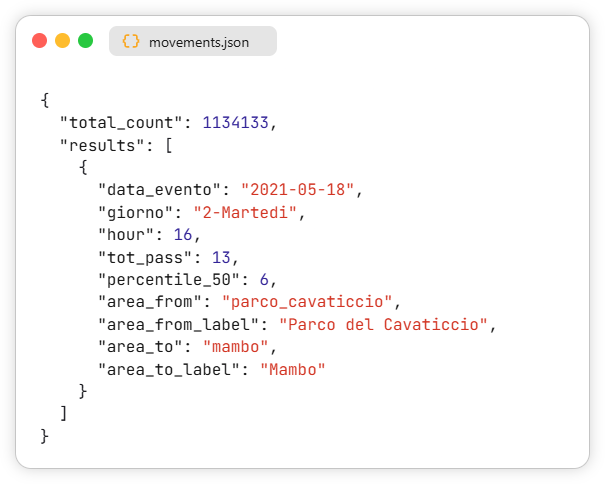
\includegraphics[width=\textwidth]{movements}
    \caption[Struttura dei dati sugli spostamenti]{Dati relativi agli spostamenti, in formato JSON, riferiti ai movimenti da Parco del Cavaticcio a Mambo, alle ore 16 del 18 maggio 2021.}
    \label{fig:movements}
\end{figure}

Tali spostamenti sono direzionati, quindi uno spostamento dalla Biblioteca Salaborsa a Palazzo D'Accursio verrà registrato separatamente da quello effettuato, inversamente, da Palazzo D'Accursio a Biblioteca Salaborsa. Anche in questo caso, entrambe le direzioni degli spostamenti sono indipendenti l'una dall'altra, e non è detto che esistano entrambe in una certa ora. Per esempio, potremmo avere una direzione in cui si spostano 100 persone (o meglio, dispositivi), mentre nell'altra se ne spostano 0 o comunque una quantità trascurabile ai fini del rilevamento dati di BolognaWiFi, quindi in entrambi questi ultimi due casi non verrebbe creata nessuna nuova entrata sul database di Open Data. A giudicare dai dati, il limite minimo necessario per creare un'entrata sul database è stato fissato in una quantità di 10 persone, in quanto non esistono spostamenti aventi valore minore. Questo aiuta anche a garantire la privacy degli utenti, in quanto se venissero pubblicati i dati di un singolo dispositivo in una certa direzione il diritto alla privacy potrebbe venire violato.

\subsection{Affollamento e Affluenza}
Considerando i dati ottenuti dalle API degli Open Data forniti dal Comune di Bologna, possiamo notare come sia affollamento che affluenza contengono entrambi dei dati aventi una struttura molto simile tra loro. Di conseguenza, questo significa che possiamo trattarli insieme, semplificando la loro gestione ed evitando di complicarla con duplicati inutili di dati.

Per entrambi viene registrata una nuova entrata per ogni ora del giorno, in ciascuna zona di Bologna coperta dal servizio BolognaWiFi. Per riuscire a garantire la privacy degli utenti, per affollamento e affluenza viene creata una nuova entrata oraria avente valore diverso da 0 solo qualora vi siano stati abbastanza utenti ad essere rimasti o entrati in una certa zona, rispettivamente per affollamento e affluenza. In caso contrario, viene comunque creata una nuova entrata, tuttavia essa avrà valore impostato a 0 di default. Questo limite minimo, a giudicare dai dati, è stato fissato in 10 persone, dato che non esiste alcun valore registrato nel range tra 1 e 9, garantendo così una completa anonimizzazione dei dati.

\begin{figure}[H]
    \centering
    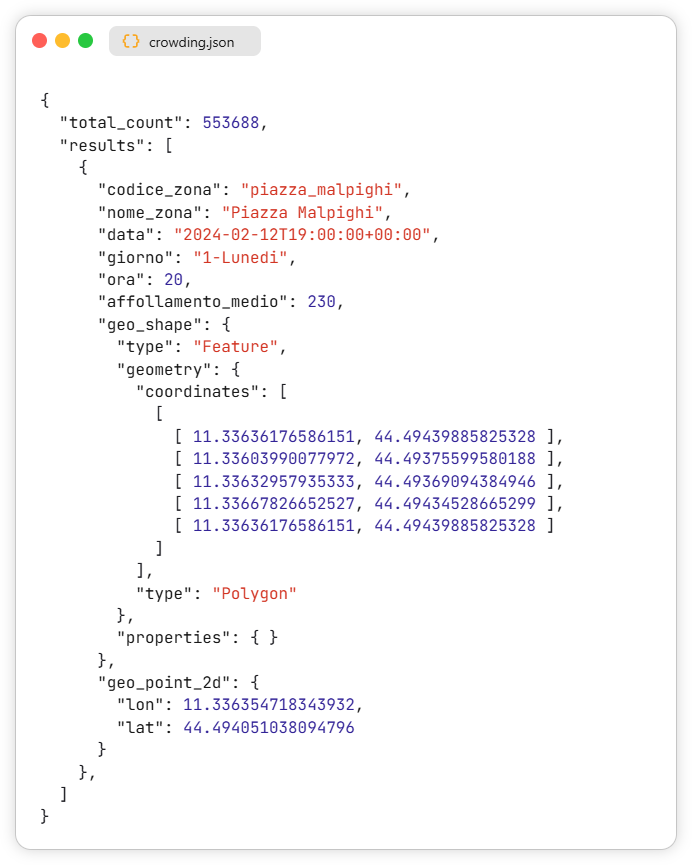
\includegraphics[width=\textwidth]{crowding}
    \caption[Struttura dei dati sull'affollamento]{Dati riguardanti l'affollamento, in formato JSON, riferiti a Piazza Malpighi alle ore 20 del 12 febbraio 2024. Notare l'attributo \textit{ora} che viene incluso nel timestamp di \textit{data} in fuso orario UTC.}
    \label{fig:crowding}
\end{figure}

\begin{figure}[H]
    \centering
    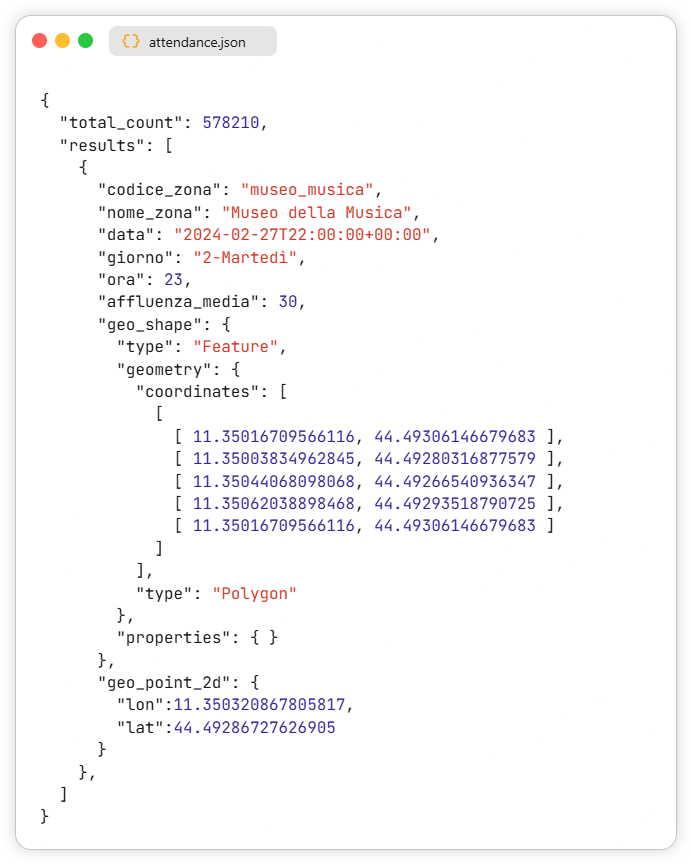
\includegraphics[width=\textwidth]{attendance}
    \caption[Struttura dei dati sull'affluenza]{Dati riguardanti l'affluenza, in formato JSON, riferiti al Museo della Musica, alle ore 23 del 27 febbraio 2024. Notare l'attributo \textit{ora} che viene incluso nel timestamp di \textit{data} in fuso orario UTC.}
    \label{fig:attendance}
\end{figure}

\section{Struttura del database}
La struttura dei dati ottenuti dall'interrogazione delle API, così come possiamo vedere in Figura~\ref{fig:movements}, Figura~\ref{fig:crowding} e Figura~\ref{fig:attendance}, è abbastanza semplice di per sé. Tuttavia, tale semplicità nasconde dei problemi di gestione delle ridondanze quando vengono salvati i dati su database, ciò avviene per svariati motivi che ora approfondiremo.

\subsection{Aree}
Innanzitutto, le informazioni relative alle aree e coordinate sono salvate in maniera differente nei tre dataset. Negli spostamenti si collegano solo i nomi e gli identificatori di ciascuna area attinente al vettore movimento, mentre sia in affollamento che in affluenza vengono specificate anche le relative coordinate del poligono, insieme a quelle del suo centroide.

Questo comporta fin da subito la necessità di creare un'entità per le aree e una separata per ciascuna coordinata, in quanto ogni poligono ha un numero variabile di punti. In questo modo non solo rimuoviamo la ridondanza tra affollamento e affluenza, ma permettiamo anche di collegare due poligoni a ciascuno spostamento, uno di partenza e uno di arrivo, cosa che non sarebbe possibile se non avessimo aggregato i tre dataset.

Notiamo subito che tale accortezza è possible solamente perché tutti e tre i dataset afferiscono alle stesse aree, ovvero i poligoni, delimitati dalla copertura del segnale di BolognaWiFi, quindi il loro dominio delle aree è completamente sovrapponibile.

\subsection{Spostamenti}
In questo modo, abbiamo assegnato un poligono di partenza e uno di arrivo a ciascuno spostamento. Rimane tuttavia il fatto che esista un numero \( n \) di spostamenti giornalieri, con \( n \leq 24 \), quindi al momento avremmo un numero esageratamente alto di entrate su database, che diventerebbe un problema in termini di richieste al server per visualizzare i dati giornalieri.

Questo problema può essere efficacemente risolto aggregando tutti i dati giornalieri: per fare ciò, fissata un'area di partenza e una di arrivo per una precisa data, creiamo 24 colonne per l'attributo \textit{percentile\_50} e altrettante 24 per \textit{tot\_pass}. In questo modo ottimizziamo il recupero dei dati effettuato dal client mediante richieste server, riducendo il numero di chiamate fino a 24 volte: basta semplicemente scaricare tutti i dati di un giorno, e utilizzarli fino a quando l'utente non chiama i dati di un altro giorno.

Riguardo al significato degli attributi, \textit{tot\_pass} è il numero di passeggeri che transitano da una zona A a una zona B nell'arco di un'ora in un determinato giorno. Invece, \textit{percentile\_50} è il mediano di tutti i \textit{tot\_pass} calcolati per tutti i giorni a una determinata ora, fino al giorno in cui vengono salvati i dati sul database di Open Data.

In questo caso, l'aggregazione dei dati è semplice perché nel dataset, nessun giorno ha un numero di entrate superiore a 24, cosa non scontata considerando che il cambio dell'ora genera un giorno con 23 ore in primavera e uno con 25 in autunno. Tale affermazione è affidabile in quanto la registrazione dei dati sugli spostamenti è cominciata l'1 aprile 2021.

\subsection{Affollamento e Affluenza}
Ancora una volta, questi due dataset si rivelano simili: avendo un insieme di attributi molto simili e lo stesso set di coordinate dei poligoni, basta scegliere uno qualunque dei due dataset per popolare le tabelle di area e coordinate che abbiamo visto prima.

In questo modo, entrambe le sezioni di \textit{geo\_shape} e \textit{geo\_point\_2d} vengono assorbite in area e coordinate, alleggerendo la struttura delle tabelle di affollamento e affluenza che andremo a realizzare. Possiamo notare che tutti i dati relativi ad affollamento e affluenza hanno un \textit{"type": "Feature"} e \textit{"type": "Polygon"}, che possono essere tranquillamente ignorati essendo uguali in tutto il dataset.

Anche qui, per ottimizzare le richieste al server nello stesso modo che abbiamo visto per gli spostamenti, aggreghiamo le 24 ore dello stesso giorno all'interno della stessa entrata, ma non solo: data la loro somiglianza, affollamento e affluenza possono essere aggregati all'interno della stessa tabella. Questo è possibile perché entrambe le loro entrate riguardano tutte le aree di Bologna ad ogni ora del giorno, quindi il numero totale è sempre uguale.

Tuttavia, in questo caso in entrambi i dataset vi sono giorni con 23 o 25 entrate giornaliere, a causa del cambio dell'ora. Tale problema si risolve facilmente, considerando che tutti gli eccessi hanno valori nulli: in caso di conflitto, basta tenere il valore massimo, in quanto uno dei due è per forza zero, mentre in caso di deficit basta assegnare 0 come valore al dato mancante.

Inoltre, sorge un ulteriore problema iniziale dovuto al fatto che i dati di affluenza sono disponibili a partire dal 1 gennaio 2024, mentre quelli riguardanti l'affollamento cominciano dal 15 gennaio 2024. Ancora una volta si risolve semplicemente assegnando uno 0 ai valori mancanti, ovvero a tutti quelli nelle due settimane in cui non vi sono dati riguardanti l'affollamento.

\subsection{Raggruppamento dei dati giornalieri}
Tutti i dati relativi allo stesso giorno vengono raggruppati all'interno della stessa riga a database, permettendo di ridurre il numero di queries che vengono effettuate al server e migliorando così le performance dell'applicazione.

Per i movimenti, non essendoci conflitti relativi al cambio dell'ora, ogni dato viene salvato in base all'attributo \textit{ora} degli Open Data, quindi uno spostamento relativo alle ore 16 salverà i passeggeri totali nell'attributo giornaliero \textit{tot\_pass\_16} e i passeggeri mediani in \textit{percentile\_50\_16}. L'orario salvato a database è quindi in fuso orario GMT+1 durante l'ora solare, mentre durante l'ora legale diventa GMT+2, seguendo quindi il fuso orario locale.

Una considerazione analoga viene effettuata per i dati di affollamento e affluenza, con la differenza che qui l'attributo \textit{ora} degli Open Data non è utilizzabile come identificatore dell'attributo in quanto viene influenzato dal cambio dell'ora. Questo si risolve facilmente utilizzando l'orario definito all'interno del timestamp \textit{data} ottenuto dagli Open Data, mediante parsing della stringa, in quanto viene specificato sempre seguendo il fuso orario UTC. In questo modo, affollamento e affluenza vengono sempre salvati in GMT, a prescindere dal fuso orario locale.

\subsection{Schema finale}
Dopo tutte le precedenti considerazioni, riportiamo in Figura~\ref{fig:database} lo schema finale del database. Per evitare di ottenere un database enorme in termini di spazio su disco, abbiamo prestato particolare attenzione ad utilizzare la quantità di memoria minore possibile per ogni attributo delle tabelle.

In particolare, considerando che gli spostamenti (sia totali che mediani), l'affollamento e l'affluenza orari raggiungono valori sempre interi che non superano mai la quantità di 10~000 e non sono mai inferiori a zero. Di conseguenza, possiamo utilizzare un tipo di dato \textit{unsigned short} senza avere timori relativi ad un possibile overflow, anzi possiamo mantenere pure una certa quantità di margine, occupando solo 2 bytes per numero, dimezzando lo spazio richiesto in confronto ai 4 bytes occupati da un normale \textit{unsigned int}.

Inoltre, una simile considerazione può essere effettuata per i numeri decimali relativi alle coordinate dei punti dei poligoni, in quanto vi sono sempre due cifre intere e 14 o 15 cifre decimali. Riguardo alle due cifre intere, possiamo utilizzarne sempre due solamente considerando la posizione geografica di Bologna, in quanto se la latitudine non rappresenta un problema, la longitudine talvolta può assumere valori a tre cifre intere in base alla posizione sulla Terra. In questo modo, su MySQL gli viene assegnato il tipo di dato \textit{decimal(17,15)}, con 15 cifre decimali su 17 cifre totali, escludendo la virgola.

\begin{figure}[H]
    \centering
    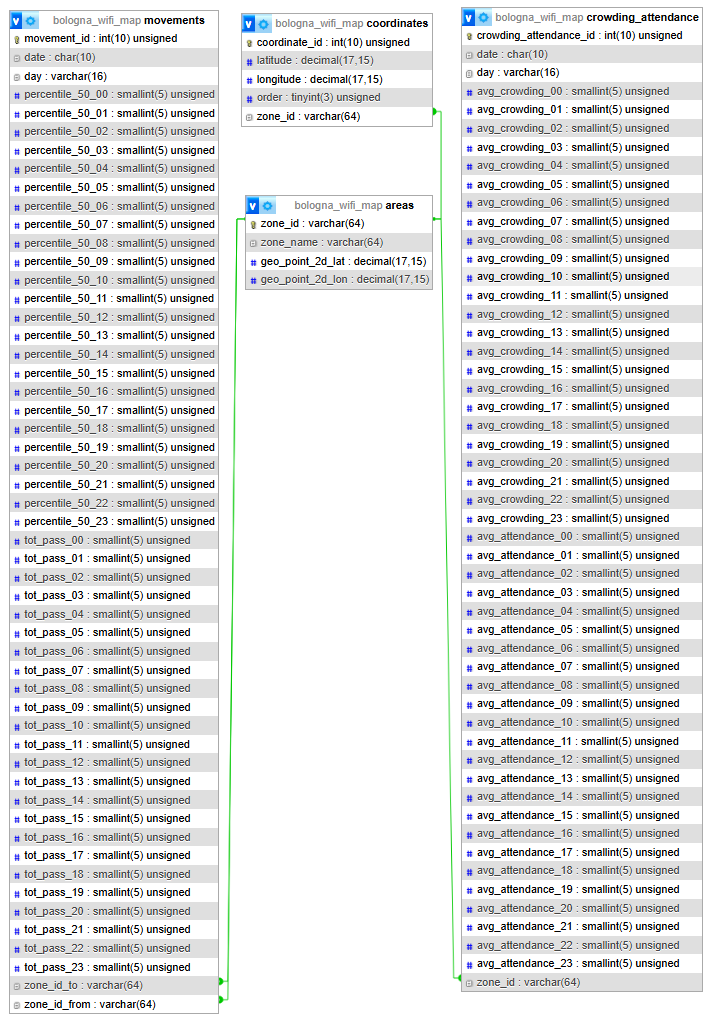
\includegraphics[width=\textwidth]{database.png}
    \caption[Schema del database]{Schema del database di BolognaWiFiMap. Notare la lista di attributi definiti per ciascuna ora.}
    \label{fig:database}
\end{figure}

\section{Connessione tra frontend e backend}
Dopo aver installato Vue.js e creato il progetto utilizzando Vite, ovvero un plugin di Vue per la nuova sintassi SFC (Single-File Components), abbiamo impostato l'indirizzo e la porta del server nel file di configurazione \Verb_vite.config.js_, settandolo a 0.0.0.0 per permettere al frontend di comunicare col backend indipendentemente dall'indirizzo del server, che in questo caso si riferisce a quello del server Apache. Inoltre, abbiamo specificato l'alias \Verb_@_ per definire la directory \Verb_./src/frontend_, semplificando il percorso dei file da importare.

\begin{figure}[H]
    \centering
    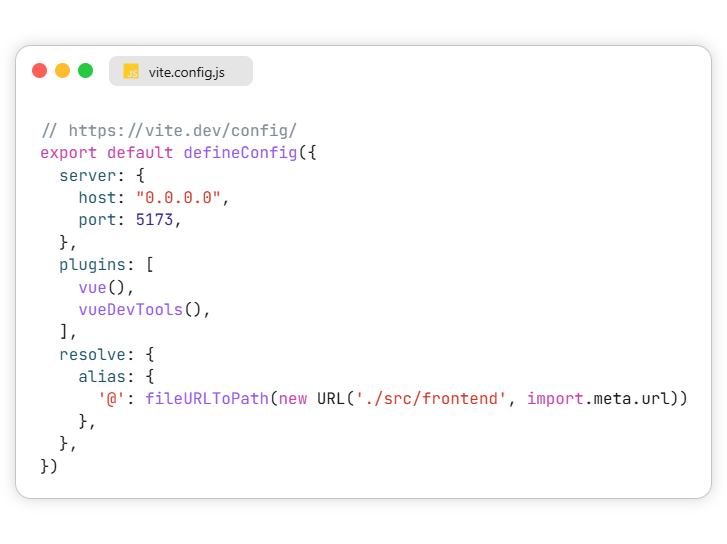
\includegraphics[width=\textwidth]{vite_config}
    \caption[Configurazione delle impostazioni Vite]{Configurazione delle impostazioni Vite relative al progetto Vue, dove si definiscono in particolare l'indirizzo e la porta per accedere al server.}
    \label{fig:vite_config}
\end{figure}

\section{Single-Page App}
Questa applicazione è stata realizzata seguendo il modello della \textit{Single-Page App}, ovvero una sola pagina web che carica selettivamente i suoi componenti o aggiorna i suoi dati senza necessità di ricaricare la pagina. Questo è permesso sia dallo stesso framework Vue.js, sia dall'implementazione di richieste AJAX che il client effettua al server.

\section{Implementazione richieste AJAX}
Le richieste AJAX sono effettuate in modo asincrono dal client al server per ottenere dei dati che verranno utilizzati per aggiornare la pagina, evitando di dover effettuare un ricaricamento della stessa. Per la sua implementazione abbiamo utilizzato la funzione \Verb_fetch()_ built-in di JavaScript, creando tre funzioni per aggiornare rispettivamente le aree, con \Verb_fetchAreas()_, gli spostamenti, con \Verb_fetchMovements()_, e infine l'affollamento insieme all'affluenza, con \Verb_fetchCrowdingAttendance()_. 

Abbiamo definito tutte queste funzioni nel file \Verb_api.js_, essendo molto semplici riportiamo in Figura~\ref{fig:ajax_api_movements} solo quella relativa agli spostamenti. In particolare, queste custom API utilizzano l'indirizzo corrente comprensivo di porta, per poi appendere a tale stringa l'url specifico dell'API a cui si vuole effettuare la richiesta. Si noti come questo setup presuppone un deployment di frontend e backend sullo stesso server, o quantomeno di un ridirezionamento tramite proxy di tali richieste effettuate a frontend verso l'url appropriato del backend, se dovessero essere in deployment su server diversi.

\begin{figure}[H]
    \centering
    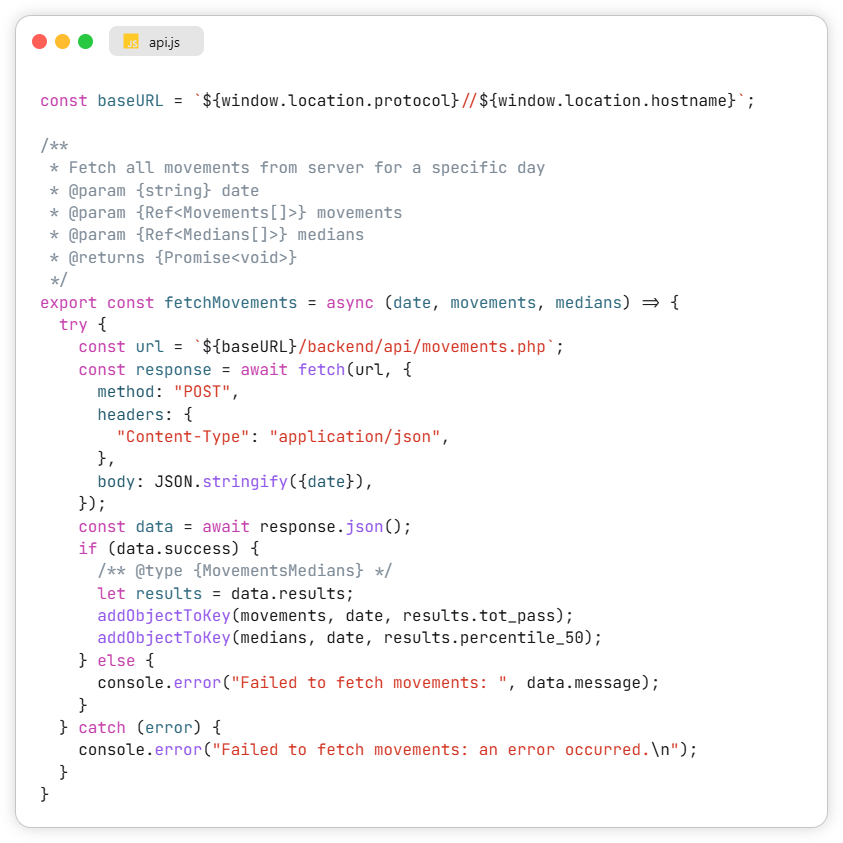
\includegraphics[width=\textwidth]{ajax_api_movements}
    \caption[Richiesta AJAX per ottenere la lista dei movimenti]{Implementazione di una funzione che effettua una richiesta AJAX per ottenere la lista dei movimenti di una specifica data.}
    \label{fig:ajax_api_movements}
\end{figure}

\section{Popolamento del database}
Affinché le richieste AJAX possano andare a buon fine, bisogna aver popolato il database. Questo compito è svolto mediante l'esecuzione del file \Verb_updater.php_, il quale controlla l'ultima data dei dati raccolti sul database e provvede ad aggiornarli, scaricando tutti i nuovi dati.

In fase di development o test, questo script viene lanciato manualmente, ma in un futuro deployment basterebbe automatizzare la sua esecuzione utilizzando Task Scheduler su Windows o un Cron Job su Linux. Tale script, riportato in Figura~\ref{fig:updater} richiama 3 funzioni differenti per svolgere il suo compito, che qui non mostreremo per via della loro lunghezza.

\begin{figure}[H]
    \centering
    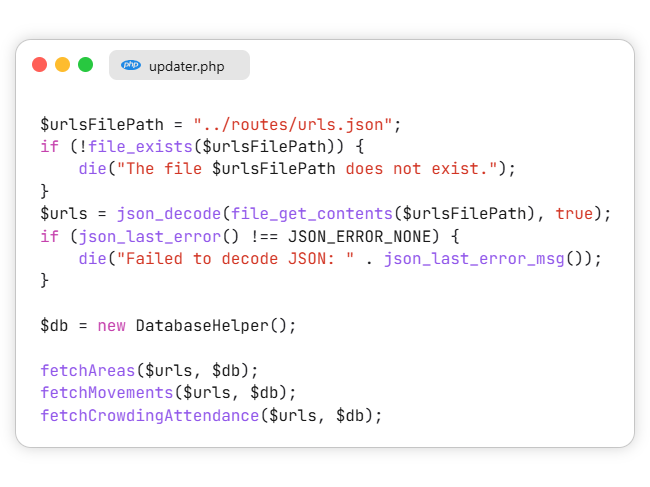
\includegraphics[width=\textwidth]{updater_noligature}
    \caption[Script per setup o aggiornamento di dati sul database]{Script che viene eseguito per effettuare il setup o per aggiornare i dati sul database, utilizzando gli url definiti in \textit{urls.json} per effettuare le chiamate alle API del sito degli Open Data di BolognaWiFi \cite{BolognaWiFi_Spostamenti,BolognaWiFi_Affollamento,BolognaWiFi_Affluenza}.}
    \label{fig:updater}
\end{figure}

Innanzitutto, viene aggiornata la lista delle aree, nel caso se ne trovino di nuove. Quindi si scaricano, in ordine, prima i movimenti, poi l'affollamento insieme all'affluenza. All'interno di entrambe le funzioni, vengono scaricati i dati giorno per giorno, fino ad arrivare agli ultimi disponibili. Tuttavia, date le limitazioni delle API offerte da BolognaWiFi, vengono scaricati al massimo 100 elementi alla volta. Questo chunk così ottenuto viene messo in coda in una lista, per poi effettuare una nuova chiamata alla stessa API riguardante lo stesso giorno, ma con un offset aumentato di 100. Le stesse API pongono un limite totale di 10~100 alla somma di offset e numero di elementi, ma considerando che in un singolo giorno non si arriva nemmeno a 2~000 elementi totali in tutti e tre i dataset, tale limite effettivo di 10~000 all'offset non è poi così restrittivo.

% \section{Funzionalità}
\section{Pagina iniziale}
Appena caricato il sito, viene visualizzata la mappa della città di Bologna insieme a tutte le aree coperte dal servizio BolognaWiFi, evidenziate come dei poligoni colorati in azzurro. Tali poligoni sono interattivi e, cliccandoli, viene mostrato un popup contenente il nome dell'area in questione. In Figura~\ref{fig:desktop_main} riportiamo uno screenshot della schermata iniziale.

\begin{figure}[H]
    \centering
    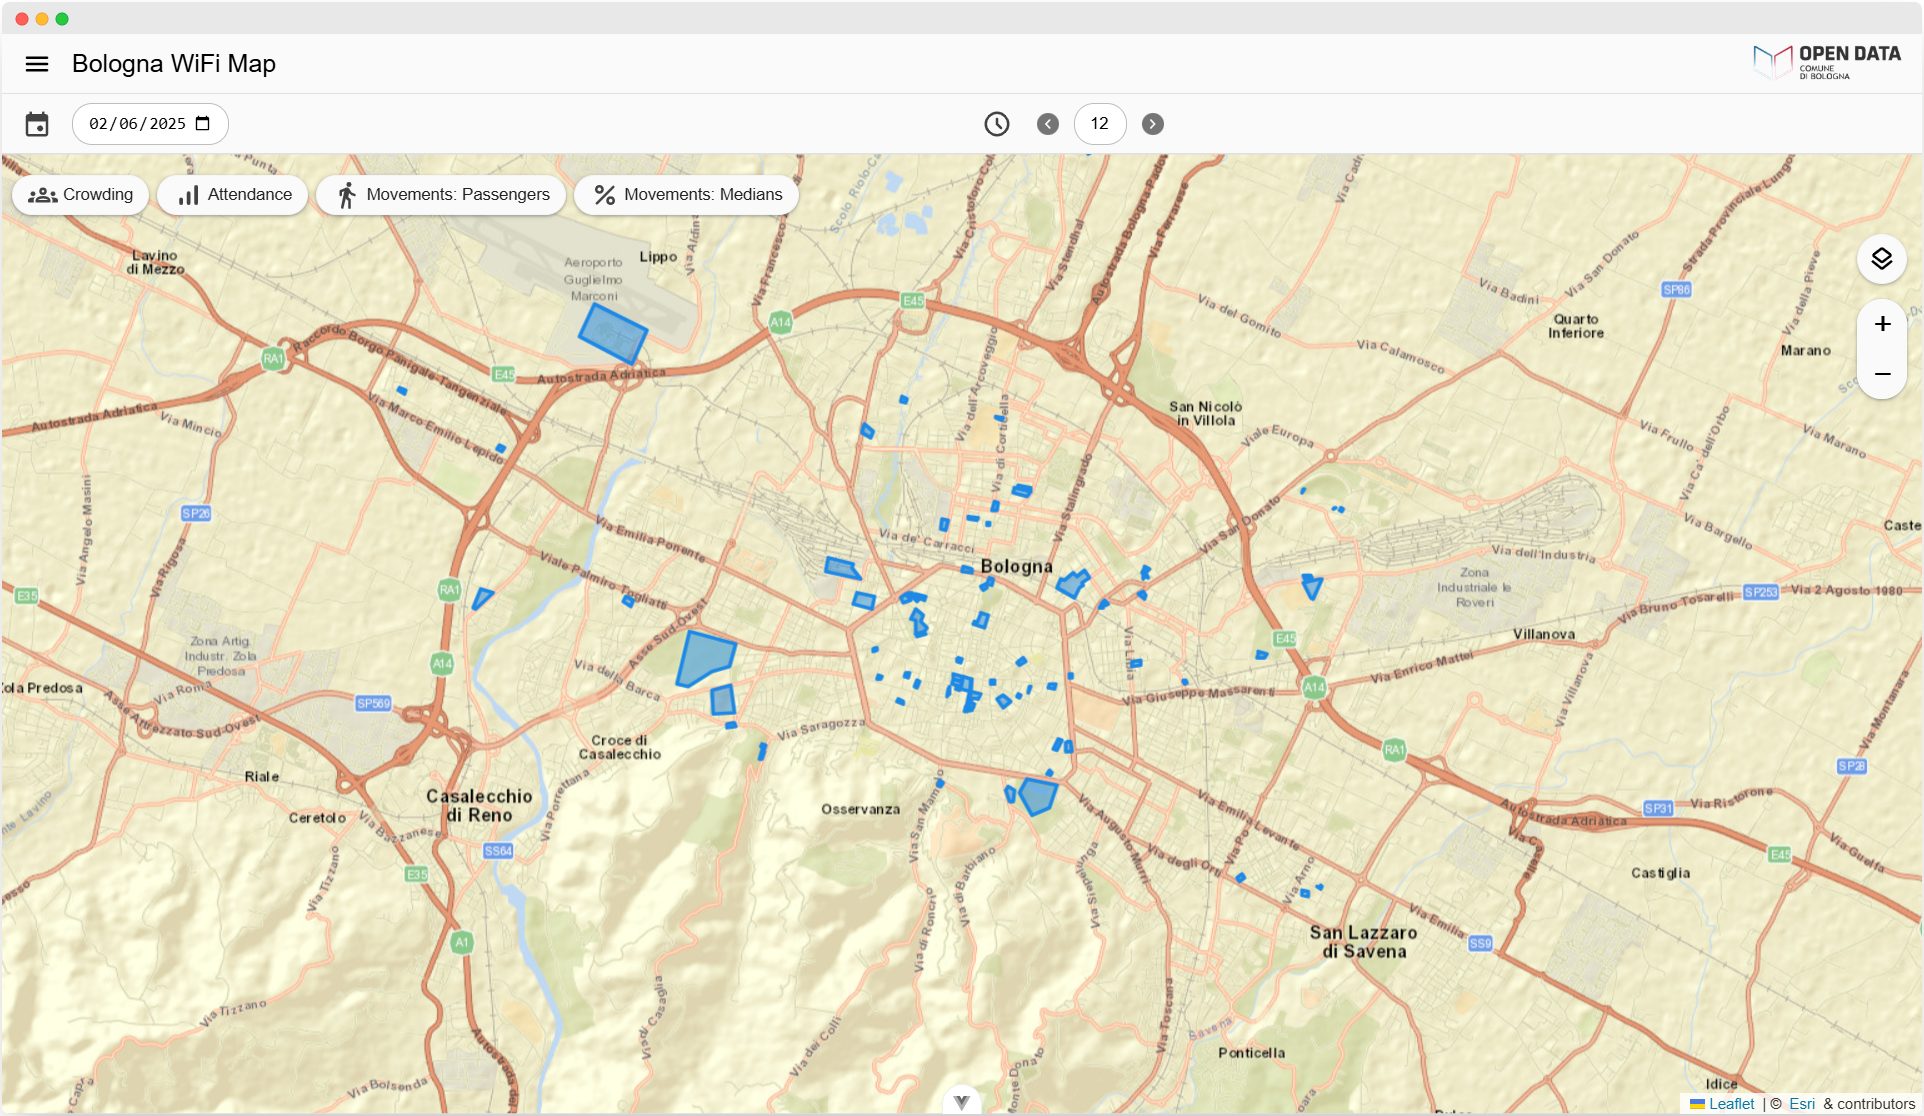
\includegraphics[width=\textwidth]{desktop_main_alt}
    \caption[Pagina iniziale su desktop]{Pagina iniziale dell'applicazione su desktop. Le aree coperte da BolognaWiFi sono indicate con dei poligoni azzurri.}
    \label{fig:desktop_main}
\end{figure}

Inoltre, dato che queste aree variano molto in termimi di dimensioni, abbiamo creato una funzione che aumenta automaticamente lo zoom della mappa ogni volta che si clicca un poligono, incrementandolo in base alla sua superficie. Questo diventa necessario per migliorare l'esperienza utente dal momento in cui un click su un poligono di grandi dimensioni è immediatamente visibile, ma un poligono piccolo è innegabilmente più difficile da individuare su una mappa senza effettuare uno zoom. Così facendo, semplifichiamo il workflow dell'utente, evitandogli di dover sempre zoommare manualmente. La libreria Leaflet applica automaticamente una transizione non appena modifichiamo lo zoom. Il risultato di tale processo è visibile in Figura~\ref{fig:zoom_desktop}

\begin{figure}[H]
    \centering
    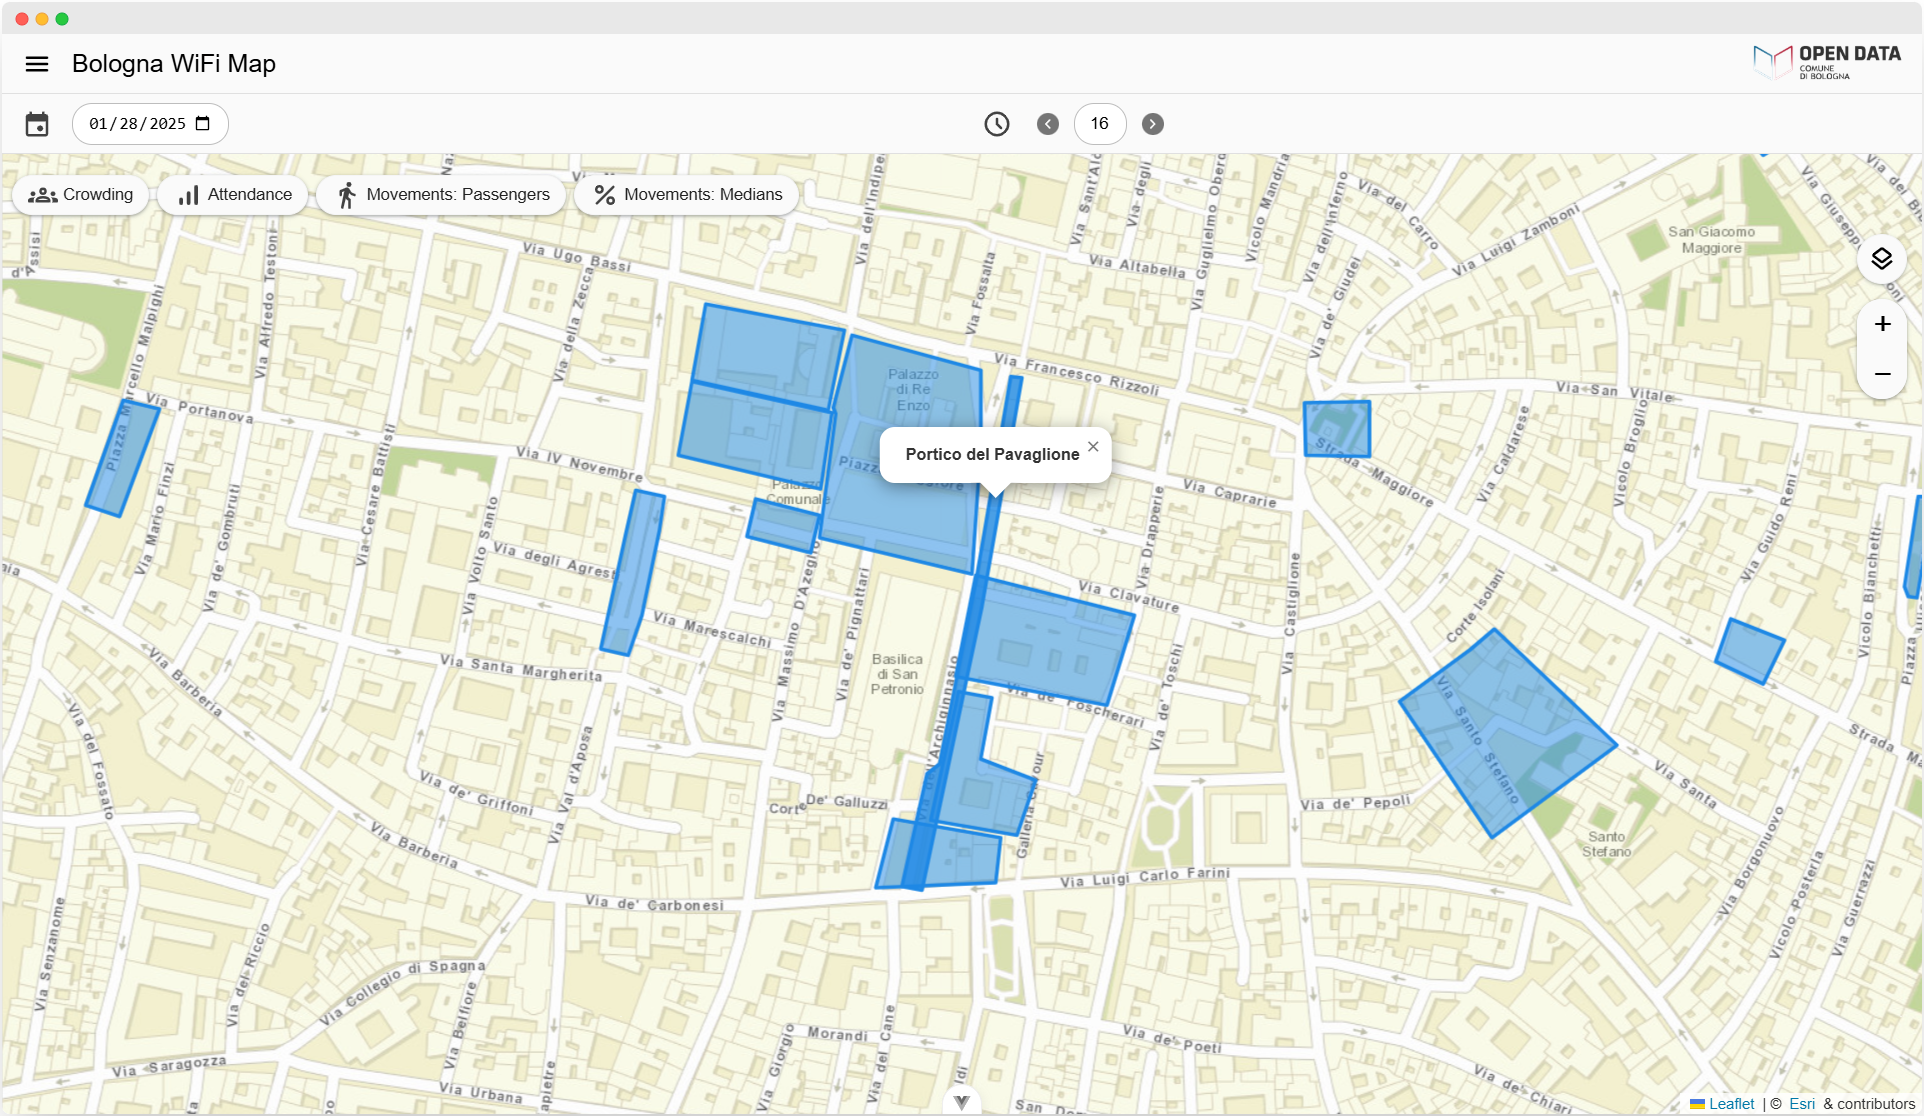
\includegraphics[width=\textwidth]{desktop_zoom}
    \caption[Zoom automatico al click di un poligono]{Zoom effettuato automaticamente al click di un poligono.}
    \label{fig:zoom_desktop}
\end{figure}

Il livello di zoom da applicare al click viene calcolato effettuando tre scaglioni di zoom in base all'estensione della superficie del poligono, categorizzandoli in grandi, medi, e piccoli. Un poligono più grande necessita di uno zoom inferiore, mentre uno piccolo andrà zoommato maggiormente, come possiamo vedere in Figura~\ref{fig:zoom_code}.

\begin{figure}[H]
    \centering
    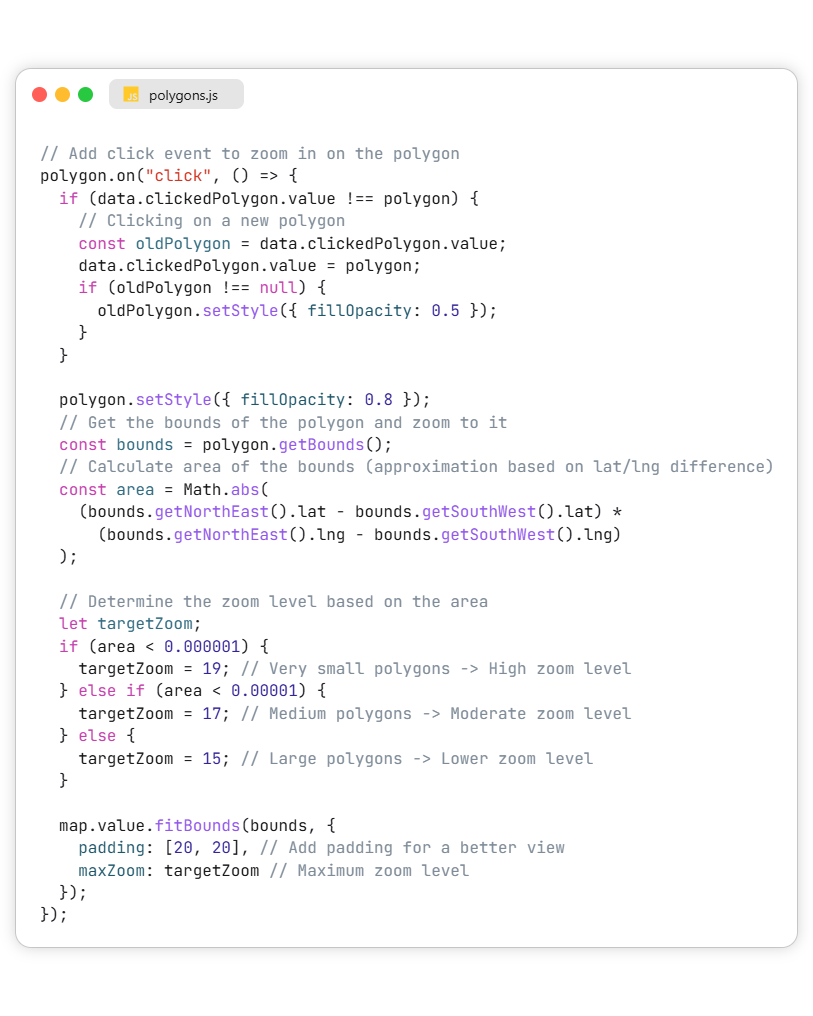
\includegraphics[width=\textwidth]{polygon_zoom}
    \caption[Codice per lo zoom al click del poligono]{Codice per calcolare il tipo di zoom del poligono e assegnarlo al click.}
    \label{fig:zoom_code}
\end{figure}

Inoltre, è possibile cambiare il tipo di mappa che si vuole visualizzare, utilizzando il bottone dei \textit{layers} posto sopra ai controlli dello zoom. Si può scegliere la vista satellite, quella del terreno o la mappa di default che visualizza le strade. Il relativo menù espanso è visibile in Figura~\ref{fig:layers}.

\begin{figure}[H]
    \centering
    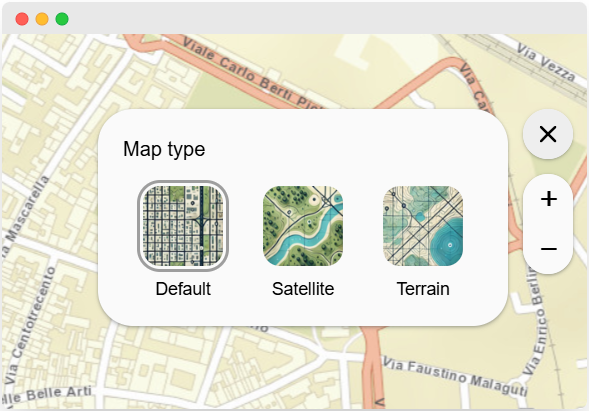
\includegraphics[width=\textwidth]{desktop_layers}
    \caption[Menù per la scelta del tipo di mappa]{Menù per effettuare la scelta del tipo di mappa da visualizzare.}
    \label{fig:layers}
\end{figure}

\section{Informazioni su una zona o spostamento}
L'applicazione permette di modificare la data e l'ora tramite gli appositi campi di input nella barra in alto. A lato del campo dell'ora vi sono due bottoni, uno a destra e uno sinistra, che permettono rispettivamente di incrementare o decrementare di un'unità l'ora corrente. Nel caso si dovesse valicare il giorno, l'applicazione gestisce automaticamente la modifica appropriata alla data, permettendo quindi una scorciatoia per uno scorrimento relativamente più veloce del tempo.

Sotto alla barra in alto troviamo quattro bottoni a forma di pillola che permettono di scegliere la visualizzazione dei dati richiesta. In ordine sono affollamento, affluenza, spostamenti totali dei passeggeri e spostamenti mediani. Vediamoli più nel dettaglio.

\subsection{Affollamento}
Scegliendo il primo bottone viene visualizzato l'affollamento relativo alla data e ora selezionate nella barra in alto, colorando i poligoni di giallo tanto di più quanto maggiore è il numero di persone che rimangono nella stessa area durante una certa ora. Cliccando su un poligono viene mostrato un popup che ne indica il valore dell'affollamento, insieme a quello massimo in assoluto, calcolato su tutto il dataset.

\begin{figure}[H]
    \centering
    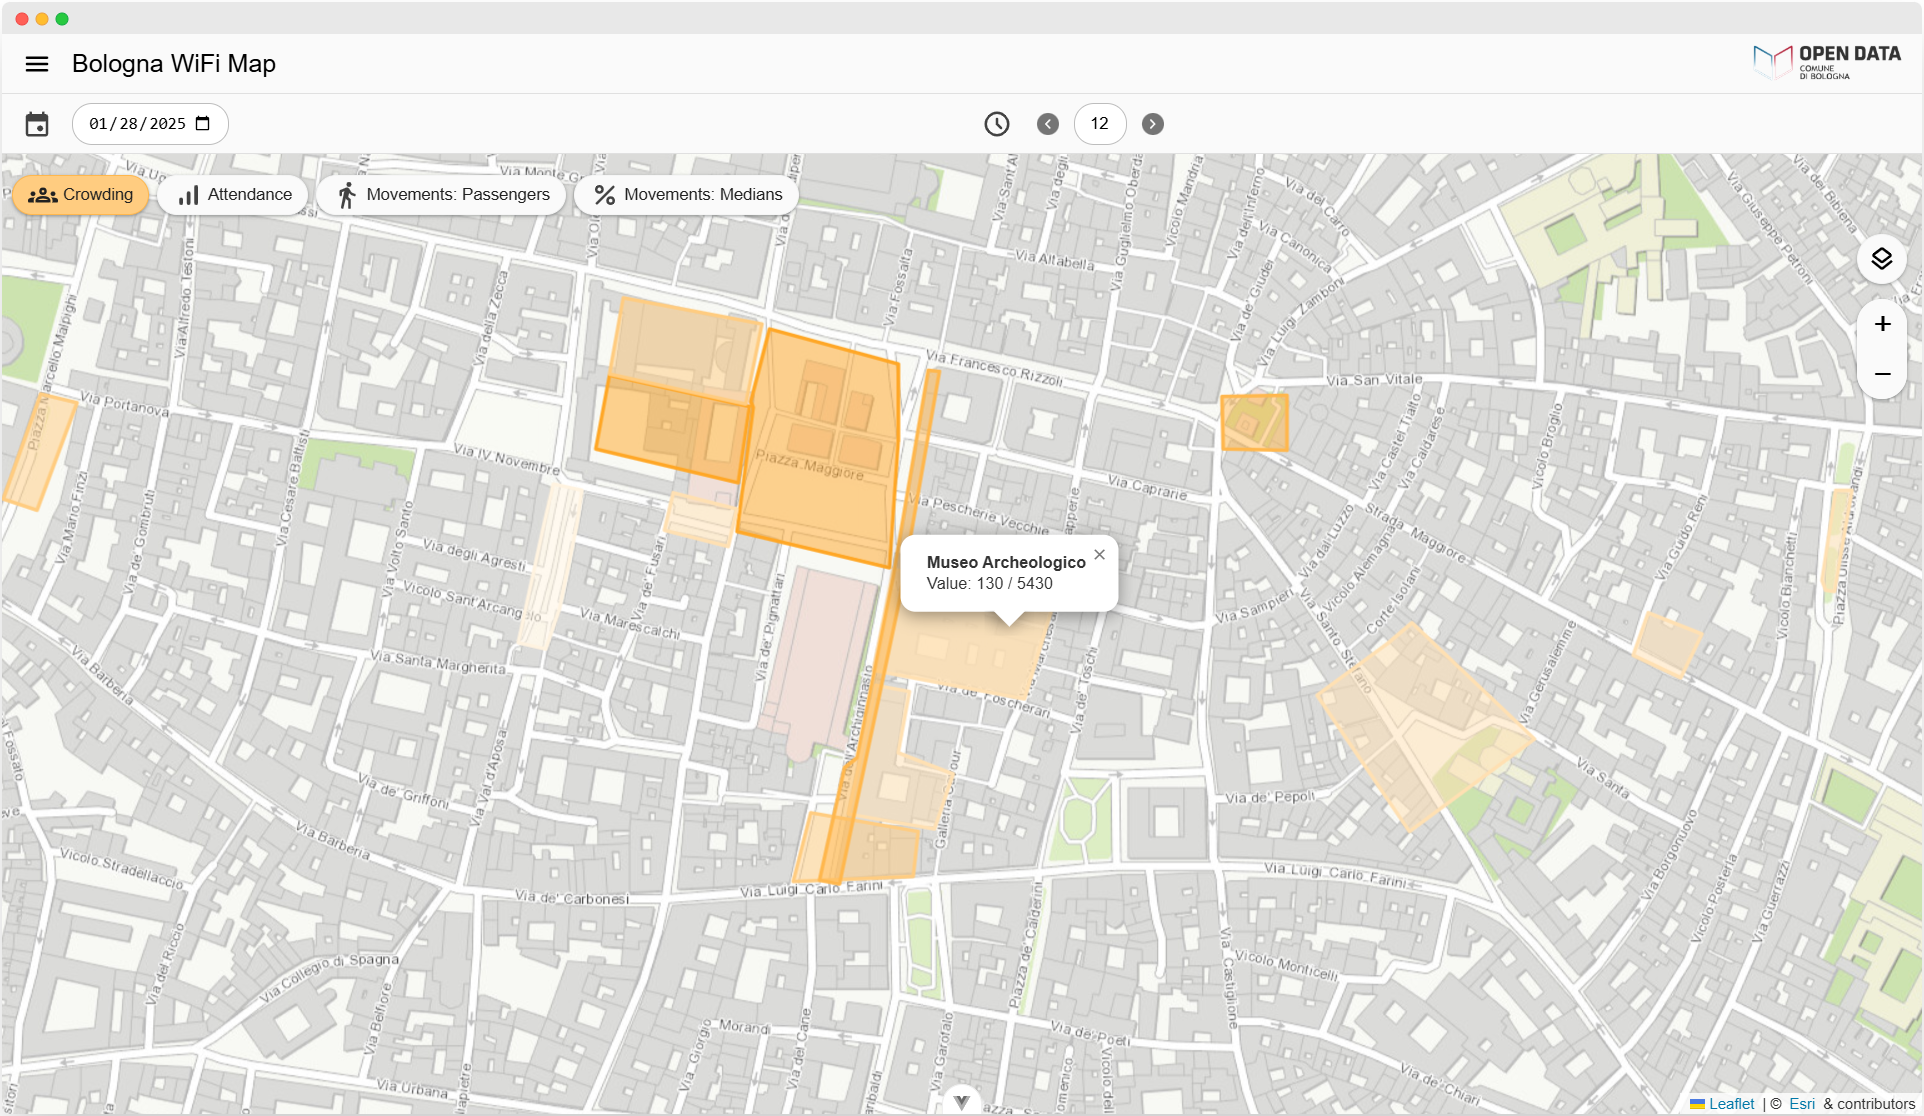
\includegraphics[width=\textwidth]{desktop_crowding}
    \caption[Screenshot dell'affollamento su desktop]{Screenshot dell'applicazione su desktop, relativo alla schermata di affollamento. Notare la barra in alto che permette di impostare la data e l'ora di cui vogliamo visualizzare i dati.}
    \label{fig:desktop_crowding}
\end{figure}

\subsection{Affluenza}
Scegliendo il secondo bottone viene visualizzata la relativa affluenza, colorando i poligoni di rosso tanto di più quanto maggiore è il numero di persone che entrano in una data area a una certa ora. Cliccando su un poligono viene mostrato un popup che ne indica il valore dell'affluenza, insieme a quello massimo in assoluto, calcolato su tutto il dataset.

\begin{figure}[H]
    \centering
    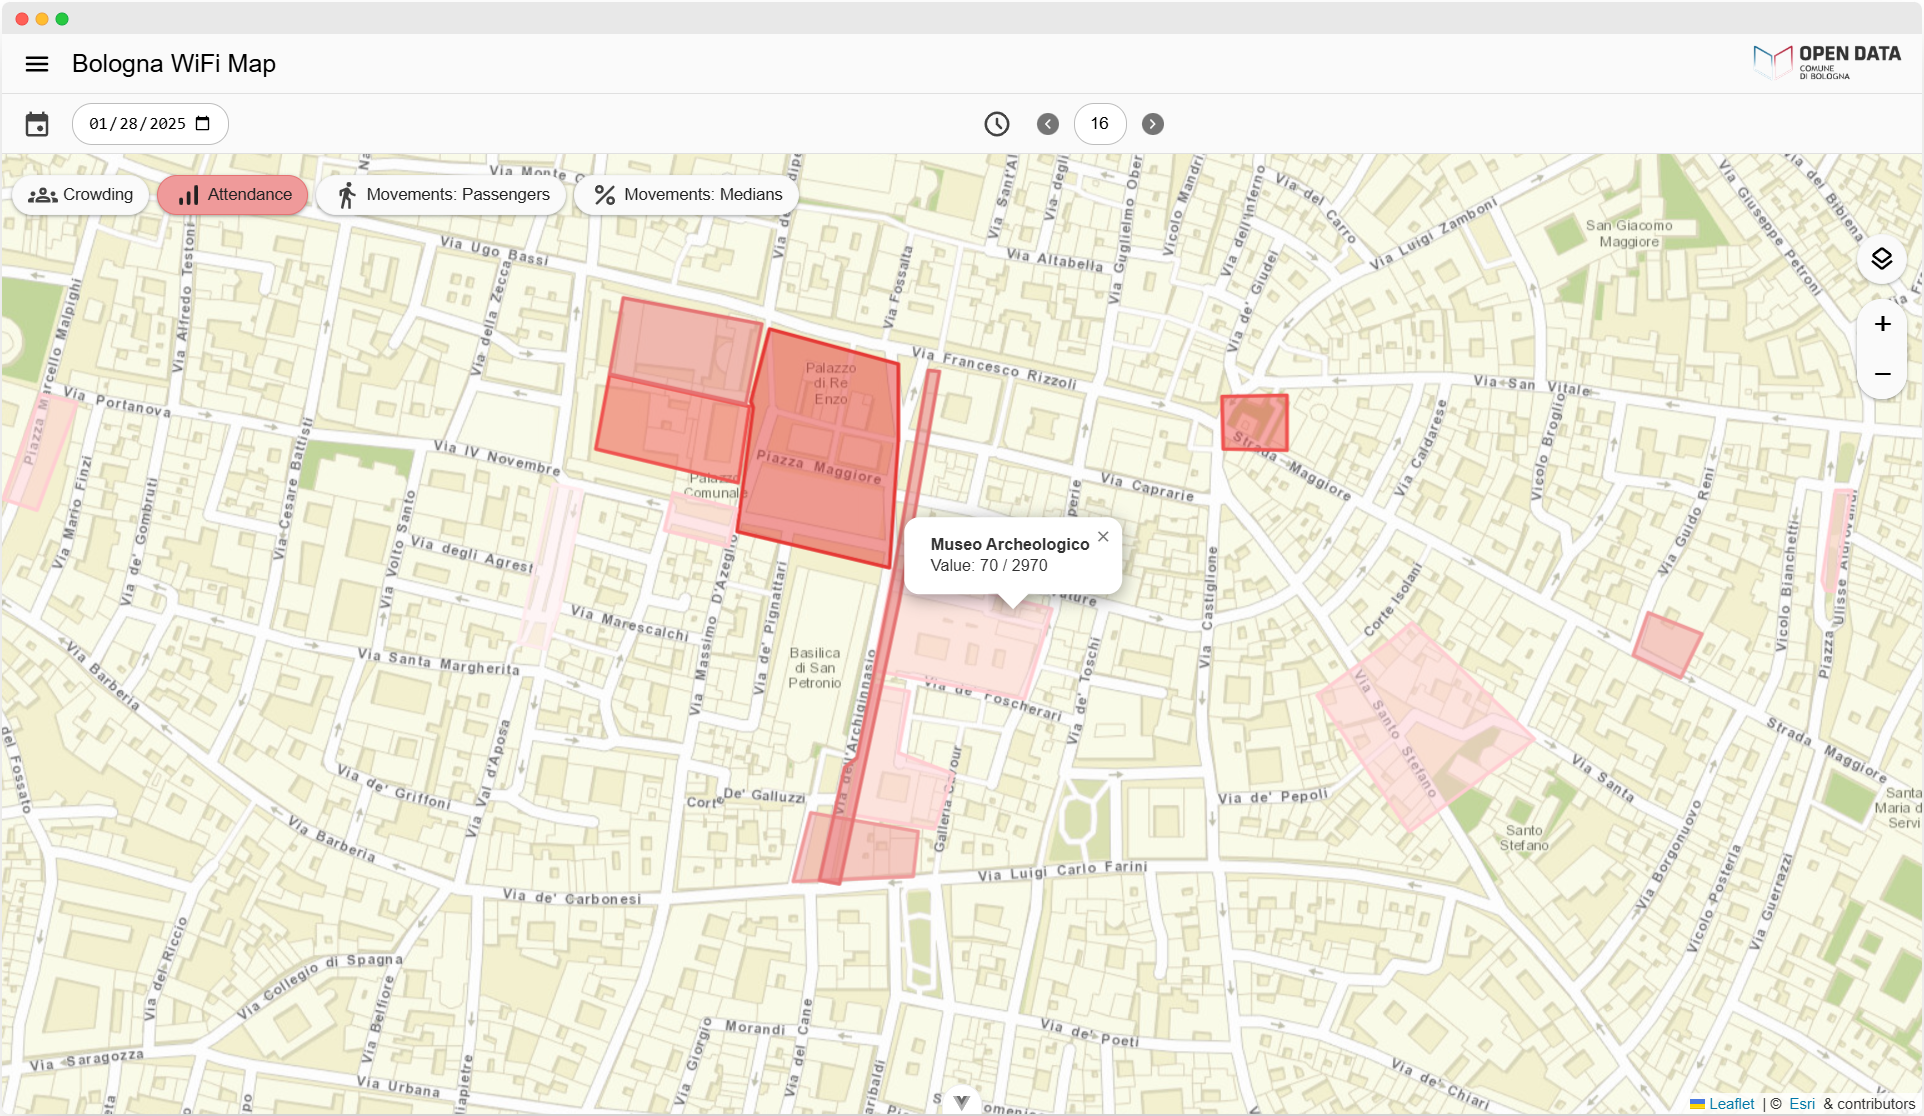
\includegraphics[width=\textwidth]{desktop_attendance}
    \caption[Screenshot dell'affluenza su desktop]{Screenshot dell'applicazione su desktop, relativo alla schermata di affluenza.}
    \label{fig:desktop_attendance}
\end{figure}

\subsection{Spostamenti}
Scegliendo il terzo bottone vengono visualizzati tutti i relativi spostamenti in termini di totale dei passeggeri, colorando tutti i poligoni di viola, mentre le linee colleganti due aree saranno colorate in viola tanto più scuro quanto maggiore è il numero di passeggeri in transito in una certa ora. Per una migliore visibilità, lo spessore delle linee è direttamente proporzionale al numero di persone che si spostano da una zona all'altra, sempre all'interno dell'ora selezionata. Cliccando su un poligono viene mostrato un popup contenente solo il nome della zona, mentre cliccando su una linea vengono mostrate le aree di origine e destinazione, insieme al valore corrente di passeggeri in transito.

\begin{figure}[H]
    \centering
    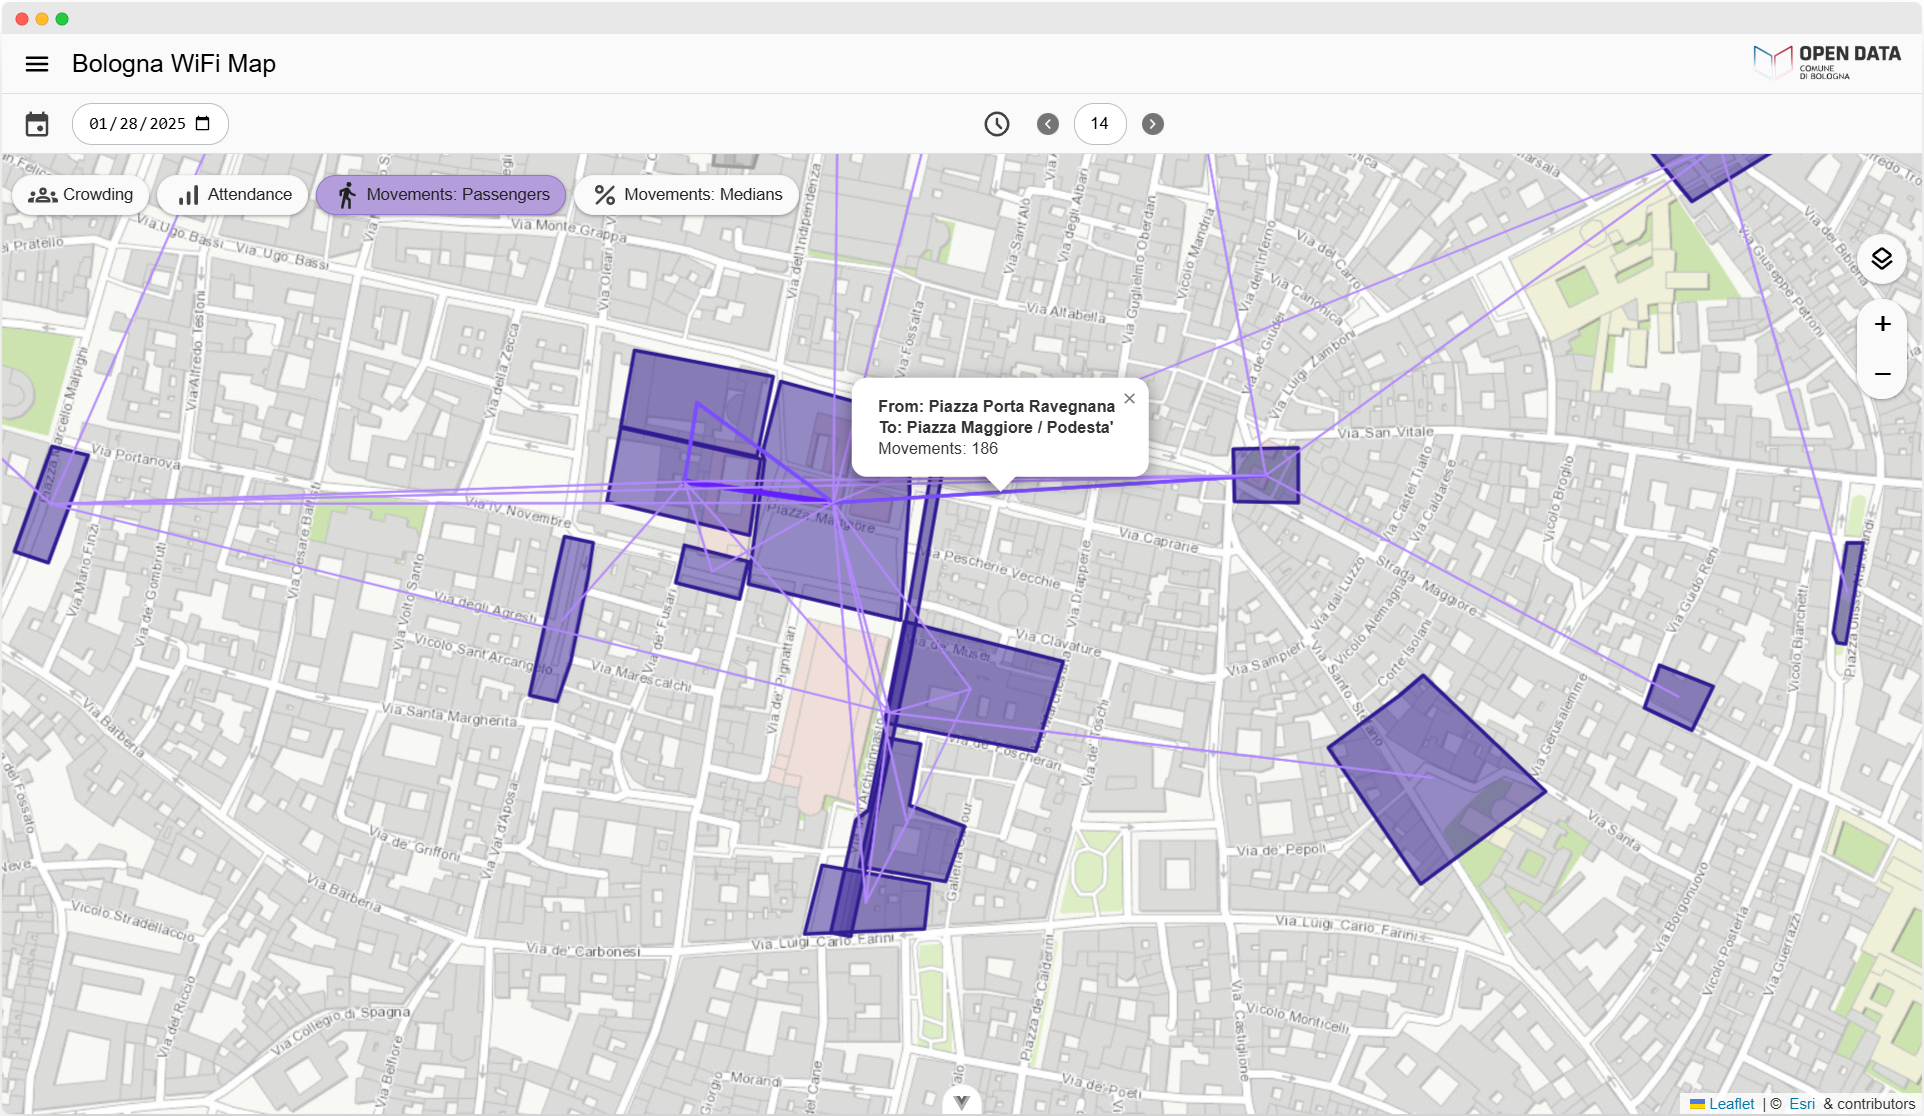
\includegraphics[width=\textwidth]{desktop_passengers}
    \caption[Screenshot degli spostamenti dei passeggeri su desktop]{Screenshot dell'applicazione su desktop, relativo alla schermata di visualizzazione degli spostamenti dei passeggeri.}
    \label{fig:desktop_passengers}
\end{figure}

Scegliendo il quarto bottone possiamo effettuare un ragionamento totalmente analogo con i dati relativi al numero mediano di passeggeri, i quali verranno visualizzati in colore fucsia. Analogamente, si applica la stessa logica per il click su poligoni e linee, con i dati relativi ai mediani.

\begin{figure}[H]
    \centering
    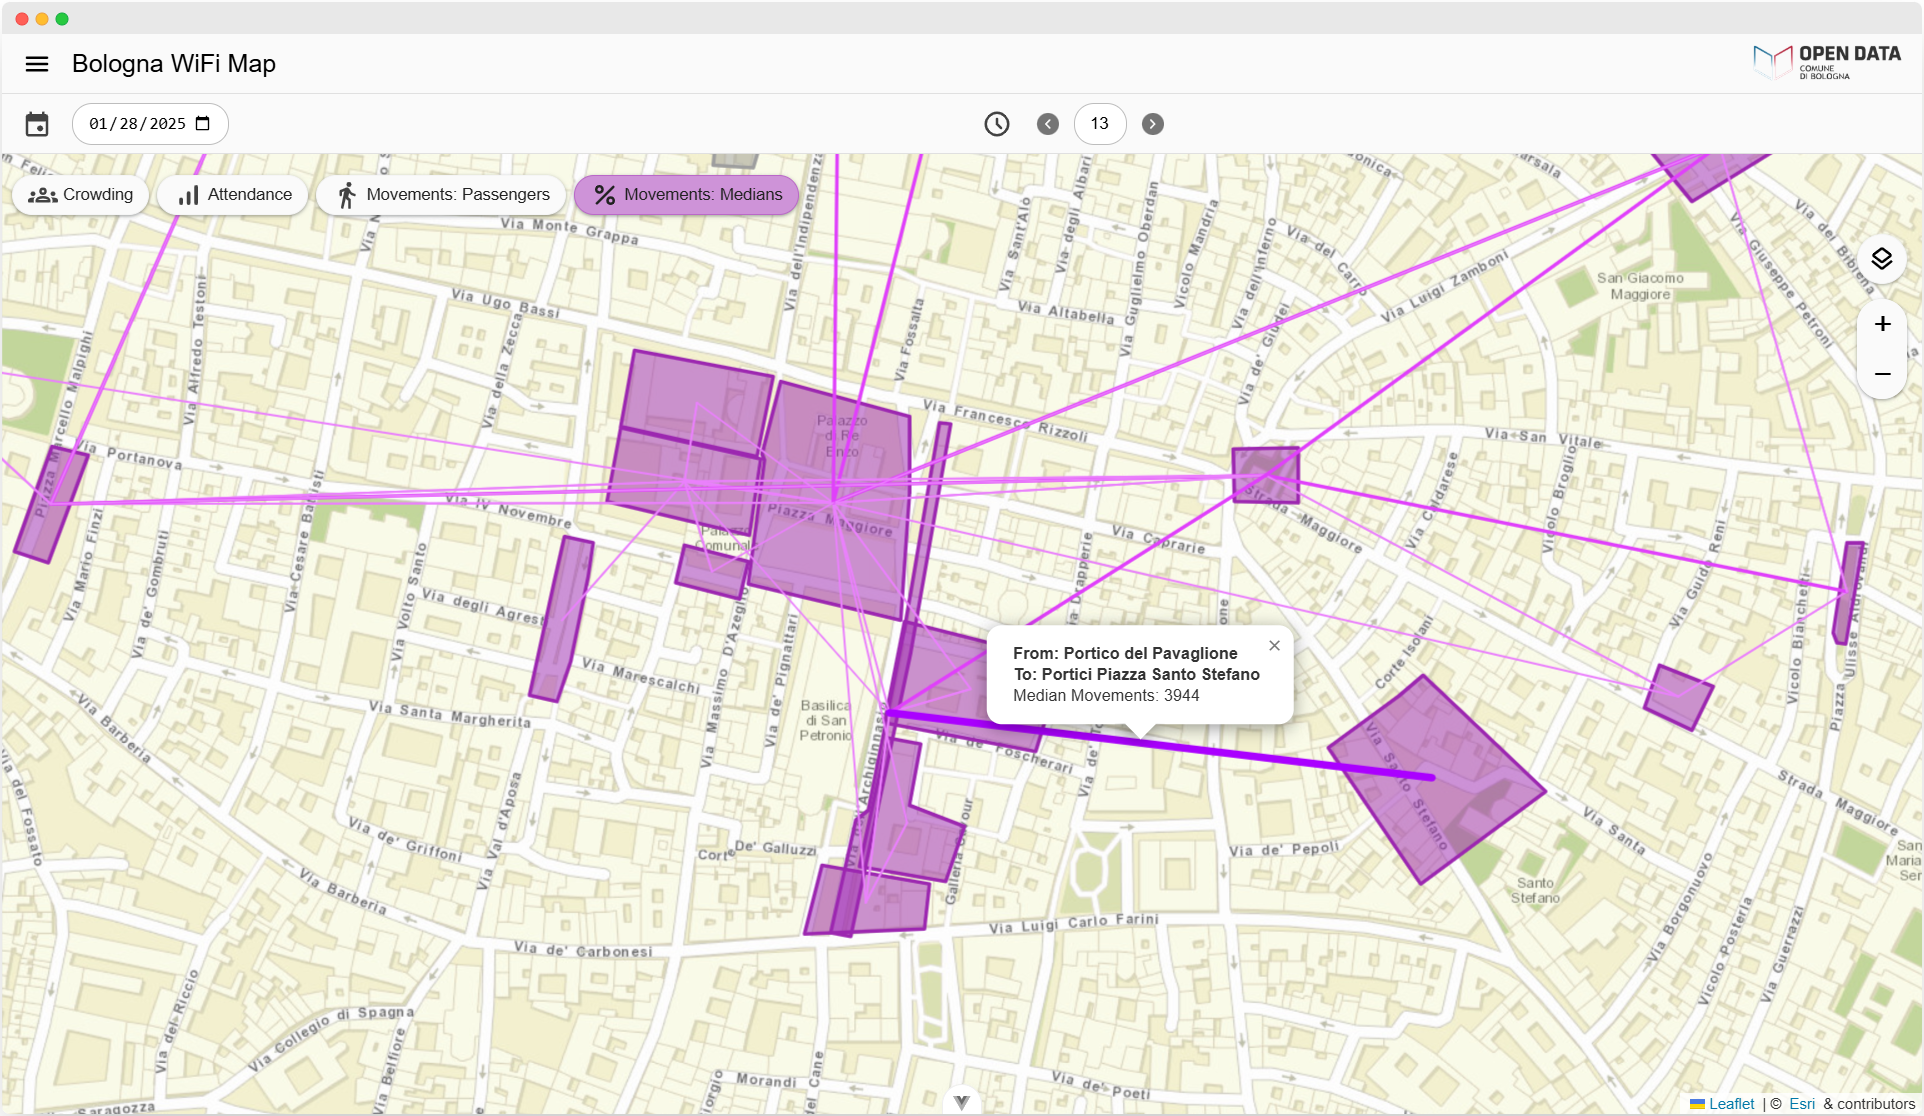
\includegraphics[width=\textwidth]{desktop_medians}
    \caption[Screenshot degli spostamenti mediani su desktop]{Screenshot dell'applicazione su desktop, relativo alla schermata di visualizzazione degli spostamenti mediani.}
    \label{fig:desktop_medians}
\end{figure}

\section{Calcolo delle opzioni di visualizzazione}
Discutere di colori sembra molto facile, ma la loro scelta è cruciale affinché la visualizzazione risulti efficace e semplice da comprendere a colpo d'occhio.

Innanziutto, consideriamo il caso di affollamento e affluenza. Tutti i dati sono concentrati nei poligoni, quindi saranno queste le entità da colorare in maniera più forte all'aumentare dei rispettivi valori.

Riguardo agli spostamenti, sia totali che mediani, possiamo notare come i poligoni non abbiano informazioni di per sé, quindi possiamo colorarli della stessa sfumatura. Invece, i dati interessanti sono contenuti all'interno delle polilinee, ovvero nelle relazioni tra due poligoni, quindi coloreremo quest'ultime in maniera tanto più scura quanto maggiore è il numero delle persone in transito da una zona all'altra. Inoltre, per evidenziare maggiormente questi dati, le abbiamo rese più spesse dove ci sia un flusso maggiore e più sottili dove tale flusso sia invece minore.

Per semplificare la visualizzazione, i poligoni aventi affollamento o affluenza nulli, insieme ai poligoni sprovvisti di spostamenti uscenti o entranti, verranno rispettivamente colorati di grigio, così da essere immediatamente riconoscibili e non confondibili con quelli che invece presentano semplicemente dei valori bassi.

Per determinare le sfumature di colori da utilizzare in ogni caso abbiamo utilizzato il codice riportato in Figura~\ref{fig:map_options_factory}, il quale innanzitutto determina se si tratta di un poligono o di una polilinea.

Per evitare un bias troppo grande nei confronti dei dati piccoli e permettere agli stessi di essere visualizzati con la giusta importanza, non abbiamo utilizzato una scala lineare bensì una pseudologaritmica, visibile in \Verb_shadeFactory()_, in cui si considera la radice quadrata del valore corrente diviso il valore massimo, così da normalizzarli in un range tra 0 e 1. I valori massimi per ciascuno delle quattro tipologie di dati sono stati salvati in un file JSON separato, così da essere facilmente accessibili e potenzialmente aggiornabili.

Una volta ottenuto il valore pseudologaritmico, si seleziona la sfumatura di colore corrispondente dall'array \Verb_shades[]_, nel caso dei poligoni, o dall'array \Verb_lineShades[]_ per le polilinee. In quest'ultimo caso, si utilizza lo stesso valore pseudologaritmico per determinare lo spessore della linea da visualizzare. Tutti i colori sono stati definiti in un file a parte, che viene richiamato così da permettere un incapsulamento migliore del codice.

\begin{figure}[H]
    \centering
    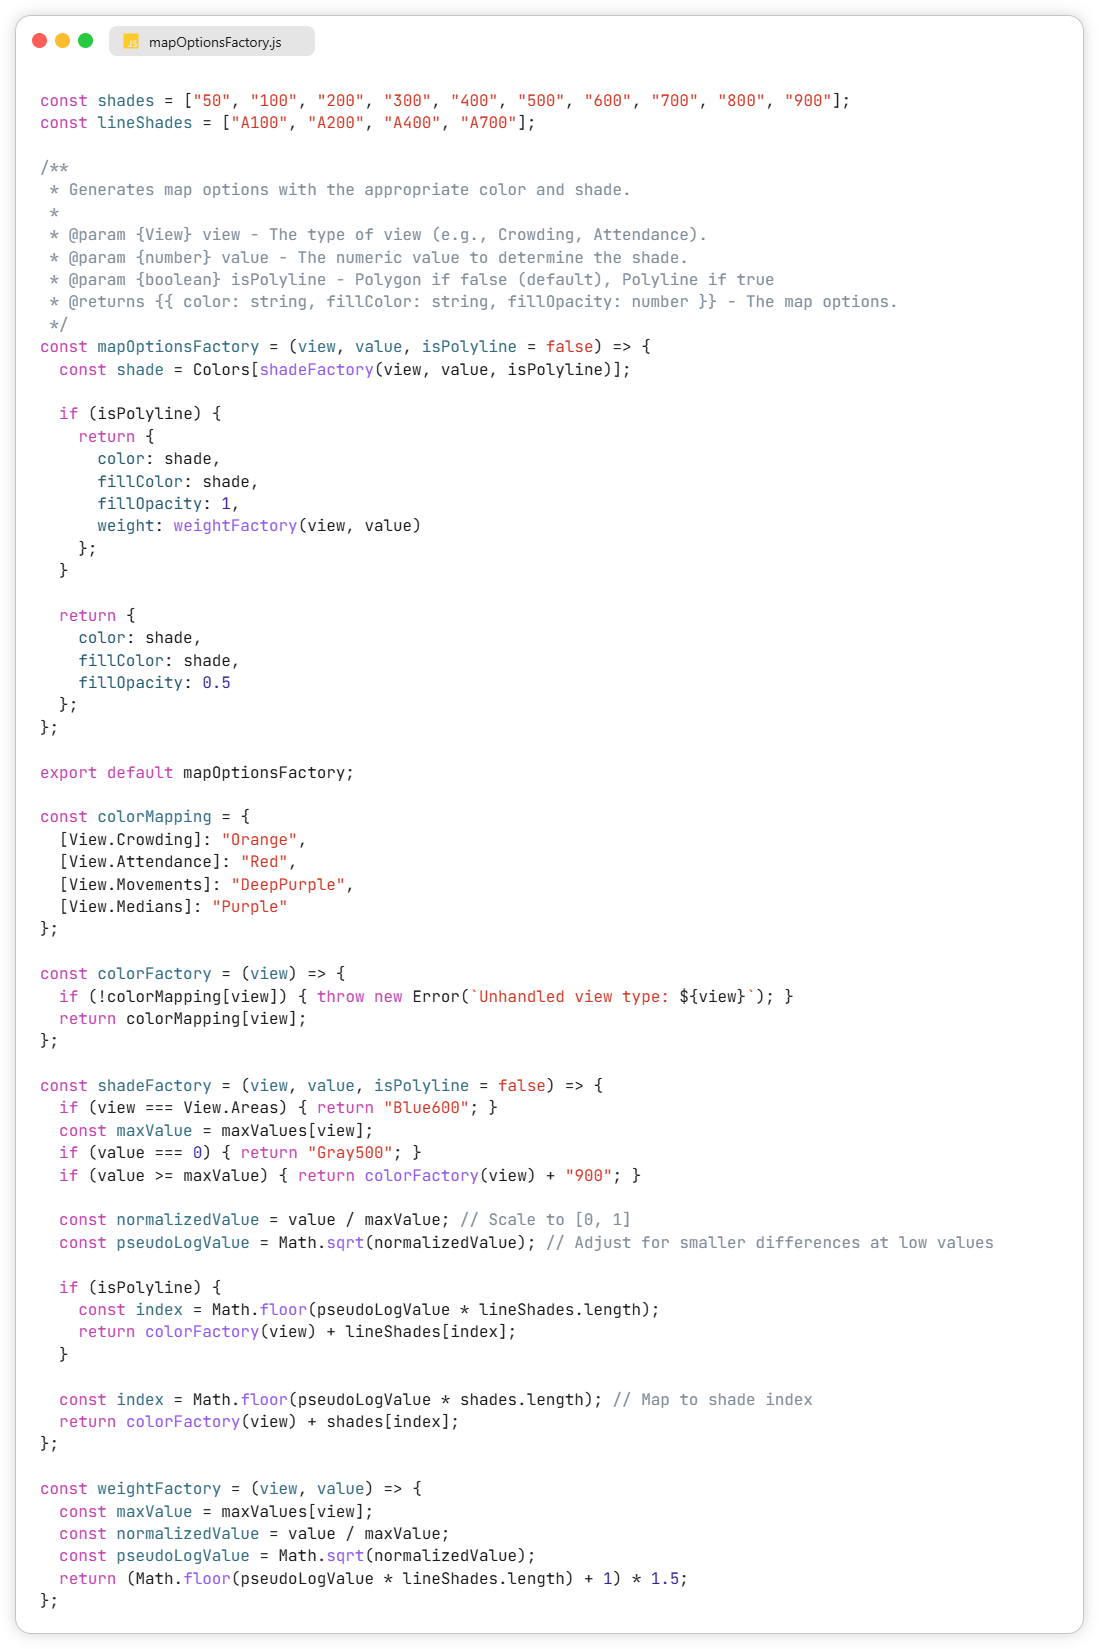
\includegraphics[width=\textwidth]{map_options_factory}
    \caption[Calcolo delle opzioni su colore e spessore]{Calcolo delle opzioni relative a colore e spessore di linee e polilinee.}
    \label{fig:map_options_factory}
\end{figure}

Per vedere un esempio di questo \textit{color coding}, in Figura~\ref{fig:mobile} possiamo vedere le quattro schermate di visualizzazione dati relative alla versione mobile, notando come il design sia sostanzialmente simile a quello già visto per quella desktop.
Vale la pena notare come l'applicazione sia stata realizzata seguendo il pattern mobile-first, quindi è per principio nata per essere mobile-friendly. Inoltre, è in grado di seguire il tema chiaro e scuro del sistema in cui si trova.

\begin{figure}[H]
    \centering
    \includegraphics[width=\textwidth]{mobile_screenshots}
    \caption[Screenshots su mobile]{Screenshots dell'applicazione su dispositivo mobile, relativi alle schermate di affollamento, affluenza, spostamenti e mediani, con il menù per cambiare la tipologia di mappa.}
    \label{fig:mobile}
\end{figure}

\section{Analisi sull'usabilità}
% 2-3 task da fare valutare agli utenti se è più facile usare il mio sistema rispetto al sito degli open data + questionario SUS
% TASK:
% - visualizzazione delle zone coperte da segnale
% - visualizzazione spostamenti degli utenti tra le varie zone
% - visualizzazione di affollamento/affluenza di una specifica zona

% OPINIONI UTENTI: in forma anonima, basta una descrizione generale sui dati aggregati
% Dati in forma aggregata, specificando il range di valori per le informazioni anagrafiche e.g. età, per il SUS invece valore medio, min e max con dettaglio per risposta.

Una volta realizzata l'applicazione web, abbiamo reclutato un gruppo di utenti affinché svolgessero un test relativo all'usabilità, confrontando il sito degli Open Data con quello da noi realizzato, ovvero BolognaWiFiMap.

Innanzitutto, dobbiamo fare qualche considerazione sul campione di utenti preso in esame, avente dimensione \( n = 9 \), con \( n \) numero di utenti. Questo campione è indubbiamente piccolo, ma sufficiente a trarre le conclusioni necessarie alla valutazione della qualità del sistema realizzato.

Riguardo all'età degli utenti, questa varia in un range tra 23 e 30 anni (media 24.7, mediana 24.0). Stiamo quindi considerando un campione abbastanza uniforme di persone giovani e aventi familiarità con il mondo digitale. L'ultima considerazione è importante perché ci permette di imputare eventuali problemi alla scarsa usabilità del sito stesso e non a una bassa capacità di interazione digitale, e viceversa rende possibile capire se un sito sia ben utilizzabile.

\section{Feedback utente su task assegnati}
Per effettuare questo test in maniera standardizzata, abbiamo definito qualche task da sottoporre agli utenti. Tali compiti sono mirati a valutare la facilità di utilizzo dell'applicazione e riguardano i seguenti aspetti:
\begin{itemize}
    \item Visualizzazione delle zone coperte da segnale.
    \item Visualizzazione degli spostamenti degli utenti tra le varie zone.
    \item Visualizzazione dell'affollamento di una specifica zona.
    \item Visualizzazione dell'affluenza di una specifica zona.
\end{itemize}

Gli utenti dovevano valutare se fosse più facile svolgere questi compiti sul sito degli Open Data o se, al contrario, risultasse più comoda l'applicazione BolognaWiFiMap realizzata da noi. Dopodiché avrebbero lasciato un feedback che sarebbe stato raccolto in maniera anonima.

Per evitare di influenzare l'opinione degli utenti, abbiamo lasciato che svolgessero il test in totale autonomia, spiegando loro in maniera chiara quali fossero gli obiettivi sui quali focalizzarsi. Al fine di fornire agli stessi una comprensione di base sugli argomenti trattati da entrambi i siti, abbiamo spiegato concisamente agli utenti i concetti di BolognaWiFi, affollamento, affluenza e spostamenti, in modo da evitare un bias sui dati dovuto a una conoscenza inesistente dell'ambiente di test.

Le nostre aspettative iniziali ritenevano il sito degli Open Data più difficile da utilizzare rispetto al nostro sistema, e abbiamo in seguito avuto conferma dalle opinioni degli utenti che tali supposizioni erano assolutamente fondate, trovando un certo livello di consistenza all'interno dei feedback forniti. Andiamo quindi ad illustrare le opinioni degli utenti relative ai due sistemi.

\subsubsection{Open Data}
% Eu: assolutamente poco pratico, però ti dice letteralmente quello che è. Non ci si potrebbe mai fare un qualcosa di comodo e vendibile a delle persone, o comunque pratico.
% Mancu: "mi sento meno gay", fa schifo in confronto al mio
% Jyulo: "esperienza assolutamente anonima" perché cercava un modo carino per dire "non ho assolutamente capito un cazzo di quello che c'è in sto sito". Immaginava cosa fosse perché glielo avevo anticipato, ma altrimenti non ne aveva assolutamente idea perché "non si capisce un cazzo". Non sa se in quel sito lì uno ci va apposta perché ci vuole andare o se ci capita per caso reindirizzato da qualche parte, in quel caso è comunque un sito assolutamente inutile e non ha senso.
Le opinioni riguardanti il sito degli Open Data sono state prevalentemente negative. 7 utenti su 9 lamentavano il fatto che l'esperienza risultasse scarsissima, confusionaria e di difficile comprensione, con un utente che l'ha definita come assolutamente anonima. Tuttavia, 2 di questi 7 utenti hanno comunque sottolineato che, benché la scarsa praticità di utilizzo, questo sito rimanga comunque utile come banca dati. Gli altri due utenti hanno invece ritenuto la loro esperienza buona o addirittura ottima.

\subsubsection{BolognaWiFiMap}
% Eu: non è difficile ma è poco intuitivo: sarebbe da rendere solo un pochino più intuitivo.
% Mancu: la mappa è un po' strana ma va beh. Molto più facile da utilizzare
% Jyulo: gran bel sito
Riguardo al nostro sito BolognaWiFiMap, invece, le opinioni si sono radicalmente capovolte. Tutti gli utenti hanno evidenziato che l'esperienza risultasse buona o ottima, con un utente che è arrivato addirittura a definirla eccellente. Inoltre, sono rimasti tutti concordi sul fatto che questo sito sia molto più facile da utilizzare rispetto a quello degli Open Data. A vari livelli, la visualizzazione dei dati è stata ritenuta rapida e intuitiva, molto efficace a livello visivo. Solo un utente ha consigliato che potrebbe essere una buona idea rendere il sito ancora più intuitivo, offrendo spiegazioni ulteriori riguardo ai vari tipi di visualizzazioni di dati, seppur rimanendo dell'idea che già ora il sito sia facilmente utilizzabile. Quest'ultimo feedback fornisce uno spunto per un possibile sviluppo futuro dell'applicazione, volto a garantirne un'ancora maggiore accessibilità.

\section{Questionario SUS}
Ottenere un feedback dagli utenti è un ottimo passo in avanti per definire possibili punti di forza e debolezze di un'applicazione, ma queste opinioni hanno una natura prettamente soggettiva. Serve quindi un modo per valutare l'usabilità di un sistema in maniera standardizzata e il più obiettiva possibile, ed è qui che entra in gioco il questionario SUS.

Il questionario SUS (\textit{System Usability Scale}) è un insieme di 10 domande di carattere generale che possono essere utilizzate per valutare l'usabilità di un qualsiasi sistema su una scala da 0 (usabilità percepita molto scarsa) a 100 (usabilità percepita eccellente) \cite{SUS}.

Questo generalismo rappresenta il suo punto di forza, in quanto è in grado di adattarsi a qualunque tipo di applicazione, ma costituisce anche la sua più grande debolezza, dato che non permette di capire su quali aree lavorare per poter migliorare l'usabilità \cite{SUS}.

All'interno delle 10 domande, quelle dispari hanno una formulazione positiva e servono a calcolare la facilità d'uso, mentre quelle pari sono formulate in modo negativo appositamente per calcolare le possibili difficoltà legate all'utilizzo, contrastando con la domanda appena posta in precedenza.

Il punteggio finale del questionario SUS viene calcolato utilizzando la formula seguente \eqref{eq:sus_original} \cite{SUS_DesignersItalia}:

\begin{equation}
    SUS = \left( \sum_{i=1,3,5,7,9} (X_i - 1) + \sum_{i=2,4,6,8,10} (5 - X_i) \right) \times 2.5
    \label{eq:sus_original}
\end{equation}

Dove \( X_i \) sono le domande \( X_1, ..., X_{10} \). Quest'ultima formula può essere semplificata nella seguente \eqref{eq:sus_simplified} \cite{SUS_Wikipedia}:

\begin{equation}
    SUS = 2.5 \times \left( 20 + \sum_{i=1,3,5,7,9} X_i - \sum_{i=2,4,6,8,10} X_i \right)
    \label{eq:sus_simplified}
\end{equation}

La quale, a sua volta, può essere riscritta in forma abbreviata \eqref{eq:sus_shortened} per ottenere una maggiore chiarezza ed efficacia di comprensione \cite{SUS_Wikipedia}:

\begin{equation}
    SUS = 2.5 \times \left( 20 + \sum (\text{SUS}_{\text{odd}}) - \sum (\text{SUS}_{\text{even}}) \right)
    \label{eq:sus_shortened}
\end{equation}

Diventa ora chiaro dalla \eqref{eq:sus_shortened} come le domande dispari, positive, contribuiscano ad aumentare il punteggio finale del SUS, mentre quelle pari, negative, lo diminuiscano. Di conseguenza, è auspicabile che gli utenti rispondano con un voto alto alle domande dispari e con uno basso per quelle pari, al fine di ottenere un punteggio elevato.

Il questionario SUS che abbiamo sottoposto agli utenti è quello fornito da Designers Italia \cite{SUS_DesignersItalia}, ma la struttura del questionario è standardizzata in tutte le lingue. Di seguito elenchiamo la lista delle domande in Tabella~\ref{tab:sus_questions}.

\begin{center}
    \begin{table}[H]
        \centering
        \begin{tabularx}{1.02\textwidth}{|c|X|}
            \hline
            \multicolumn{2}{|c|}{\textbf{Questionario SUS}} \\
            \hline
            \textbf{Domanda} & \textbf{Descrizione}\\
            \hline
            SUS01 & Penso che mi piacerebbe utilizzare questo sito frequentemente.\\
            SUS02 & Ho trovato il sito inutilmente complesso.\\
            SUS03 & Ho trovato il sito molto semplice da usare.\\
            SUS04 & Penso che avrei bisogno del supporto di una persona già in grado di utilizzare il sito.\\
            SUS05 & Ho trovato le varie funzionalità del sito bene integrate.\\
            SUS06 & Ho trovato incoerenze tra le varie funzionalità del sito.\\
            SUS07 & Penso che la maggior parte delle persone possano imparare ad utilizzare il sito facilmente.\\
            SUS08 & Ho trovato il sito molto difficile da utilizzare.\\
            SUS09 & Mi sono sentito a mio agio nell'utilizzare il sito.\\
            SUS10 & Ho avuto bisogno di imparare molti processi prima di riuscire ad utilizzare al meglio il sito.\\
            \hline
        \end{tabularx}
        \caption[Lista di domande del questionario SUS]{Lista di domande del questionario SUS.}
        \label{tab:sus_questions}
    \end{table}
\end{center}

A ciascuna di queste domande, a prescindere se sia pari o dispari, si può rispondere con un numero intero da 1 (fortemente in disaccordo) a 5 (fortemente d'accordo). Quindi, non solo la formulazione delle domande è semplice, ma lo è altrettanto la valutazione delle relative risposte.

D'ora in poi, eviteremo di riportare nuovamente la descrizione per ogni domanda, ma ci riferiremo ad esse tramite la sigla SUS01 per la prima domanda, e così via.

\section{Risposte al questionario SUS}
Andiamo ora ad analizzare le risposte fornite dagli utenti. Riporteremo dapprima ciascuna delle due tabelle con i risultati individuali degli utenti, sia per il sito degli Open Data in Tabella~\ref{tab:sus_opendata}, sia per il nostro sito BolognaWiFiMap in Tabella~\ref{tab:sus_bolognawifimap}. Infine, mostreremo la Tabella~\ref{tab:sus_avg_values} contenente la media dei risultati per ciascuna domanda. Per motivi di spazio, in Tabella~\ref{tab:sus_opendata} e Tabella~\ref{tab:sus_bolognawifimap} abbiamo abbreviato i nomi delle domande, scrivendo ad esempio S01 al posto di SUS01.

\begin{center}
    \begin{table}[H]
        \centering
        \begin{tabularx}{\textwidth}{|c|c|c|c|c|c|c|c|c|c|X|}
            \hline
            \multicolumn{11}{|c|}{\textbf{Risposte SUS Open Data}} \\
            \hline
            \textbf{S01} & \textbf{S02} & \textbf{S03} & \textbf{S04} & \textbf{S05} & \textbf{S06} & \textbf{S07} & \textbf{S08} & \textbf{S09} & \textbf{S10} & \textbf{SUS} \\
            \hline
            1 & 4 & 2 & 4 & 3 & 4 & 2 & 4 & 1 & 4 & 22.5 \\
            4 & 4 & 2 & 3 & 3 & 4 & 5 & 4 & 1 & 3 & 42.5 \\
            3 & 3 & 3 & 4 & 5 & 2 & 4 & 2 & 3 & 3 & 60.0 \\
            2 & 2 & 3 & 3 & 3 & 2 & 4 & 2 & 3 & 1 & 62.5 \\
            1 & 5 & 1 & 4 & 1 & 4 & 2 & 2 & 2 & 1 & 27.5 \\
            3 & 2 & 4 & 2 & 4 & 1 & 5 & 2 & 5 & 1 & 82.5 \\
            1 & 2 & 3 & 5 & 2 & 4 & 1 & 4 & 2 & 4 & 25.0 \\
            4 & 2 & 3 & 4 & 5 & 2 & 3 & 3 & 5 & 2 & 67.5 \\
            1 & 4 & 2 & 3 & 1 & 3 & 1 & 4 & 1 & 3 & 22.5 \\
            \hline
        \end{tabularx}
        \caption[Risposte del questionario SUS sul sito degli Open Data]{Risposte fornite dagli utenti sul questionario SUS relativo al sito degli Open Data, in forma anonima.}
        \label{tab:sus_opendata}
    \end{table}
\end{center}

\begin{center}
    \begin{table}[h]
        \centering
        \begin{tabularx}{\textwidth}{|c|c|c|c|c|c|c|c|c|c|X|}
            \hline
            \multicolumn{11}{|c|}{\textbf{Risposte SUS BolognaWiFiMap}} \\
            \hline
            \textbf{S01} & \textbf{S02} & \textbf{S03} & \textbf{S04} & \textbf{S05} & \textbf{S06} & \textbf{S07} & \textbf{S08} & \textbf{S09} & \textbf{S10} & \textbf{SUS} \\
            \hline
            5 & 1 & 5 & 2 & 5 & 1 & 5 & 1 & 5 & 1 & 97.5 \\
            5 & 1 & 5 & 1 & 5 & 1 & 5 & 1 & 5 & 1 & 100 \\
            4 & 2 & 4 & 3 & 4 & 1 & 4 & 2 & 3 & 1 & 75.0 \\
            3 & 1 & 5 & 1 & 5 & 2 & 5 & 1 & 5 & 2 & 90.0 \\
            3 & 2 & 4 & 2 & 4 & 2 & 4 & 2 & 4 & 1 & 75.0 \\
            4 & 2 & 5 & 1 & 4 & 2 & 4 & 2 & 5 & 1 & 85.0 \\
            4 & 1 & 5 & 1 & 5 & 1 & 5 & 1 & 5 & 1 & 97.5 \\
            5 & 2 & 3 & 4 & 5 & 2 & 3 & 2 & 4 & 2 & 70.0 \\
            4 & 1 & 5 & 1 & 5 & 1 & 5 & 1 & 5 & 1 & 97.5 \\
            \hline
        \end{tabularx}
        \caption[Risposte del questionario SUS sul sito BolognaWiFiMap]{Risposte fornite dagli utenti sul questionario SUS relativo al sito BolognaWiFiMap, in forma anonima.}
        \label{tab:sus_bolognawifimap}
    \end{table}
\end{center}

\begin{center}
    \begin{table}[H]
        \centering
        \begin{tabularx}{\textwidth}{|X|X|X|}
            \hline
            \multicolumn{3}{|c|}{\textbf{Valori medi risultati questionario SUS}} \\
            \hline
            \textbf{Domanda} & \textbf{Open Data} & \textbf{BolognaWiFiMap} \\
            \hline
            SUS01 & 2.22 & 4.11 \\
            SUS02 & 3.11 & 1.44 \\
            SUS03 & 2.56 & 4.56 \\
            SUS04 & 3.56 & 1.78 \\
            SUS05 & 3.00 & 4.67 \\
            SUS06 & 2.89 & 1.44 \\
            SUS07 & 3.00 & 4.44 \\
            SUS08 & 3.00 & 1.44 \\
            SUS09 & 2.56 & 4.56 \\
            SUS10 & 2.44 & 1.22 \\
            \hline
            \textbf{Punteggio SUS} & \textbf{45.8} & \textbf{87.5} \\
            \hline
            \textbf{Media Dispari} & 2.67 & 4.47 \\
            \textbf{Media Pari} & 3.00 & 1.47 \\
            \hline
            \textbf{Mediana Dispari} & 2.56 & 4.56 \\
            \textbf{Mediana Pari} & 3.00 & 1.44 \\
            \hline
            \textbf{Dev. Std. Dispari} & 0.333 & 0.214 \\
            \textbf{Dev. Std. Pari} & 0.401 & 0.199 \\
            \hline
        \end{tabularx}
        \caption[Valori medi totali e per domanda del questionario SUS]{Valori medi per ciascuna domanda del questionario SUS. Viene inoltre calcolato per ciascun sito il punteggio medio complessivo risultante da tutti gli utenti. Quindi, distinguendo tra domande dispari e pari, si determinano media, mediana e deviazione standard per ciascuna delle due categorie positive e negative.}
        \label{tab:sus_avg_values}
    \end{table}
\end{center}

\begin{figure}[H]
    \centering
    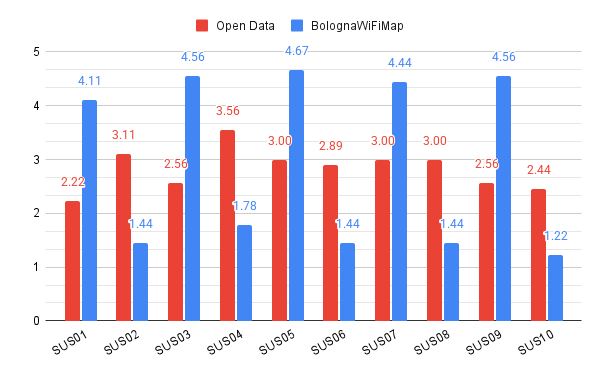
\includegraphics[width=\textwidth]{sus_avg_values_legend}
    \caption[Valori medi per ciascuna domanda del questionario SUS]{Valori medi per ciascuna domanda del questionario SUS. In rosso, quelli relativi al sito degli Open Data. In blu, quelli su BolognaWiFiMap.}
    \label{fig:sus_avg_values}
\end{figure}

\section{Valutazione dei risultati complessivi}
Possiamo già notare dalla Tabella~\ref{tab:sus_avg_values} come complessivamente BolognaWiFiMap batta gli Open Data su tutte le possibili metriche, a cominciare da un punteggio SUS quasi doppio. Sia nelle domande pari, che nelle domande dispari, la differenza tra media e mediana è molto piccola, segno di un insieme di dati piuttosto consistenti e senza particolari \textit{outliers}. Questa affermazione è ulteriormente supportata, per entrambe le tipologie di domanda, da una deviazione standard (abbastanza) piccola, che indica una bassa dispersione dei dati.

In particolare, diventa evidente come il valore medio e mediano delle domande dispari (positive) relativo a BolognaWiFiMap sia molto più elevato rispetto a quello degli Open Data. Allo stesso modo, il valore medio e mediano delle domande pari (negative) di BolognaWiFiMap risulta essere più basso di quello sugli Open Data, seppur con un margine inferiore rispetto alle domande dispari. Possiamo facilmente vedere queste differenze in maniera grafica in Figura~\ref{fig:sus_avg_values}. Relativamente ai criteri di valutazione delle domande pari e dispari, seppur con vario margine, non esiste nessun caso in cui il sito degli Open Data abbia performato meglio di BolognaWiFiMap.

Notiamo comunque come, relativamente alle categorie di domande pari e dispari, il sito degli Open Data abbia ottenuto una varianza maggiore nelle risposte rispetto a BolognaWiFiMap, indicando opinioni leggermente più contrastanti. Ciò è riscontrabile dal valore maggiore della deviazione standard, specialmente nelle domande pari. Questo ci fa pensare che ciascun utente abbia criteri di usabilità differenti, che diventano particolarmente evidenti quando si tratta di giudicare un sito non propriamente facile da utilizzare. D'altro canto, gli utenti sono stati più concordi nel giudizio di BolognaWiFiMap, cosa visibile sempre dalla deviazione standard.

\section{Risultati per ciascun utente}
Se complessivamente possiamo già decretare BolognaWiFiMap come sito avente l'usabilità migliore, non possiamo ancora trarre conclusioni relative alle preferenze di ciascun singolo utente. Andiamo quindi a vedere i risultati che ogni persona ha ottenuto nel questionario SUS relativo a entrambi i siti, in Tabella~\ref{tab:sus_scores}.

\begin{center}
    \begin{table}[H]
        \centering
        \begin{tabularx}{\textwidth}{|
            >{\hsize=0.5\hsize}X|
            >{\hsize=0.5\hsize}X|
            X|
            X|}
            \hline
            \multicolumn{4}{|c|}{\textbf{Confronto risultati SUS}} \\
            \hline
            \textbf{Utente} & \textbf{Età} & \textbf{Open Data} & \textbf{BolognaWiFiMap} \\
            \hline
            U01 & 24 & 22.5 & 97.5 \\
            U02 & 23 & 42.5 & 100 \\
            U03 & 23 & 60.0 & 75.0 \\
            U04 & 24 & 62.5 & 90.0 \\
            U05 & 23 & 27.5 & 75.0 \\
            U06 & 26 & 82.5 & 85.0 \\
            U07 & 24 & 25.0 & 97.5 \\
            U08 & 25 & 67.5 & 70.0 \\
            U09 & 30 & 22.5 & 97.5 \\
            \hline
            \multicolumn{2}{|X|}{\textbf{Punteggio medio}} & \textbf{45.8} & \textbf{87.5} \\
            \hline
            \multicolumn{2}{|X|}{\textbf{Min.}} & 22.5 & 70.0 \\
            \hline
            \multicolumn{2}{|X|}{\textbf{Max.}} & 82.5 & 100 \\
            \hline
            \multicolumn{2}{|X|}{\textbf{Mediana}} & 42.5 & 90.0 \\
            \hline
            \multicolumn{2}{|X|}{\textbf{Dev. Std.}} & 22.8 & 11.7 \\
            \hline
            \multicolumn{2}{|X|}{\textbf{\( \boldsymbol{\rho} \) di Spearman}} & 0.0693 & 0.00 \\
            \hline
        \end{tabularx}
        \caption[Punteggi ottenuti dagli utenti nel questionario SUS]{Punteggi ottenuti dagli utenti nel questionario SUS. Viene quindi calcolato il punteggio medio complessivo, insieme a mediana, deviazione standard, e coefficiente di correlazione \( \rho \) di Spearman.}
        \label{tab:sus_scores}
    \end{table}
\end{center}

Anche qui notiamo chiaramente come nessun utente abbia mostrato una netta preferenza per il sito degli Open Data, seppur in due casi BolognaWiFiMap abbia ottenuto solo un leggerissimo vantaggio. Questo diventa particolarmente facile da vedere in maniera grafica dalla Figura~\ref{fig:sus_scores}.

Come prima, la media dei punteggi complessivi non si discosta molto dalla mediana, in linea con quanto è avvenuto per ciascuna risposta in Tabella~\ref{tab:sus_avg_values}, quindi l'insieme di dati è piuttosto consistente e non presenta particolari \textit{outliers}.

La deviazione standard, anche in questo caso, è maggiore per gli Open Data rispetto che a BolognaWiFiMap, segno di una più grande varianza tra le risposte e quindi di opinioni leggermente più contrastanti.

Per valutare la relazione tra l'età degli utenti e la percezione dell'usabilità, abbiamo utilizzato il coefficiente di correlazione \( \rho \) di Spearman , in quanto a differenza di quello di Pearson \( r \), non assume una distribuzione normale, è meno sensibile agli \textit{outliers} e misura la correlazione monotona tra due variabili. Di conseguenza è più adatto per piccoli campioni di dati e per relazioni non necessariamente lineari, come nel nostro caso.

Il coefficiente di correlazione di Spearman ( \( \rho \) ) è calcolato utilizzando la seguente formula:
\begin{equation}
    \rho = 1 - \frac{6 \sum d_i^2}{n(n^2 - 1)}
    \label{eq:spearman_correlation_coefficient}
\end{equation}

Dove \( n \) è il numero di punti (dati) a disposizione e \( d_i^2 \) è il quadrato della differenza tra i ranghi di \( x_i \) e \( y_i \), ovvero:

\begin{equation}
    d_i = R(x_i) - R(y_i)
    \label{eq:rank_difference}
\end{equation}

\begin{equation}
    d_i^2 = (R(x_i) - R(y_i))^2
    \label{eq:squared_rank_difference}
\end{equation}

Dove \( R(x_i) \) e \( R(y_i) \) sono definiti come:

\begin{equation}
    R(x_i) = \text{Rango di } x_i \quad \text{(posizione di } x_i \text{ nella lista dei valori } x_1, ..., x_n \text{)}
    \label{eq:rank_x}
\end{equation}

\begin{equation}
    R(y_i) = \text{Rango di } y_i \quad \text{(posizione di } y_i \text{ nella lista dei valori } y_1, ..., y_n \text{)}
    \label{eq:rank_y}
\end{equation}

Il coefficiente di correlazione \( \rho \) di Spearman varia tra -1 e +1:
\begin{itemize}
    \item \( \rho = +1 \rightarrow \) Correlazione perfetta positiva.
    \item \( \rho = -1 \rightarrow \) Correlazione perfetta negativa.
    \item \( \rho = 0 \rightarrow \) Nessuna correlazione monotona.
\end{itemize}

Se \( \rho > 0 \) esiste una correlazione positiva, mentre se \( \rho < 0 \) esiste una correlazione negativa. Riguardo al valore in sé della correlazione, \( |\rho| < 0.3 \) indica una correlazione debole, \( |\rho| \in [0.3, 0.7] \) denota una correlazione moderata, mentre \( |\rho| > 0.7 \) mostra una correlazione forte.

I risultati ottenuti indicano che non esiste alcuna correlazione significativa tra l'età degli utenti e i punteggi SUS, suggerendo quindi che la percezione dell'usabilità dell'applicazione sia indipendente dall'età.

\begin{figure}[H]
    \centering
    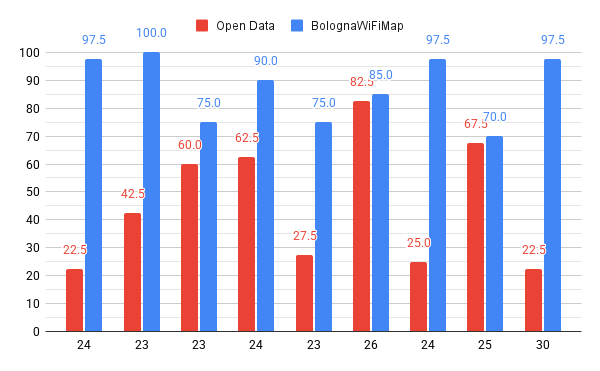
\includegraphics[width=\textwidth]{sus_scores_legend}
    \caption[Punteggi ottenuti nel questionario SUS]{Punteggi ottenuti dagli utenti nel questionario SUS, evidenziando l'età di ciascun utente in ascissa. In rosso, quelli relativi al sito degli Open Data. In blu, quelli su BolognaWiFiMap.}
    \label{fig:sus_scores}
\end{figure}

Il punteggio SUS può essere convertito in un voto utilizzando una tabella di conversione che lo trasforma utilizzando il sistema di valutazione americano \cite{SUS}. Tali criteri sono visibili in Tabella~\ref{tab:sus_grading_system}.

La valutazione dei punteggi SUS di ciascun utente è visibile in Tabella~\ref{tab:sus_grades}. In base alla scala di valutazione del SUS, il sito degli Open Data otterrebbe mediamente come voto F, mentre BolognaWiFiMap si guadagnerebbe in media un solido A+. La mediana assumerebbe gli stessi valori.

Riguardo agli estremi, il voto minimo di Open Data sarebbe sempre una F, mentre quello massimo sarebbe una A. BolognaWiFiMap, invece, ha come voto minimo una C, ma quello massimo rimane sempre una A+.

Possiamo notare come solo due utenti abbiano fornito una valutazione dei due siti pressoché equivalente, mentre in tutti gli altri casi la differenza è ben più drastica e a favore di BolognaWiFiMap.

\begin{center}
    \begin{table}[H]
        \centering
        \begin{tabularx}{\textwidth}{|X|X|X|}
            \hline
            \textbf{Voto} & \textbf{Punteggio SUS} & \textbf{Percentile} \\
            \hline
            A+  & 84.1 -- 100   & 96 -- 100 \\
            A   & 80.8 -- 84.0  & 90 -- 95  \\
            A-  & 78.9 -- 80.7  & 85 -- 89  \\
            B+  & 77.2 -- 78.8  & 80 -- 84  \\
            B   & 74.1 -- 77.1  & 70 -- 79  \\
            B-  & 72.6 -- 74.0  & 65 -- 69  \\
            C+  & 71.1 -- 72.5  & 60 -- 64  \\
            C   & 65.0 -- 71.0  & 41 -- 59  \\
            C-  & 62.7 -- 64.9  & 35 -- 40  \\
            D   & 51.7 -- 62.6  & 15 -- 34  \\
            F   & 0 -- 51.6     & 0 -- 14   \\
            \hline
        \end{tabularx}
        \caption[Calcolo del voto a partire dal punteggio SUS]{Calcolo del voto a partire dal punteggio SUS, utilizzando il sistema di valutazione americano \cite{SUS}.}
        \label{tab:sus_grading_system}
    \end{table}
\end{center}

\begin{center}
    \begin{table}[H]
        \centering
        \begin{tabularx}{\textwidth}{|
            >{\hsize=0.5\hsize}X|
            >{\hsize=0.5\hsize}X|
            X|
            X|}
            \hline
            \multicolumn{4}{|c|}{\textbf{Valutazione SUS per utente}} \\
            \hline
            \textbf{Utente} & \textbf{Età} & \textbf{Open Data} & \textbf{BolognaWiFiMap} \\
            \hline
            U01 & 24 & F & A+ \\
            U02 & 23 & F & A+ \\
            U03 & 23 & D & B  \\
            U04 & 24 & D & A+ \\
            U05 & 23 & F & B  \\
            U06 & 26 & A & A+ \\
            U07 & 24 & F & A+ \\
            U08 & 25 & C & C  \\
            U09 & 30 & F & A+ \\
            \hline
            \multicolumn{2}{|X|}{\textbf{Punteggio medio}} & \textbf{F} & \textbf{A+} \\
            \hline
            \multicolumn{2}{|X|}{\textbf{Min.}} & F & C \\
            \hline
            \multicolumn{2}{|X|}{\textbf{Max.}} & A & A+ \\
            \hline
            \multicolumn{2}{|X|}{\textbf{Mediana}} & F & A+ \\
            \hline
        \end{tabularx}
        \caption[Valutazione del SUS per ciascun utente]{Valutazione del voto relativo al punteggio SUS di ciascun utente, utilizzando i criteri in Tabella~\ref{tab:sus_grading_system}}
        \label{tab:sus_grades}
    \end{table}
\end{center}

\clearpage{\pagestyle{empty}\cleardoublepage}

\chapter*{Conclusioni}

\rhead[\fancyplain{}{\bfseries
CONCLUSIONI}]{\fancyplain{}{\bfseries\thepage}}
\lhead[\fancyplain{}{\bfseries\thepage}]{\fancyplain{}{\bfseries
CONCLUSIONI}}

\addcontentsline{toc}{chapter}{Conclusioni}

Questa tesi ha esplorato le potenzialità degli Open Data nella gestione e ottimizzazione dei servizi urbani, con particolare attenzione alla rete BolognaWiFi. L'obiettivo del progetto era sviluppare un'applicazione web interattiva per la visualizzazione e l'analisi dei dati relativi all'uso della rete WiFi pubblica del Comune di Bologna. Attraverso lo sviluppo di un'interfaccia intuitiva e dinamica, è stato possibile rendere accessibili e interpretabili le informazioni raccolte, fornendo uno strumento utile per amministratori pubblici, ricercatori e cittadini.

L'analisi dei dati raccolti ha permesso di individuare tendenze significative nell'utilizzo della rete, evidenziando pattern di affluenza e spostamento. La rappresentazione grafica di queste informazioni si è rivelata essenziale per facilitare la comprensione e l'elaborazione di strategie di miglioramento della connettività urbana. L'adozione di tecnologie moderne come Vue.js e Leaflet ha garantito un'interfaccia interattiva e altamente performante, migliorando l'esperienza utente e rendendo la navigazione più fluida ed efficace.

Uno degli aspetti più rilevanti emersi durante il progetto è stata la necessità di un'integrazione sempre più spinta tra i dati della rete WiFi e altri dataset relativi alla mobilità urbana, al turismo e alla gestione dei servizi pubblici. Questa sinergia potrebbe rappresentare un passo avanti nella costruzione di strumenti predittivi basati sull'analisi dei dati in tempo reale, favorendo una pianificazione urbana più intelligente e reattiva alle esigenze dei cittadini.

\section*{Sviluppi futuri}

Pur avendo raggiunto gli obiettivi prefissati, il progetto può essere ulteriormente ampliato e migliorato sotto diversi aspetti. Tra le possibili evoluzioni future si possono individuare le seguenti direzioni:

\begin{itemize}
    \item \textbf{Integrazione con ulteriori dataset}: Espandere l'applicazione integrando dati relativi alla mobilità cittadina, all'occupazione degli spazi pubblici e ai flussi turistici, per fornire una visione più completa e dettagliata del comportamento urbano.
    \item \textbf{Miglioramento delle prestazioni}: Ottimizzare il caricamento dei dati e la reattività dell'interfaccia per garantire una maggiore scalabilità dell'applicazione anche in presenza di volumi elevati di informazioni.
    \item \textbf{Implementazione di modelli predittivi}: Sviluppare algoritmi di machine learning per analizzare i dati storici e prevedere i futuri trend di utilizzo della rete WiFi, supportando così le decisioni strategiche delle amministrazioni pubbliche.
    \item \textbf{Espansione del progetto ad altre città}: Applicare il modello sviluppato in questa tesi ad altre città, adattandolo alle specifiche esigenze territoriali e alle diverse infrastrutture di rete disponibili.
    \item \textbf{Miglioramento dell'interfaccia utente}: Raffinare l'esperienza utente attraverso test di usabilità e raccolta di feedback per rendere l'applicazione ancora più intuitiva e accessibile.
\end{itemize}

L'adozione di queste migliorie potrebbe trasformare l'applicazione sviluppata in un riferimento per la gestione e l'analisi dei dati urbani, promuovendo un uso più consapevole ed efficace delle risorse digitali a disposizione delle città.

\section*{Conclusione generale}

In conclusione, il lavoro svolto ha dimostrato come l'uso intelligente degli Open Data possa migliorare significativamente la gestione e la pianificazione urbana. L'integrazione di strumenti di visualizzazione avanzati consente di sfruttare al meglio il potenziale dei dati pubblici, offrendo benefici concreti per la collettività. Grazie a questo progetto, è stato possibile non solo facilitare l'accesso alle informazioni sulla rete BolognaWiFi, ma anche proporre un modello replicabile per altre realtà urbane interessate alla valorizzazione dei propri dati.

L'auspicio è che questa ricerca possa costituire un punto di partenza per ulteriori sviluppi nell'ambito della gestione delle infrastrutture digitali cittadine, contribuendo a rendere le città più connesse, intelligenti e a misura di cittadino.


%\input{./Appendice/appendice.tex}

\rhead[\fancyplain{}{\bfseries \leftmark}]{\fancyplain{}{\bfseries
\thepage}}

\clearpage{\pagestyle{empty}\cleardoublepage}
\chapter*{Ringraziamenti}
\thispagestyle{empty}

\addcontentsline{toc}{chapter}{Ringraziamenti}

% Qui possiamo ringraziare il mondo intero!!!!!!!!!!\\
% Ovviamente solo se uno vuole, non \`e obbligatorio.

Voglio ringraziare tutti coloro che mi hanno \sout{sopportato} supportato durante tutti questi anni.

\phantomsection % Enables an unnamed section to be referenced correctly in the table of contents
\addcontentsline{toc}{chapter}{Bibliografia}

\renewcommand{\bibname}{Bibliografia} % Change title of bibliography for article class, use {\bibname} for report or book class, use {\refname} for article class
\newpage
\bibliography{back/biblio}{}

%\bibliographystyle{unsrt}
\bibliographystyle{unsrtnat}

% \bibliographystyle{plainurl} % Use unsrturl to display an unsorted list



\nocite{*}

%\cleardoublepage

%\listoffigures
%\listoftables


\end{document}
